As indicated in Figure~\ref{fig:sigRegionBG}, different Standard Model processes contribute to the event sample in the signal region. To distinguish a potential signal from these backgrounds, a precise estimation of the background contributions is mandatory. While the simulation of these processes and the response of the CMS detector gives a good description of the data for the majority of the phase space, a large number of uncertainty sources are introduced in the modelling of the physical process and the detector. Therefore a higher precision can be achieved by deriving the background estimates directly from the recorded data. The background processes are categorized as either being flavour-symmetric or as containing the production of a Z boson. A dedicated method is applied for each of the two categories. The different background processes are:

\section{Flavour-symmetric backgrounds}
Processes that are symmetric in the production of same-flavour and opposite-flavour lepton pairs allow for the estimation of their contribution to the SF event sample from the OF one. The most dominant of these processes is the dileptonic decay of top-pair production, where the leptons are produced uncorrelatedly in the decay of the W bosons. Other examples are the decays of two $\tau$ leptons, which are in turn produced in the decay of a Z boson or the dileptonic decay of W pairs. Another contribution to this class of backgrounds are misidentified leptons, as will be demonstrated later. 

No significant deviation from flavour-symmetry has been observed in the decays of the W boson, with a measured ratio of the branching fractions into $e+\nu$ and $\mu + \nu$ of $1.007\pm0.021$. In the decays of the $\tau$ lepton the different masses of electron and muon have a noticeable effect, resulting in a slightly favoured decay into electrons. Here the ratio of branching fractions is $1.0241\pm0.0032$~\cite{PDG}. As backgrounds with $\tau$ leptons are a sub-dominant contribution to the the flavour-symmetric backgrounds, these can be considered to be fully flavour-symmetric on particle level. However, distortions of the flavour-symmetry are introduced by the different efficiencies for triggering, reconstructing, and identifying electrons and muons in CMS. The background estimation from OF events therefore has to include a correction for this deviation, which is applied as a multiplicative factor:
\begin{equation}
N_{SF}^{pred} = \Rsfof \cdot N_{OF}.
\end{equation}
Similarly, the factors \Reeof and \Rmmof are used to derive separate background estimates for the \EE and \MM channel separately. Two independent methods are utilized to measure \Rsfof on data. In the first approach is is directly measured as the ratio of SF to OF events in the control region for flavour-symmetric backgrounds. The second approach studies the lepton efficiencies and derives \Rsfof factorized into the effects of trigger efficiencies and reconstruction and identification efficiencies.  

\subsection{Direct measurement of \Rsfof}
The ratio of SF to OF events as a function of \mll in simulation is shown in Figure~\ref{fig:controlRatioMC}, separately for the central and forward lepton selection. The ratio is very close to on and independent of \mll, except at the \Z peak. It can be concluded that an universal factor can be applied for flavour-symmetric backgrounds over the full mass range. To exclude the \Z peak from the calculation only events in the mass regions $\unit{20}{\giga\electronvolt}< \mll < \unit{70}{\giga\electronvolt}$ and $\mll > \unit{120}{\giga\electronvolt}$ are considered.   	
\begin{figure}
\begin{center}
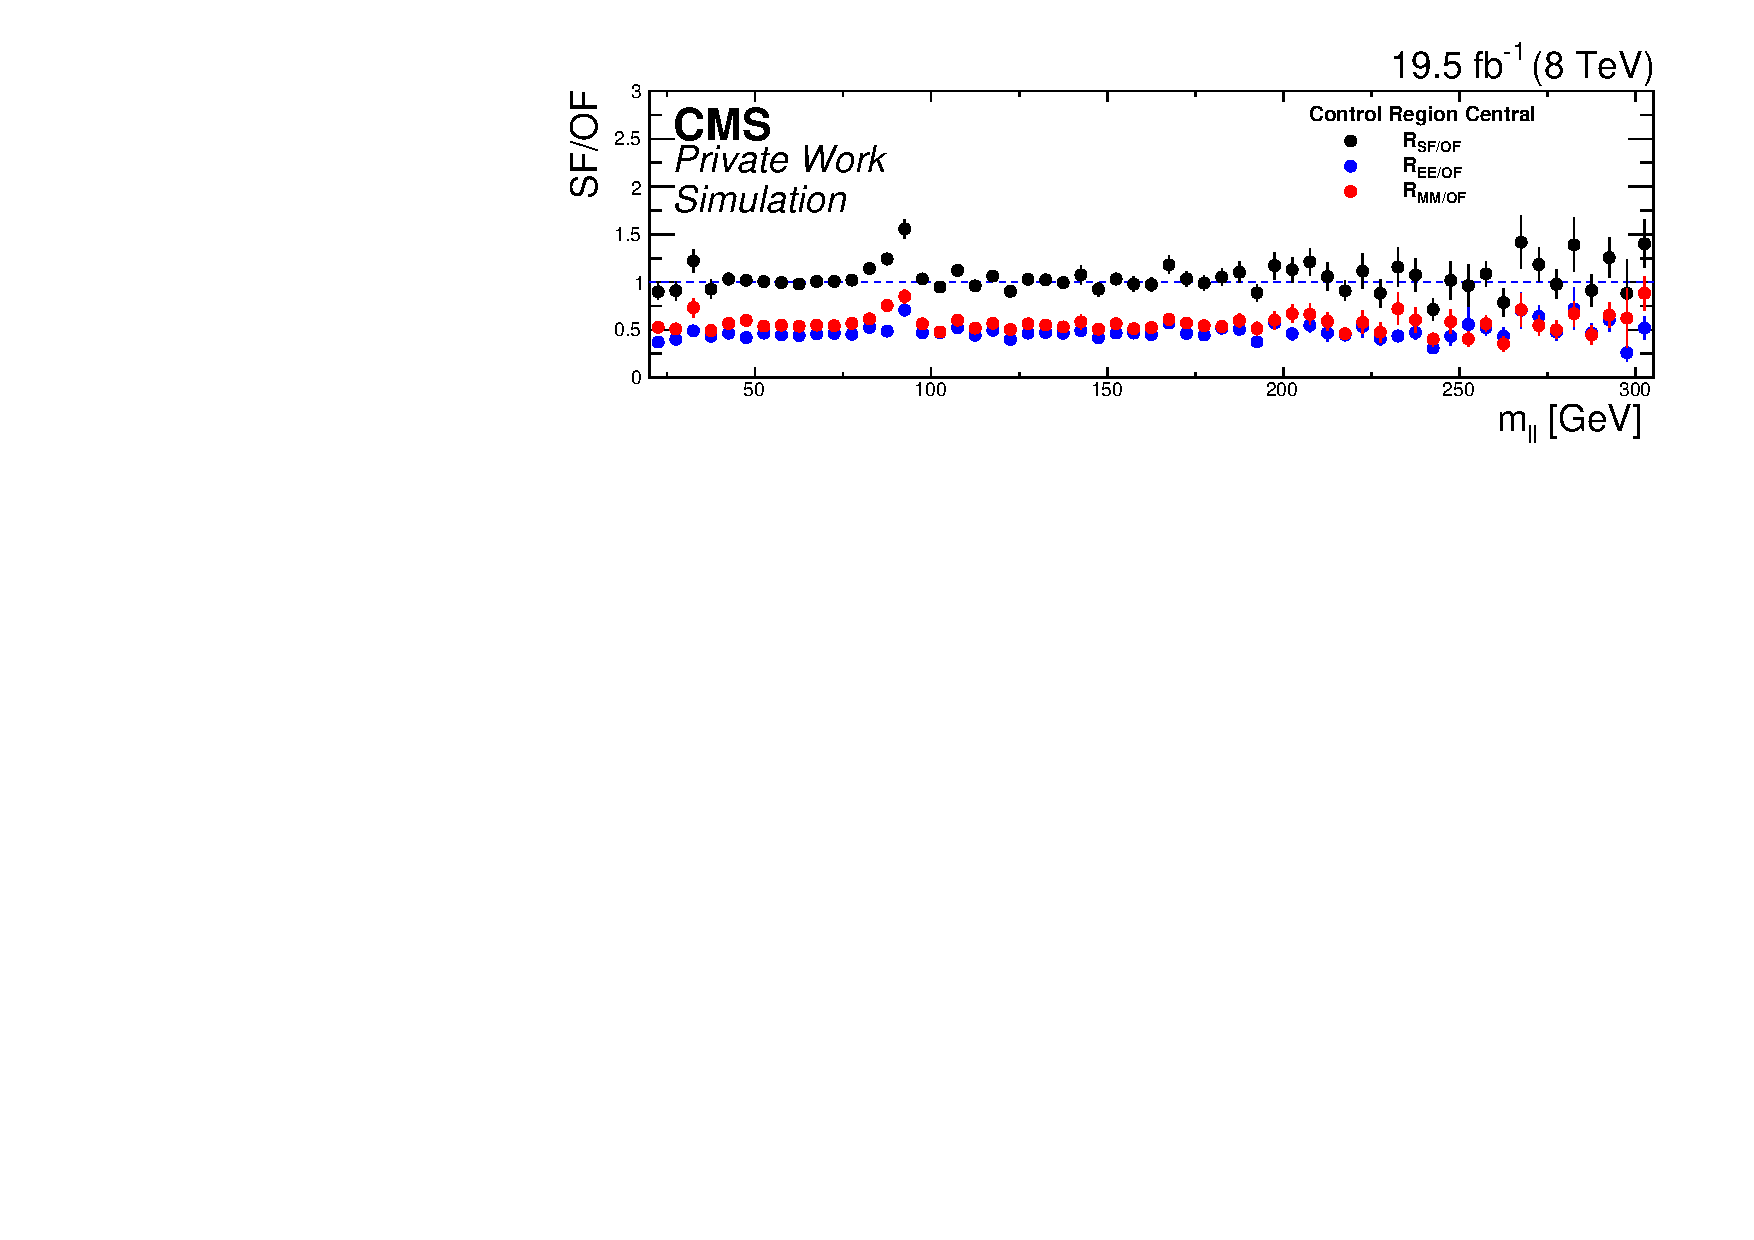
\includegraphics[scale=0.4]{plots/BG/control/rSFOF_ControlCentral_Full2012_Mll_None_MC.pdf}\\
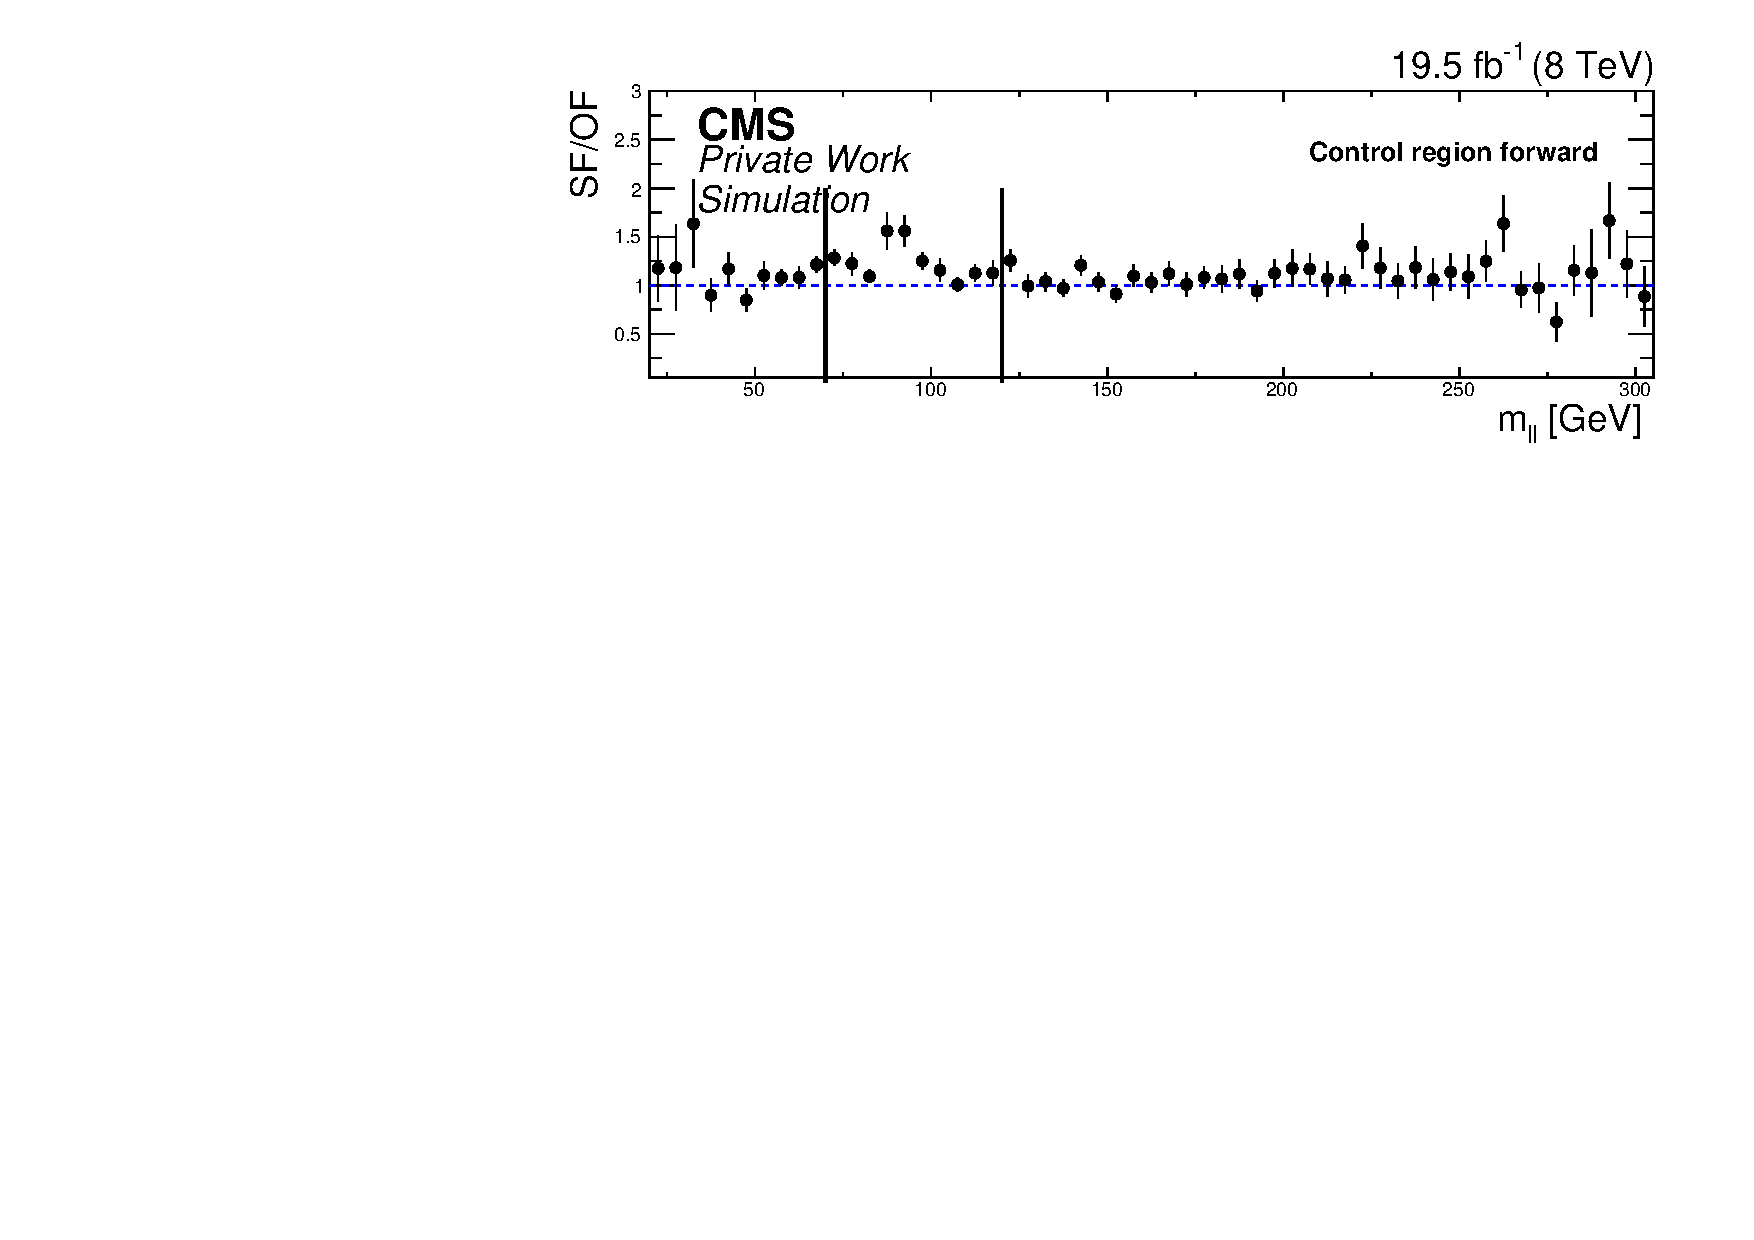
\includegraphics[scale=0.4]{plots/BG/control/rSFOF_ControlForward_Full2012_Mll_None_MC.pdf}
\caption{Ratio of SF to OF events as a function of \mll in the $t\bar{t}$ control region in simulation. Shown are the results for the central (top) and forward (bottom) lepton selection.}
\label{fig:controlRatioMC}
\end{center}
\end{figure}
The observed ratio on data as a functions of \mll is shown in Figure~\ref{fig:controlRatio}. Also here no significant dependence on \mll is observed both in the central and forward signal lepton selection.
\begin{figure}
\begin{center}
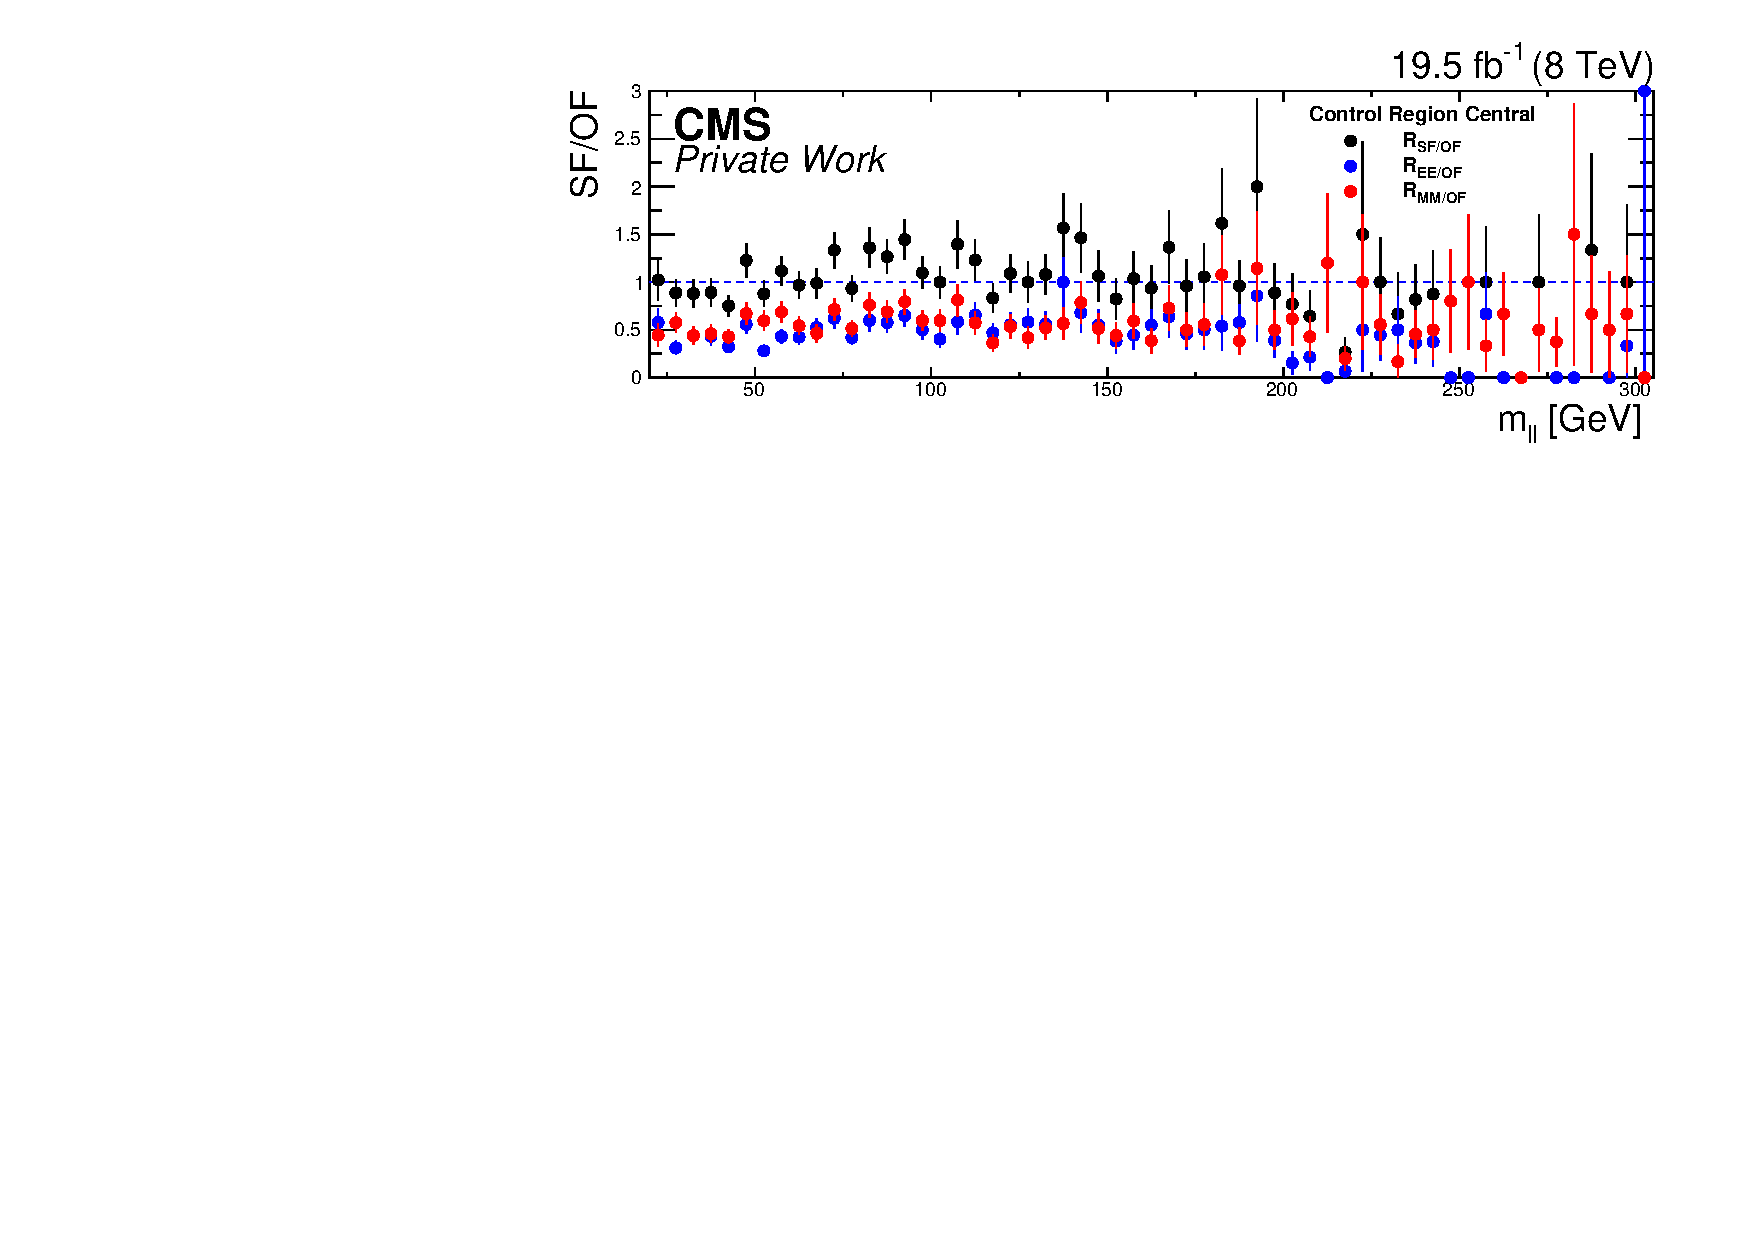
\includegraphics[scale=0.4]{plots/BG/control/rSFOF_ControlCentral_Full2012_Mll_None.pdf}\\
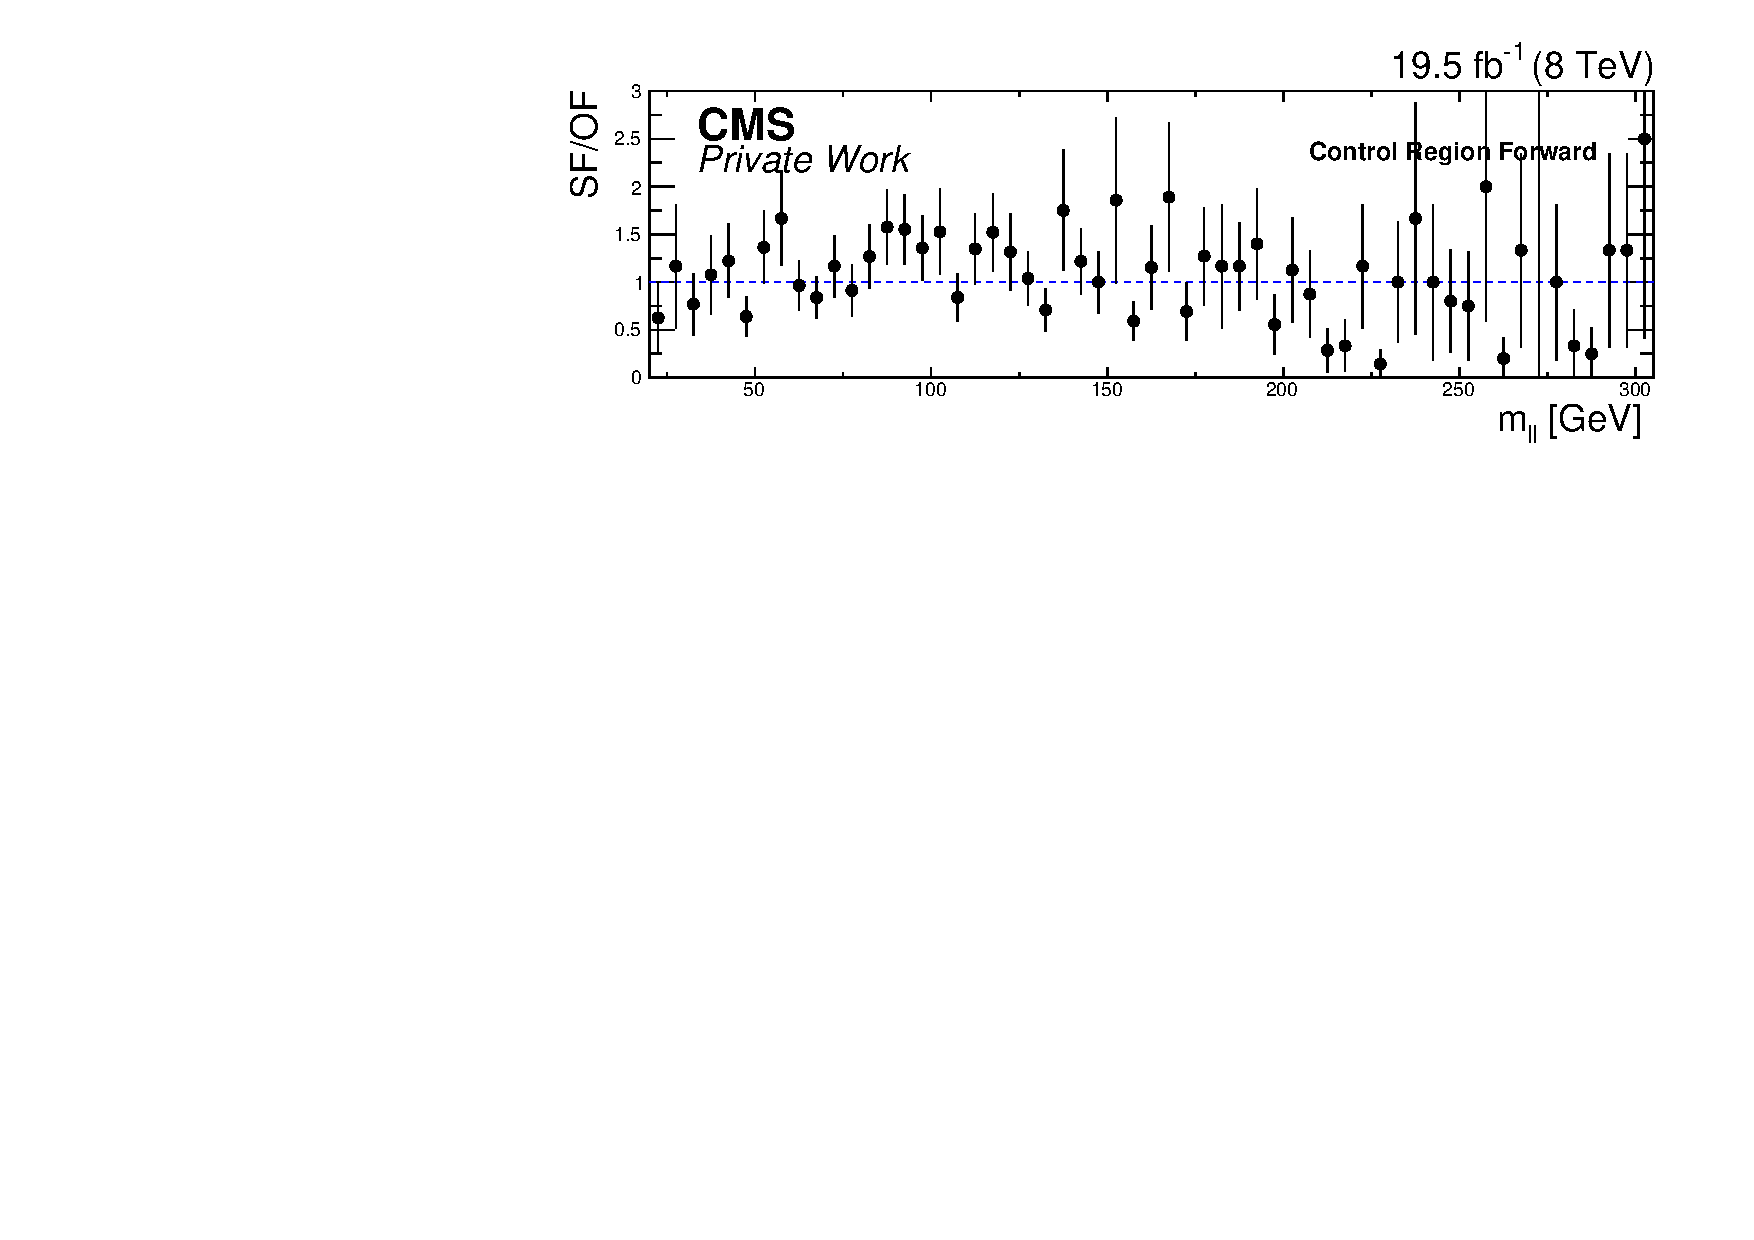
\includegraphics[scale=0.4]{plots/BG/control/rSFOF_ControlForward_Full2012_Mll_None.pdf}
\caption{Ratio of SF to OF events as a function of \mll in the $t\bar{t}$ control region in data. Shown are the results for the central (top) and forward (bottom) lepton selection.}
\label{fig:controlRatio}
\end{center}
\end{figure}
The numerical results are summarized in Table~\ref{tab:rSFOF} for \Rsfof as well as \Reeof and \Rmmof. Good agreement between the values measured in data and simulation is observed. The extrapolation of the measured value of \Rsfof into the signal region is studied in simulation. No deviation of the values measured in the signal region from those obtained in the control region is observed within the statistical uncertainties of the simulation. This uncertainty is therefore assigned as an systematic uncertainty of the method. 


\begin{table}[hbtp]
 \renewcommand{\arraystretch}{1.3}
 \setlength{\belowcaptionskip}{6pt}
 \centering
 \caption{Observed event yields in the control region and the resulting values of \Rsfof, \Reeof, and \Rmmof. The results are shown separately for the central and forward lepton selection and the same quantities derived on simulation are shown for comparison. For the simulation, the ratio between the values of \Rsfof, \Reeof, and \Rmmof measured in the signal and control region is shown.}
  \label{tab:rSFOF}
\begin{tabular}{l|c|c|c|c}
\multicolumn{5}{c}{Control region}\\ \hline     
 & $N_{SF}$ & $N_{OF}$ & $ \Rsfof \pm \sigma_{stat}$ & signal/control region $\pm \sigma_{stat}$  \\    
\hline
&  \multicolumn{4}{c}{Central} \\
\hline
 Data & 1458 & 1448 & 1.007$\pm$0.037 & -- \\
 MC & 1484.2 & 1436.1 & 1.034$\pm$0.015 & 1.016$\pm$0.020\\
 
 
    \hline 
& \multicolumn{4}{c}{Forward} \\
\hline
 Data & 545 & 537 & 1.015$\pm$0.062 & -- \\
 MC & 565.1 & 517.5 & 1.092$\pm$0.026 & 0.997$\pm$0.034\\

\hline\hline
 & $N_{ee}$ & $N_{OF}$ & $ \Reeof \pm \sigma_{stat}$ & signal/control region $\pm \sigma_{stat}$  \\    
\hline
&  \multicolumn{4}{c}{Central} \\
\hline
 Data & 663 & 1448 & 0.458$\pm$0.021 & -- \\
 MC & 670.0 & 1436.1 & 0.467$\pm$0.008 & 1.017$\pm$0.025\\
 
 
    \hline 
& \multicolumn{4}{c}{Forward} \\
\hline
 Data & 239 & 537 & 0.445$\pm$0.035 & -- \\
 MC & 237.9 & 517.5 & 0.460$\pm$0.014 & 1.023$\pm$0.043\\

\hline\hline
 & $N_{\mu\mu}$ & $N_{OF}$ & $ \Rmmof \pm \sigma_{stat}$ & signal/control region $\pm \sigma_{stat}$  \\    
\hline
& \multicolumn{4}{c}{Central} \\
\hline
 Data & 795 & 1448 & 0.549$\pm$0.024 & -- \\
 MC & 814.2 & 1436.1 & 0.567$\pm$0.010 & 1.015$\pm$0.025\\
 
 
    \hline 
 & \multicolumn{4}{c}{Forward} \\
\hline
 Data & 306 & 537 & 0.570$\pm$0.041 & -- \\
 MC & 327.3 & 517.5 & 0.632$\pm$0.018 & 0.978$\pm$0.039\\

  
\end{tabular}  
\end{table}


\subsection{Determination of \Rsfof with the factorization method}
\label{sec:rmue}
Asymmetries between the lepton flavours introduced by differing reconstruction and selection efficiencies can be corrected for if the ratio of efficiencies for muons and electrons $\rmuestar = \frac{\epsilon_{\mu}}{\epsilon_{e}}$ is known. Here and in the following, the $^{*}$ indicates quantities that do not consider the effect of trigger efficiencies. They have therefore to be expressed in terms of the measurable event yields which include these effects. Under the assumption that the efficiencies for the two leptons in the event factorize, i.e. $\epsilon_{ll} = \epsilon_{l}\cdot\epsilon_{l}$, the number of dielectron and dimuon events can be expressed in terms of the the opposite-flavour yield using the relations
\begin{equation}
N_{ee}^{*} = \frac{1}{2}\cdot \frac{N_{OF}^{*}}{\rmuestar}
\end{equation}
and 
\begin{equation}
N_{\mu\mu}^{*} = \frac{1}{2} \cdot \rmuestar \cdot N_{OF}^{*}.
\end{equation}
The combined same-flavour yield is therefore given by
\begin{equation}
N_{SF}^{*} = \frac{1}{2}\cdot \left( \rmuestar + \frac{1}{\rmuestar} \right) N_{OF}^{*}.
\end{equation}
In practice, all measured quantities are affected by the efficiencies of the different dilepton triggers. The observable SF yield is therefore given by
\begin{equation}
N_{SF} = \effeet \cdot N_{ee}^{*} + \effmmt \cdot N_{\mu\mu}^{*},
\end{equation}
where $\epsilon_{ll}^T$ denotes the trigger efficiency for the given dilepton combination.\\
The trigger efficiencies also affect the calculation of $N_{ee}^{*}$ and $N_{\mu\mu}^{*}$. To take this into account, \rmuestar is expressed in terms of the measured value \rmue, which is derived from the \EE and \MM event yields in the Drell-Yan control region (see Section~\ref{sec:rmue}) as 
\begin{equation}
\rmue  = \sqrt{\frac{N_{\mu\mu}}{N_{ee}}} \approx \sqrt{\frac{\epsilon_{\mu}^2 \effmmt}{\epsilon_{e}^2 \effeet}} = \rmuestar \cdot \sqrt{\frac{\effmmt}{\effeet}}.
\end{equation}
As a final step, it has to be considered, that the measured yield in the OF channel also includes the trigger efficiencies. Therefore, using $N_{OF} = \effemt \cdot N_{OF}^{*}$, the final expression for the yields in the same-flavour channels become
\begin{equation}
N_{ee} = \frac{1}{2\rmue} \cdot \frac{\sqrt{\effeet \effmmt}}{\effemt} N_{OF} = \Reeof N_{OF}
\label{eq:nee}
\end{equation} 
and
\begin{equation}
N_{\mu\mu} = \frac{1}{2}\rmue  \cdot \frac{\sqrt{\effeet \effmmt}}{\effemt} N_{OF} = \Rmmof N_{OF}.
\label{eq:nmm}
\end{equation} 
Finally, the combined prediction of the SF yield is
\begin{equation}
N_{SF} = \frac{1}{2}\left(\rmue + \frac{1}{\rmue}\right) \cdot \frac{\sqrt{\effeet \effmmt}}{\effemt}  N_{OF} = \Rsfof N_{OF}.
\label{eq:nsf}
\end{equation}
The factor $\frac{\sqrt{\effeet \effmmt}}{\effemt}$ is denoted $R_{\text{T}}$ in the following.
\subsubsection{Measurement of \rmue}
The measurement of \rmue is performed in the Drell-Yan control region as the ratio of \MM to \EE events on the Z peak, requiring $\unit{60}{\giga\electronvolt} < \mll < \unit{120}{\giga\electronvolt}$. A comparison of the recorded data to the different contributions  from Standard Model processes, estimated from simulation, is shown in Figure~\ref{fig:rmueMll}. The Drell-Yan process is the dominating source of events in this selection. Good agreement between data and simulation is observed, indicating a good understanding of this kinematic region by CMS.   
\begin{figure}[htbp]
\centering
\begin{minipage}[t]{0.49\textwidth}
  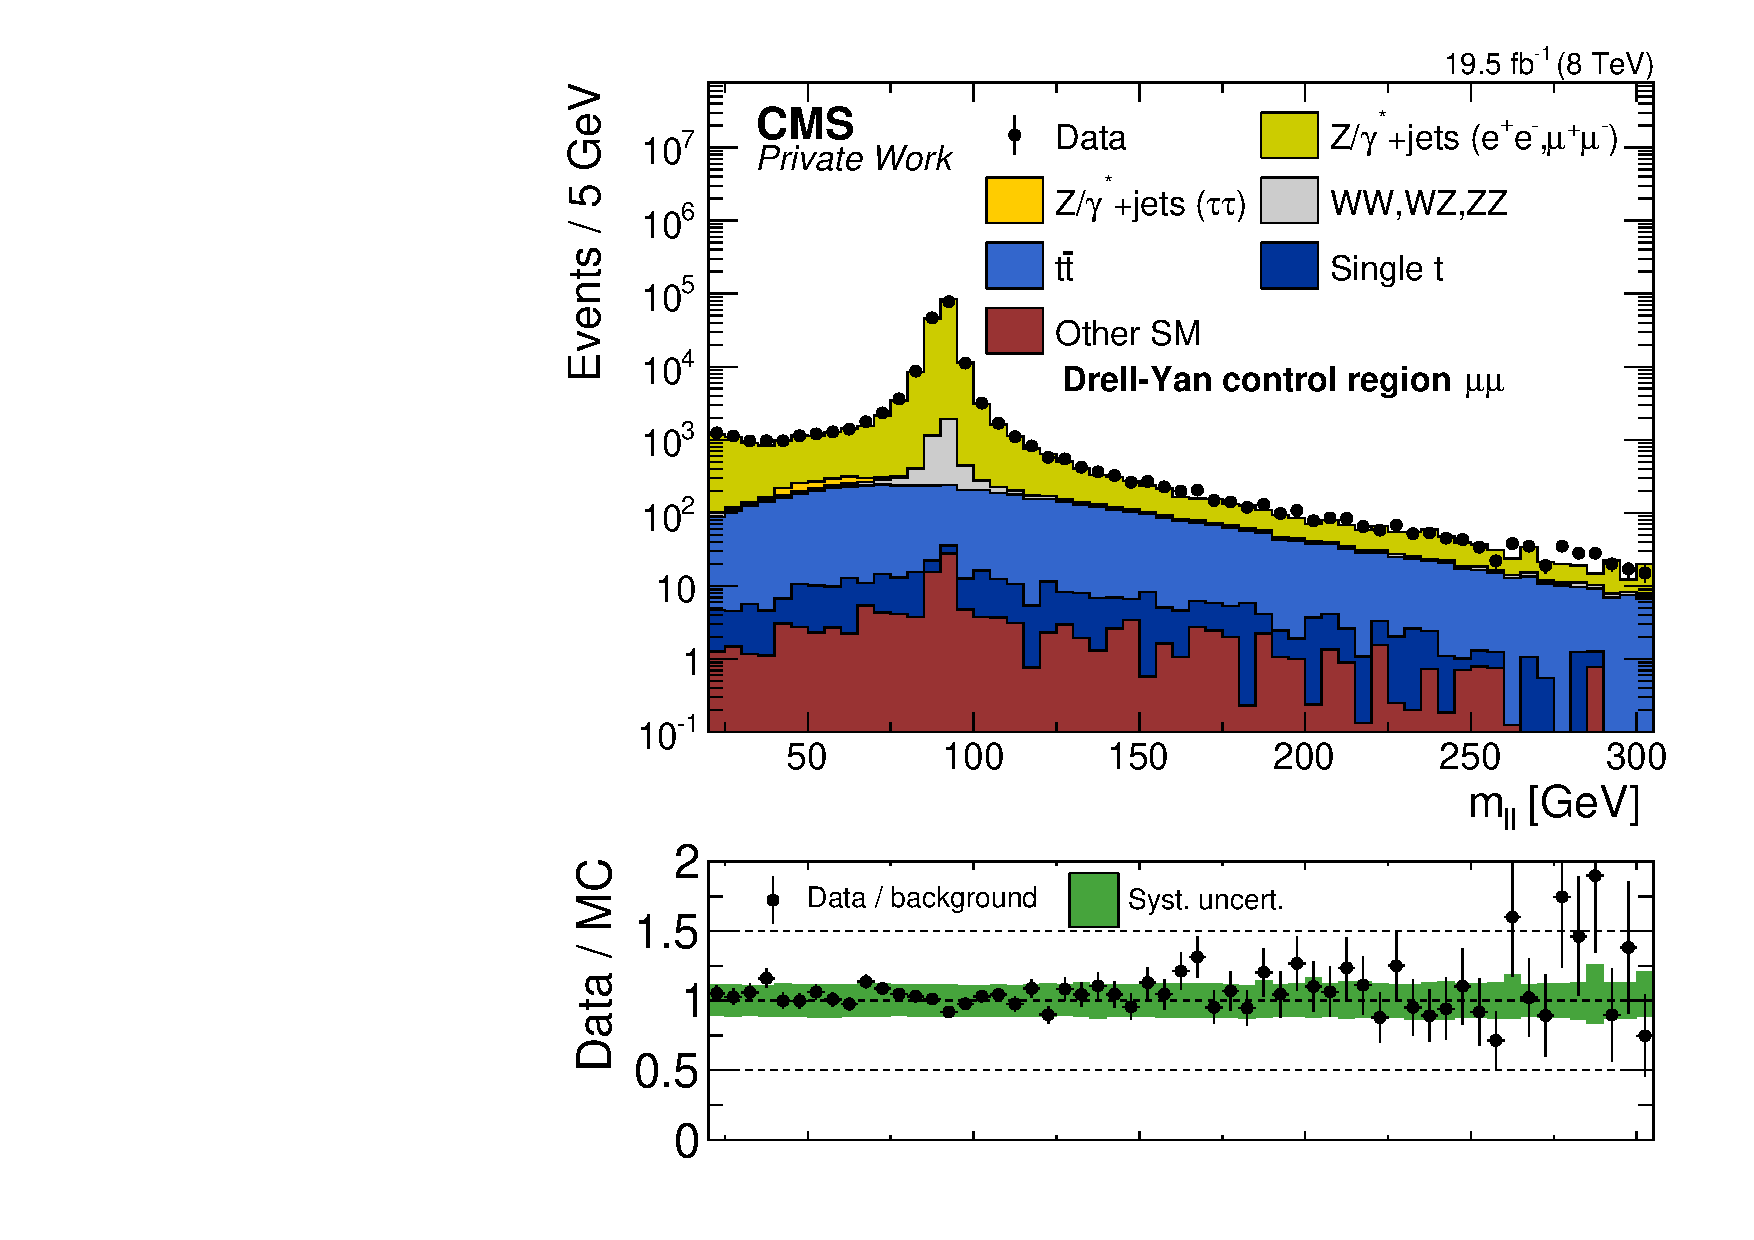
\includegraphics[width=\textwidth]{plots/BG/rmue/DrellYanControl_Mll_Full2012_MuMu_TopReweighted.pdf}
\end{minipage}
\begin{minipage}[t]{0.49\textwidth}
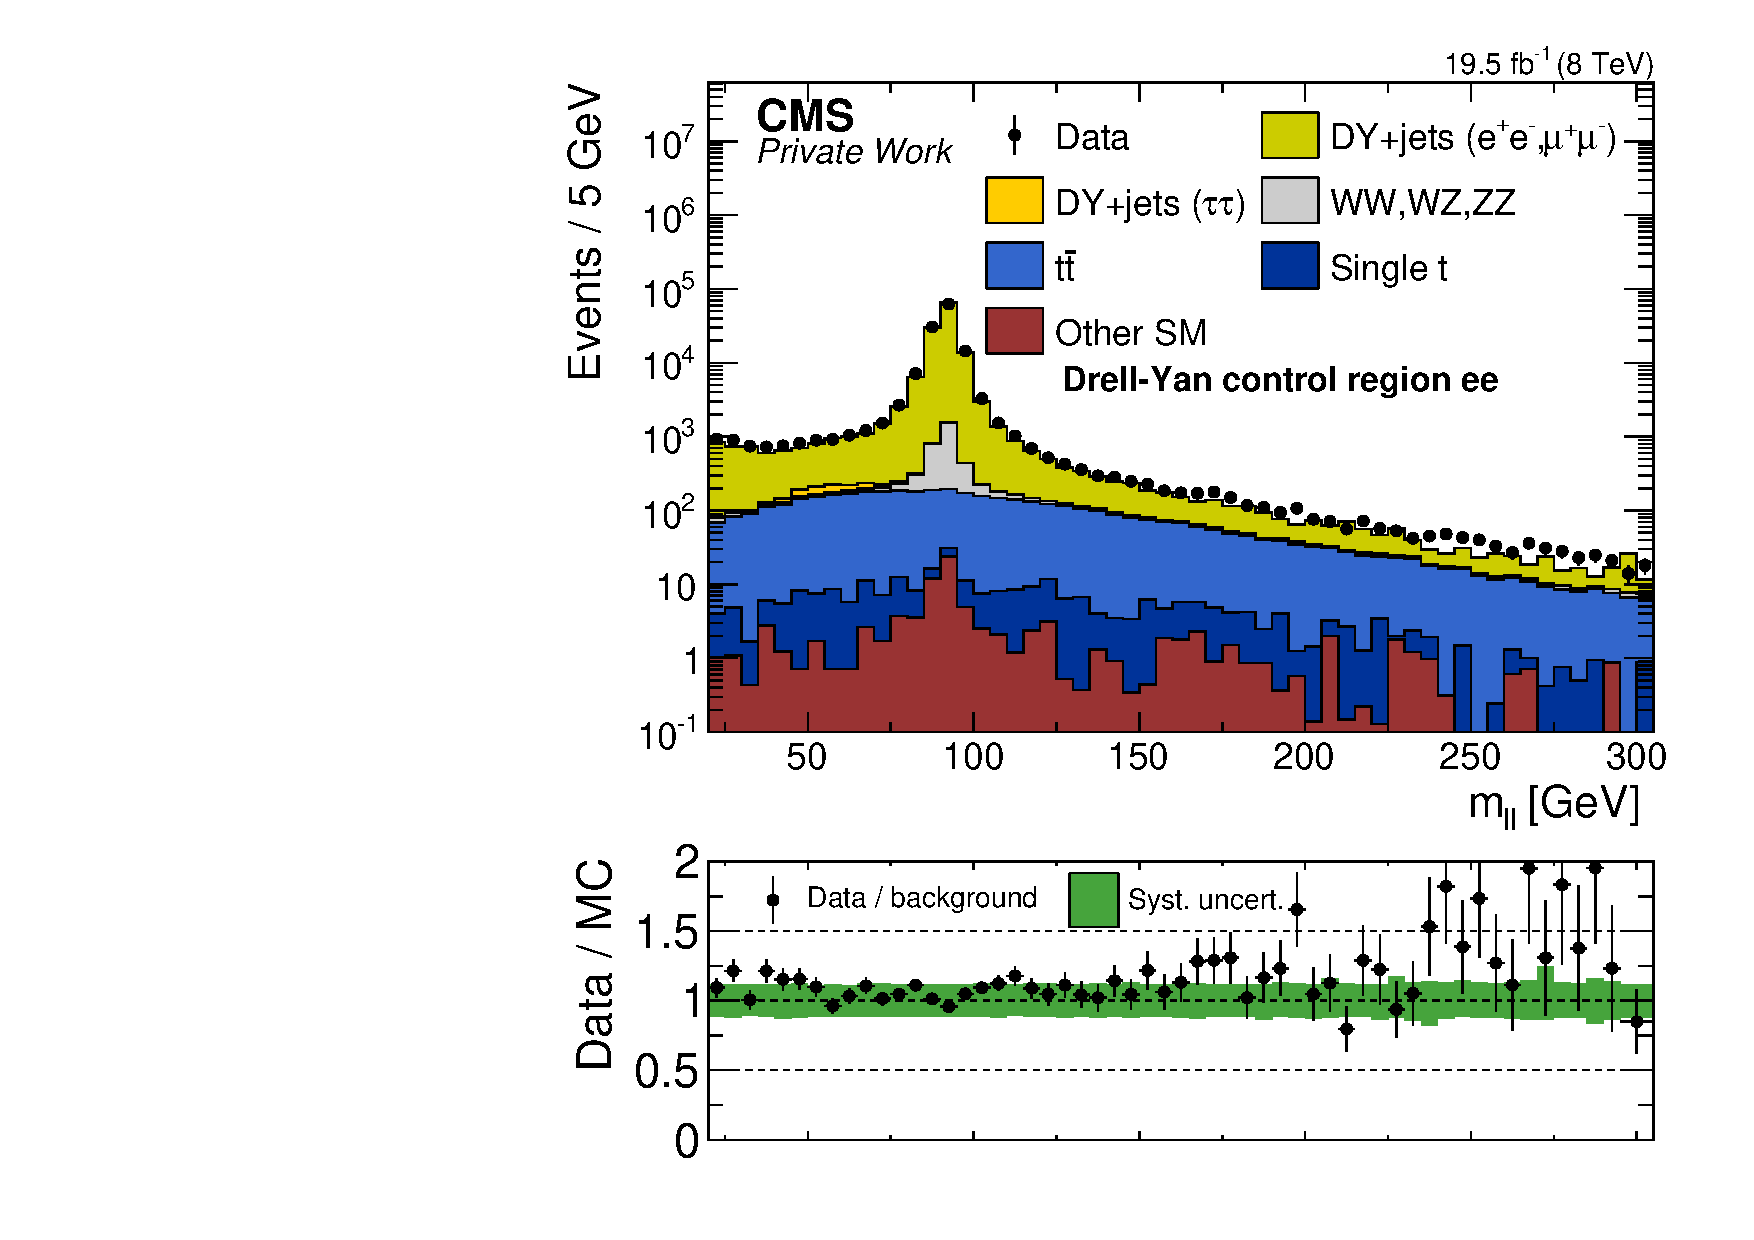
\includegraphics[width=\textwidth]{plots/BG/rmue/DrellYanControl_Mll_Full2012_EE_TopReweighted.pdf}
\end{minipage}
\caption{Distribution of \mll in the Drell-Yan control region for \MM events (left) and \EE events (right). The data is shown as the black dots, while the contributions from Standard Model processes, estimated from simulation, are shown as the stacked histograms.}
\label{fig:rmueMll}
\end{figure} 
The results of the calculation of \rmue are shown in Table~\ref{tab:rMuE}. Given are the observed yields for \MM and \EE events and the resulting value of \rmue with statistical and systematic uncertainties. In the central lepton selection, the \MM yield is about 18\% higher than the \EE yield. Similar results are observed on Drell-Yan simulation. For events with leptons in the forward region, a larger asymmetry between muons and electrons is observed, here the \MM yield is about 40\% higher than the \EE yield. 

\begin{table}[hbtp]
 \renewcommand{\arraystretch}{1.3}
 \setlength{\belowcaptionskip}{6pt}
 \centering
 \caption{Result of the calculation of \rmue. Shown are the observed event yields in the Drell--Yan control region for the central and forward lepton selection in the \EE and \MM channels and the resulting values of 
\rmue. The same quantaties derived from simulation are shown for comparison.}
  \label{tab:rMuE}
  \begin{tabular}{l| ccc }

    							& $N_{\mu\mu}$ &  $N_{ee}$ & $\rmue \pm \sigma_{\text{stat.}} \pm \sigma_{\text{syst.}}$ \\ 
    
    \hline
    							& \multicolumn{3}{c}{Central}  \\ 

    \hline
        Data       &  98284                   & 83035              &  1.09$\pm$0.01$\pm$0.11    \\

        MC       &  99719                   & 82035              &  1.10$\pm$0.00$\pm$0.11    \\

\hline
    							& \multicolumn{3}{c}{Forward}  \\ 

    \hline
        Data       &  62212                   & 44437              &  1.18$\pm$0.01$\pm$0.24    \\

        MC       &  66327                   & 45541              &  1.21$\pm$0.00$\pm$0.24    \\

  \end{tabular}
\end{table}



The systematic uncertainties assigned to the measured values of \rmue are 10\% for the central and 20\% for the forward lepton selection. These values are obtained by studying the dependency of \rmue on relevant observables. These are on the one hand properties of the lepton pairs, while on the other hand event properties as the jet multiplicity and \MET are studied to ensure the applicability of \rmue in the signal region. The dependencies of \rmue on \mll, \MET, and $N_{jets}$ are shown in Figure~\ref{fig:rmueDependencies}. Some dependency is observed in the case of \mll, where the values are higher for low \mll below the Z peak. This can be traced back to a dependency on the \pt of the leptons, where the efficiencies for muons have sharper turnons compared to electrons. In data, there is a strong effect visible around the Z peak for forward leptons. This is caused by a systematic shift of the position of the Z peak between electron and muons and is not a general property of \rmue, as is evident from the comparison with $t\bar{t}$ simulation shown in the upper right of Figure~\ref{fig:rmueDependencies}. No strong dependencies can be observed for \MET and $N_{jets}$ within the statistical uncertainties. All observed deviations from the central values are covered by the systematic uncertainties assigned to the measurement. Further information on the dependency studies can be found in Appendix~\ref{app:rmue}.
\begin{figure}[htbp]
\centering
\begin{minipage}[t]{0.49\textwidth}
  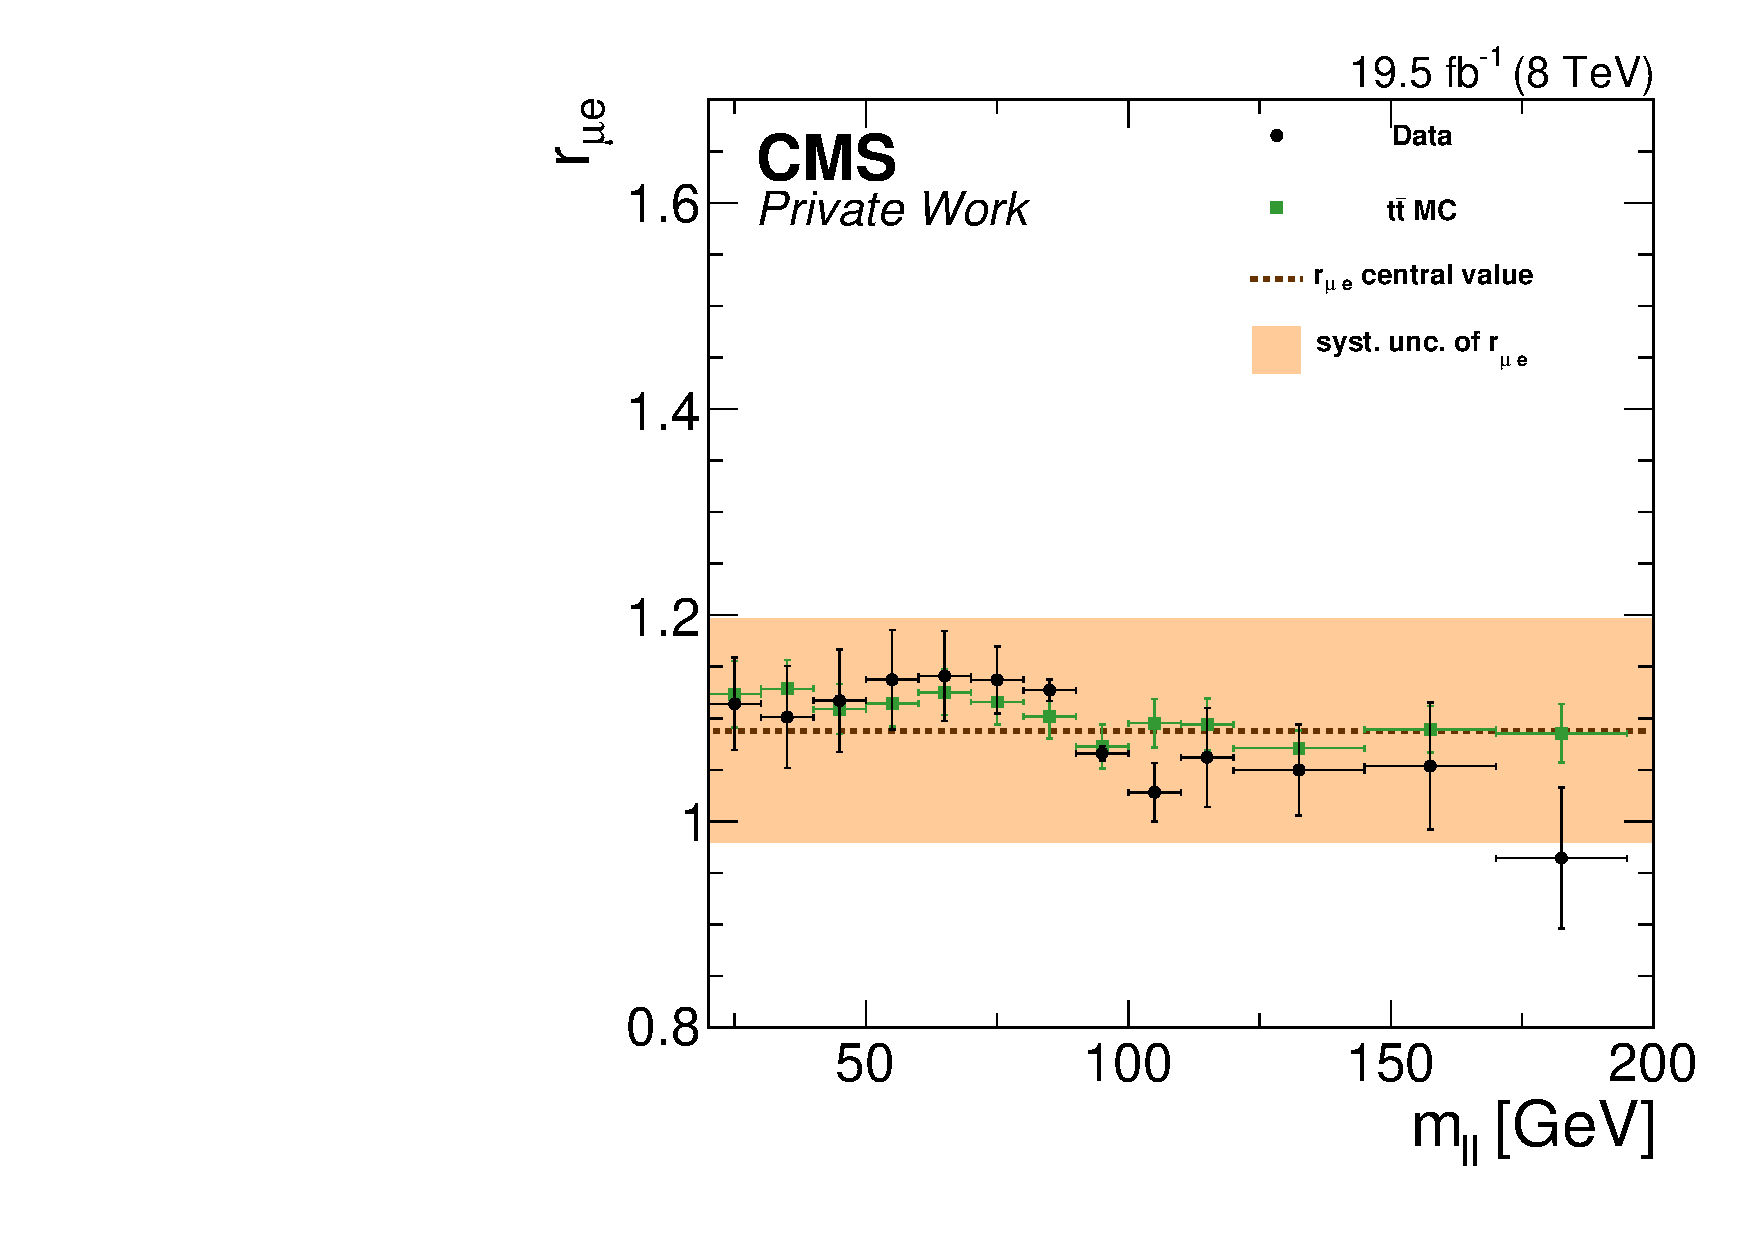
\includegraphics[width=\textwidth]{plots/BG/rmue/rMuE_ZPeakControlCentral_Full2012_Mll_None.pdf}
\end{minipage}
\begin{minipage}[t]{0.49\textwidth}
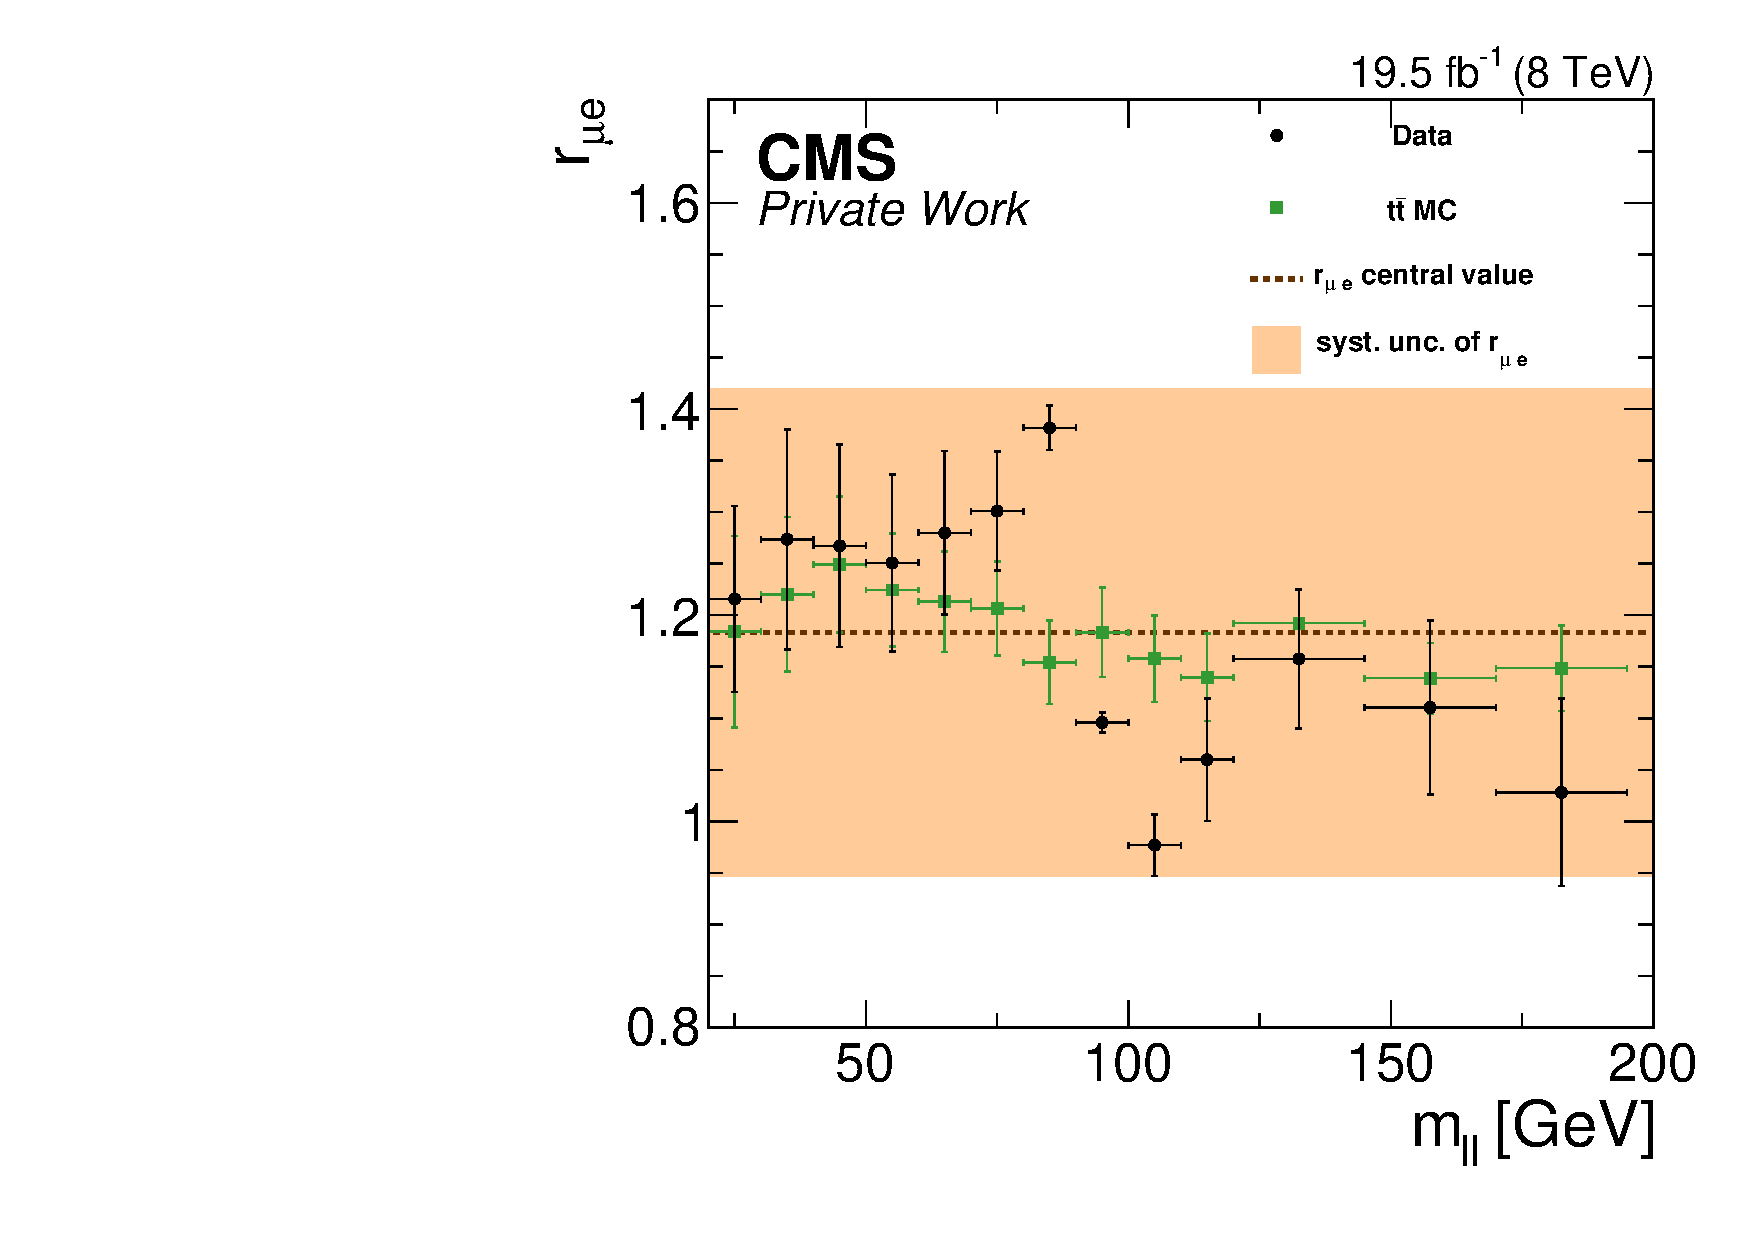
\includegraphics[width=\textwidth]{plots/BG/rmue/rMuE_ZPeakControlForward_Full2012_Mll_None.pdf}
\end{minipage}
\begin{minipage}[t]{0.49\textwidth}
  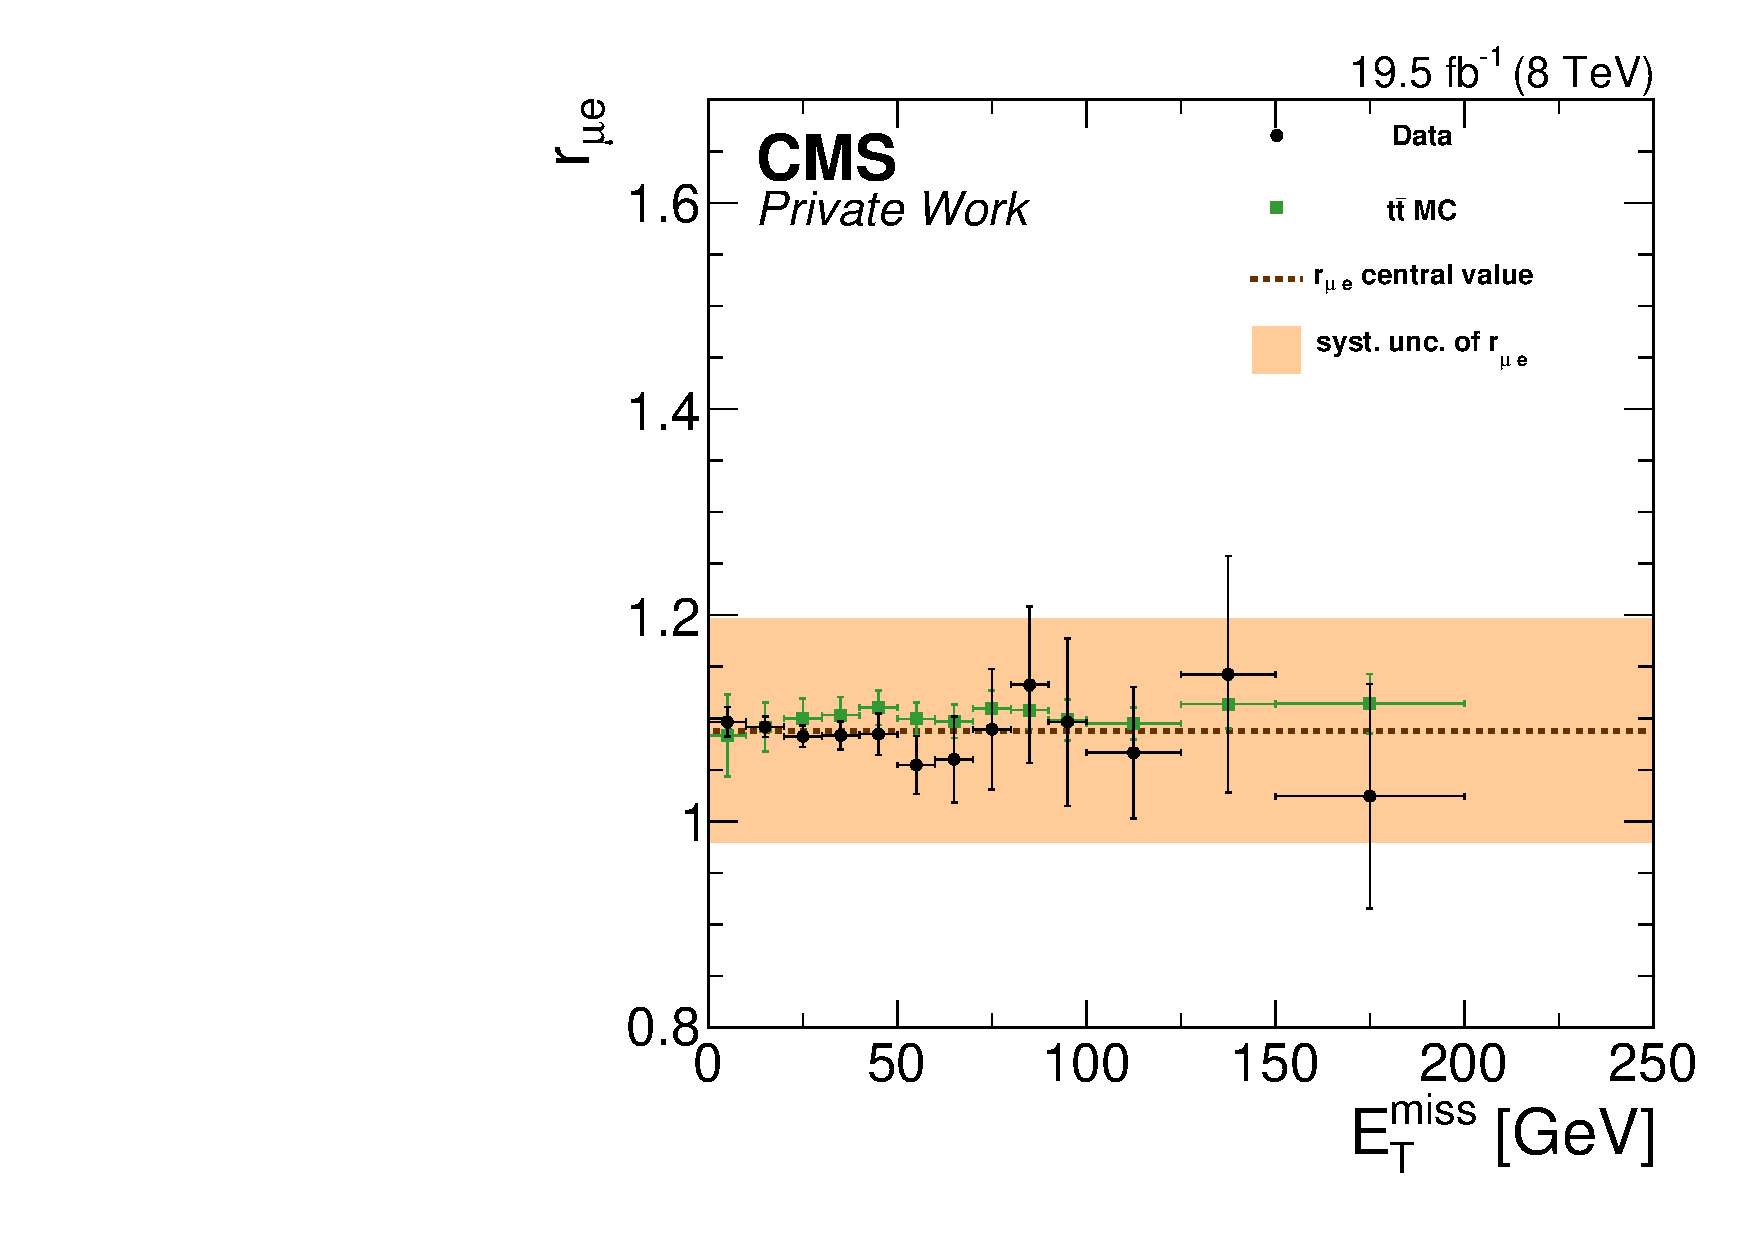
\includegraphics[width=\textwidth]{plots/BG/rmue/rMuE_ZPeakControlCentral_Full2012_MET_None.pdf}
\end{minipage}
\begin{minipage}[t]{0.49\textwidth}
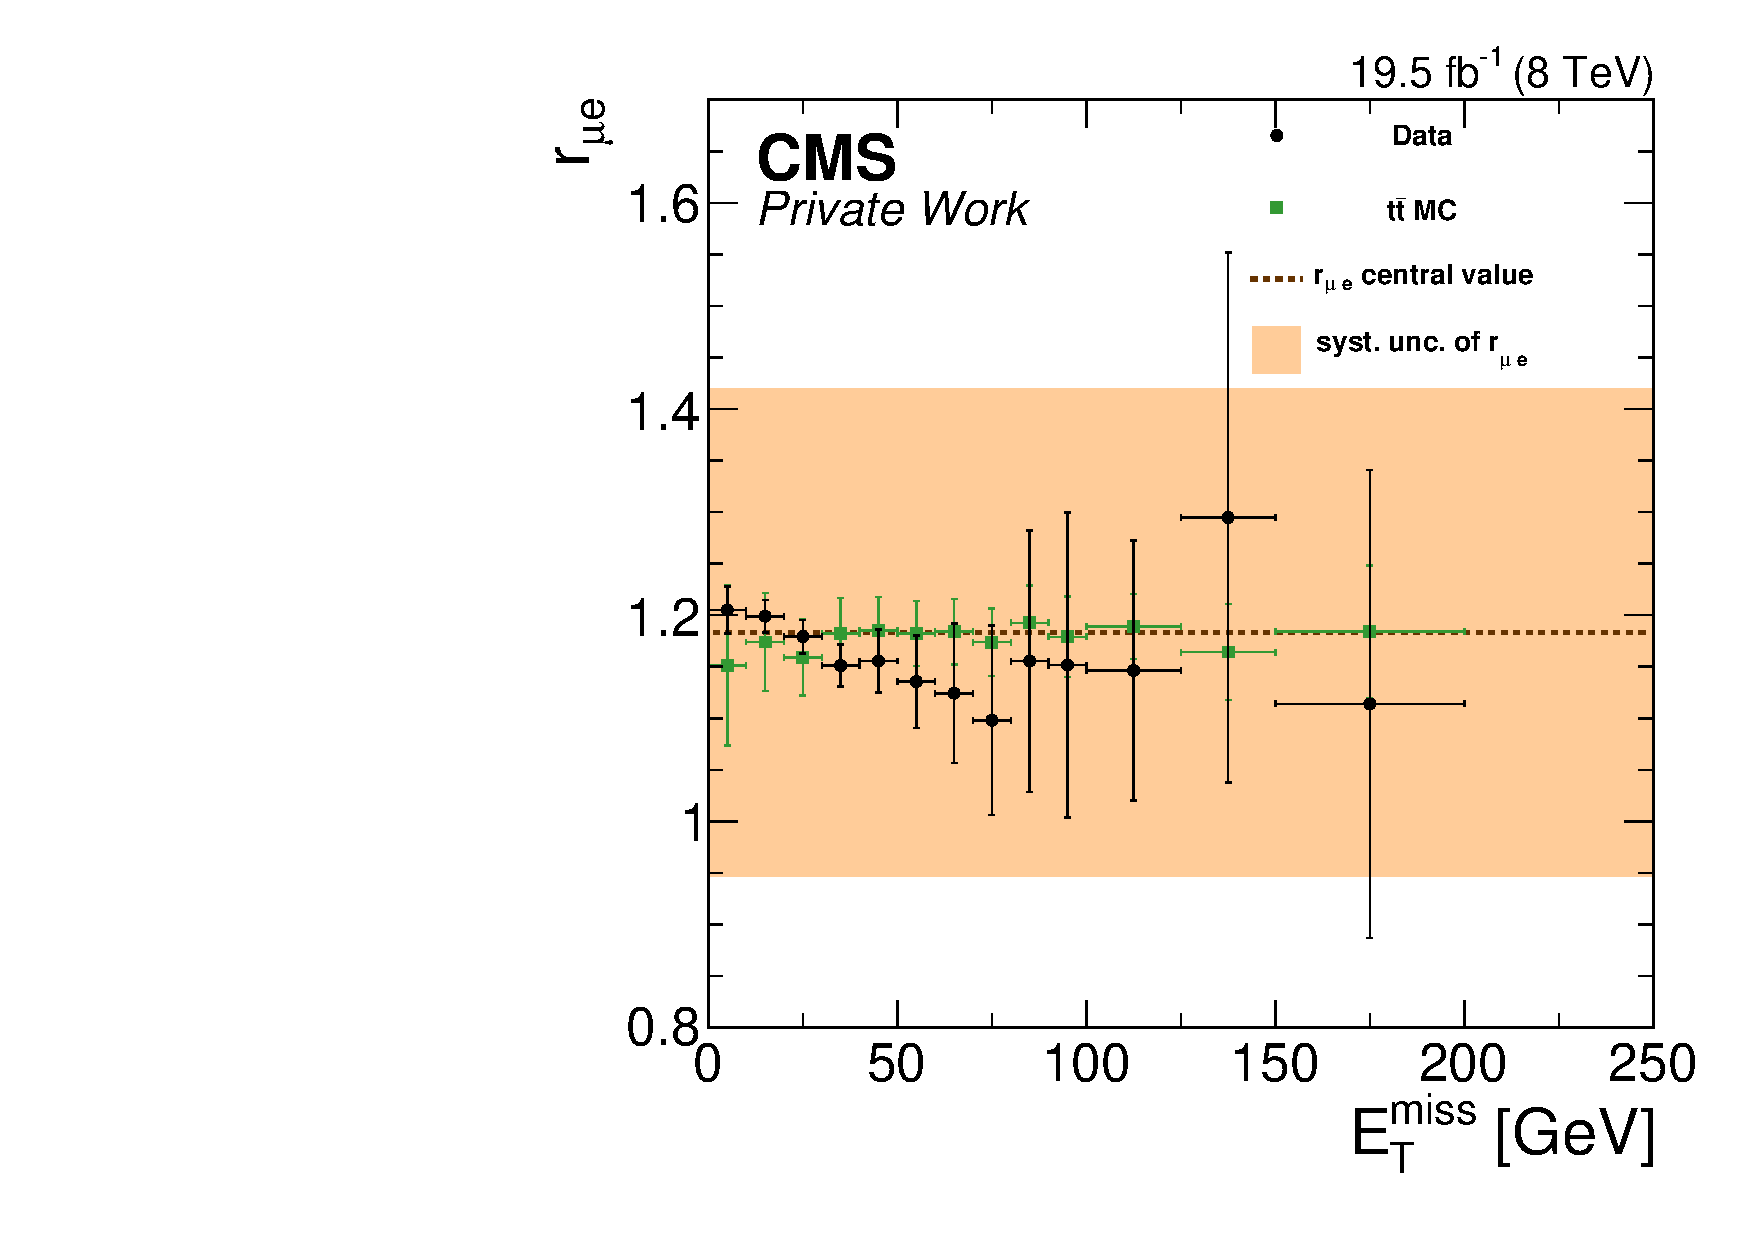
\includegraphics[width=\textwidth]{plots/BG/rmue/rMuE_ZPeakControlForward_Full2012_MET_None.pdf}
\end{minipage}
\begin{minipage}[t]{0.49\textwidth}
  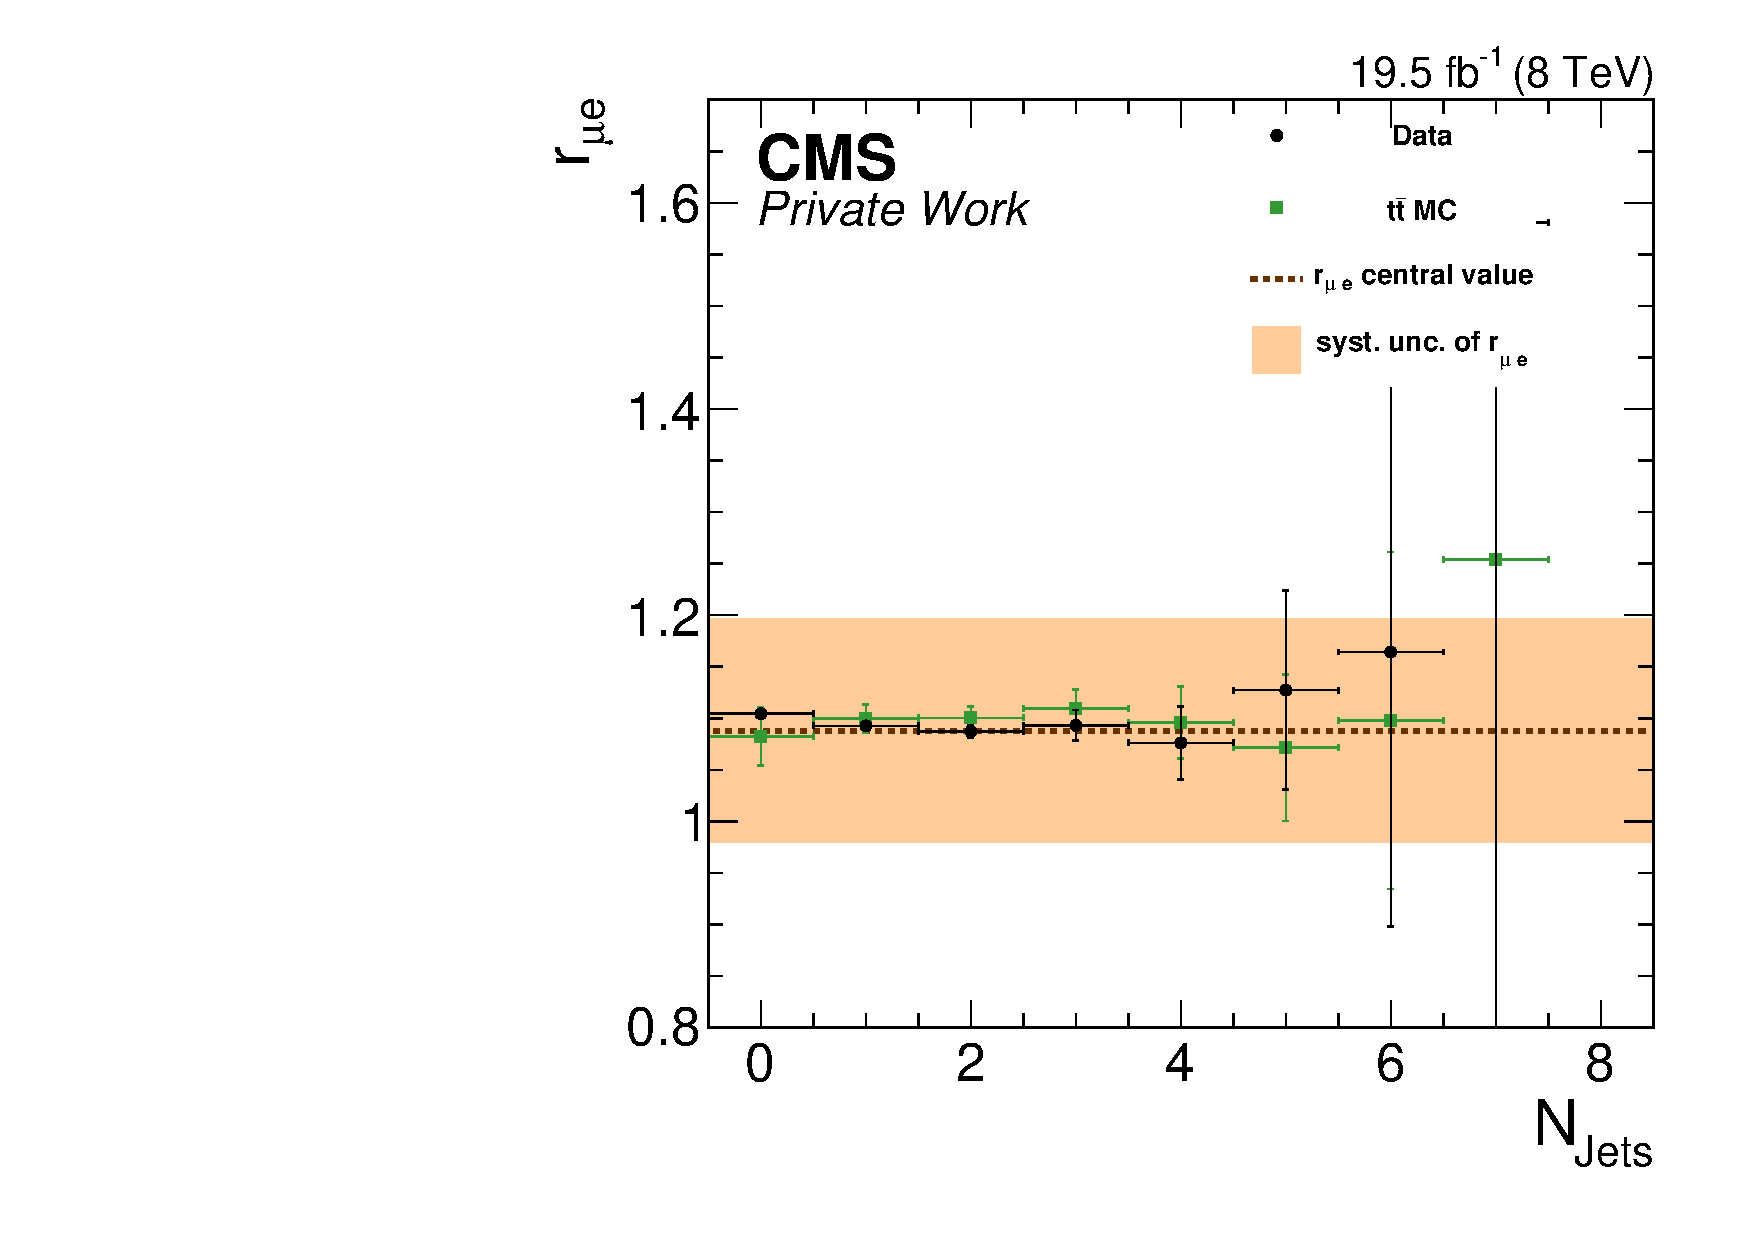
\includegraphics[width=\textwidth]{plots/BG/rmue/rMuE_ZPeakControlCentral_Full2012_NJets_None.pdf}
\end{minipage}
\begin{minipage}[t]{0.49\textwidth}
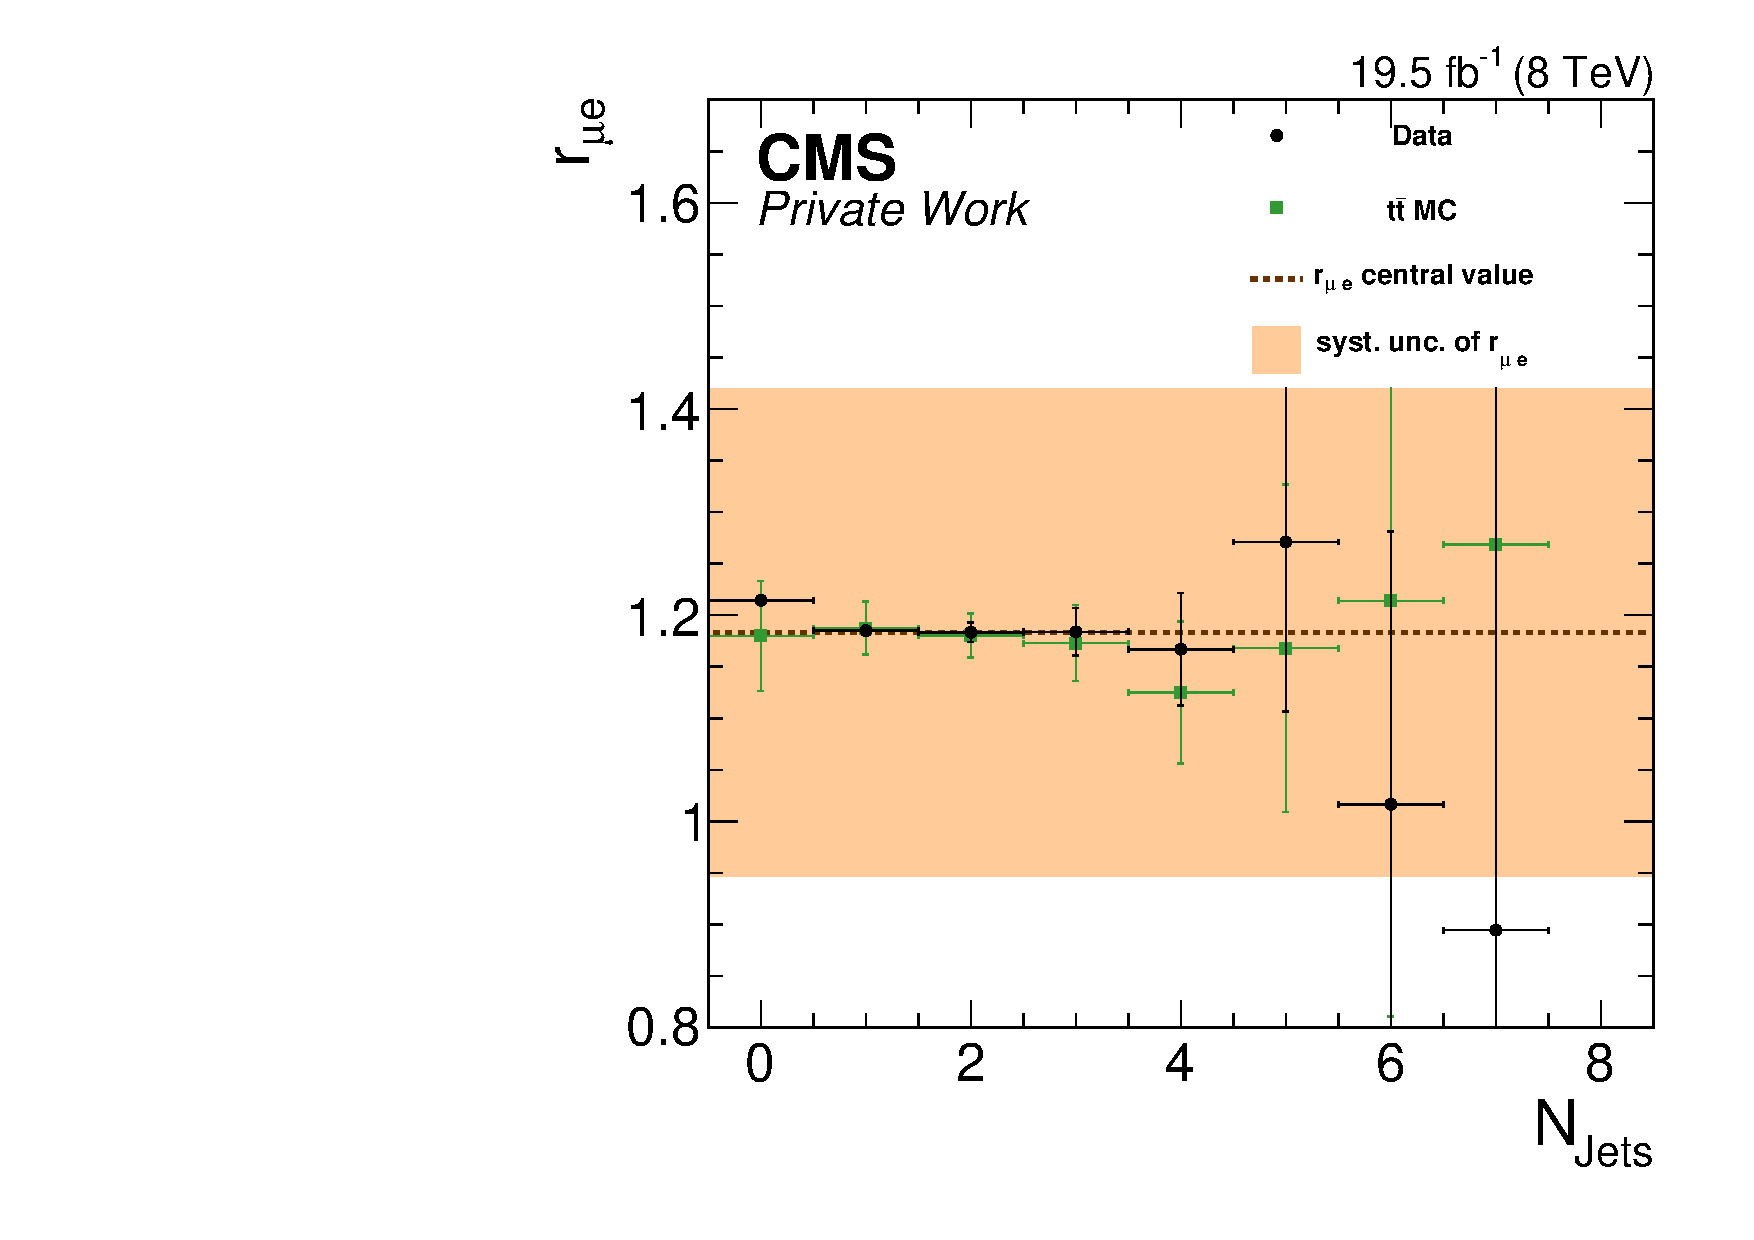
\includegraphics[width=\textwidth]{plots/BG/rmue/rMuE_ZPeakControlForward_Full2012_NJets_None.pdf}
\end{minipage}
\caption{Dependencies of \rmue on \mll (top), \MET (middle), and $N_{jets}$ (bottom) for the central (left) and forward (right) lepton selection. The results on data are shown in black while $t\bar{t}$ simulation is shown in green. The central value is shown as a brown dashed line while the systematic uncertainty is shown as an orange band.}
\label{fig:rmueDependencies}
\end{figure} 
\subsubsection{Measurement of \RT}
\label{sec:triggerEffs}
The trigger efficiencies are measured utilizing an event sample collected with PF $H_T$ triggers. Lepton pairs corresponding to the flavour combination of the trigger in question are selected. To ensure that only correctly reconstructed events are considered in the calculation of the trigger efficiencies, the events are required to have $H_T > \unit{200}{\giga\electronvolt}$, which corresponds to the lowest threshold applied in one of the PF $H_T$ trigger. To ensure that the factorization method is performed on event samples complete orthogonal to the signal region and the $t\bar{t}$ enriched control region, events with $N_{jets} \geq 2$ and $\MET > \unit{100}{\giga\electronvolt}$ are rejected. As the offline lepton selection has more strict requirements compared to the one applied at HLT level, the dilepton triggers should have accepted all these events. The trigger efficiency is therefore defined as the ratio of accepted events by the total number of events:
\begin{equation}
\epsilon_{ll}^T = \frac{N_{events}(\text{PF }H_T\text{trigger} \cap \text{dilepton selection} \cap \text{dilepton trigger})}{N_{events}(\text{PF }H_T\text{trigger} \cap \text{dilepton selection})}.
\end{equation}
In the case of \MM and OF events, two triggers are used in the event selection. Therefore their combined efficiency is measured, requesting the logical OR of both. The resulting efficiencies are summarized in Table~\ref{tab:triggerEffs}, separately for the central and forward lepton selection. The trigger efficiencies for \EE and \MM are about 97\% in both the central and forward selection. The efficiency for OF events is lower, about 95\% in the central and 90\% in the forward selection. This shows how the flavour symmetry is broken at trigger level by the inclusion of the \verb+HLT_Mu17_TkMu8+ trigger, which recovers efficiency for the trailing muon leg of the trigger and is not present in the OF triggers.   

\begin{table}[hbp] \caption{Trigger efficiencies measured using \HT baseline trigger. The results are shown for the central and forward regions separately.} 
\centering 
\renewcommand{\arraystretch}{1.2} 
\begin{tabular}{l|c|c|c|c|c|c}     

 & nominator & denominator & $\epsilon_{\ell\ell}^{T} \pm \sigma_{\text{stat}}$ &  nominator & denominator & $\epsilon_{\ell\ell}^{T} \pm \sigma_{\text{stat}}$  \\ 
\hline

&\multicolumn{6}{c}{Data} \\
\hline
&  \multicolumn{3}{c|}{Central } & \multicolumn{3}{c}{ Forward }\\
\hline
ee & 3592 & 3692 & 0.973$\pm$0.003 & 954 & 980 & 0.973$\pm$0.006 \\
$\mu\mu$ & 1375 & 1420 & 0.968$\pm$0.005 & 547 & 566 & 0.966$\pm$0.009 \\
e$\mu$ & 493 & 521 & 0.946$\pm$0.012 & 102 & 114 & 0.895$\pm$0.037 \\
 
 
\hline

& \multicolumn{6}{c}{MC} \\
\hline
&  \multicolumn{3}{c|}{Central } & \multicolumn{3}{c}{ Forward } \\
\hline 
ee & 2912.8 & 2994.6 & 0.973$\pm$0.001 & 943.0 & 969.9 & 0.972$\pm$0.001 \\
$\mu\mu$ & 3241.6 & 3287.9 & 0.986$\pm$0.001 & 1141.6 & 1183.4 & 0.965$\pm$0.001 \\
e$\mu$ & 6279.1 & 6523.1 & 0.963$\pm$0.001 & 2138.8 & 2249.0 & 0.951$\pm$0.001 \\
    
    \hline 
\end{tabular}  
\label{tab:EffValues_Seperated}
\end{table}	

To asses the systematic uncertainties of the trigger efficiency measurement, potential biases due to the choice of the orthogonal trigger  are studied on simulation, using dileptonic $t\bar{t}$ events. On simulation the efficiency can be measured without the requirement of the PF $H_T$ triggers, as no trigger is needed to select the events. The ratio of this true trigger efficiencies to those measured with the PF $H_T$ triggers as a function of \mll is shown in Figure~\ref{fig:triggerEffBias}, separately for SF and OF events. In both cases all deviations from one are in the order of 0.1\% and well compatible with it inside the statistical uncertainties. No bias of the efficiency measurement due to the PF $H_T$ triggers is observed and therefore no systematic uncertainty due to this choice is assigned to the measurement.
\begin{figure}
\begin{center}
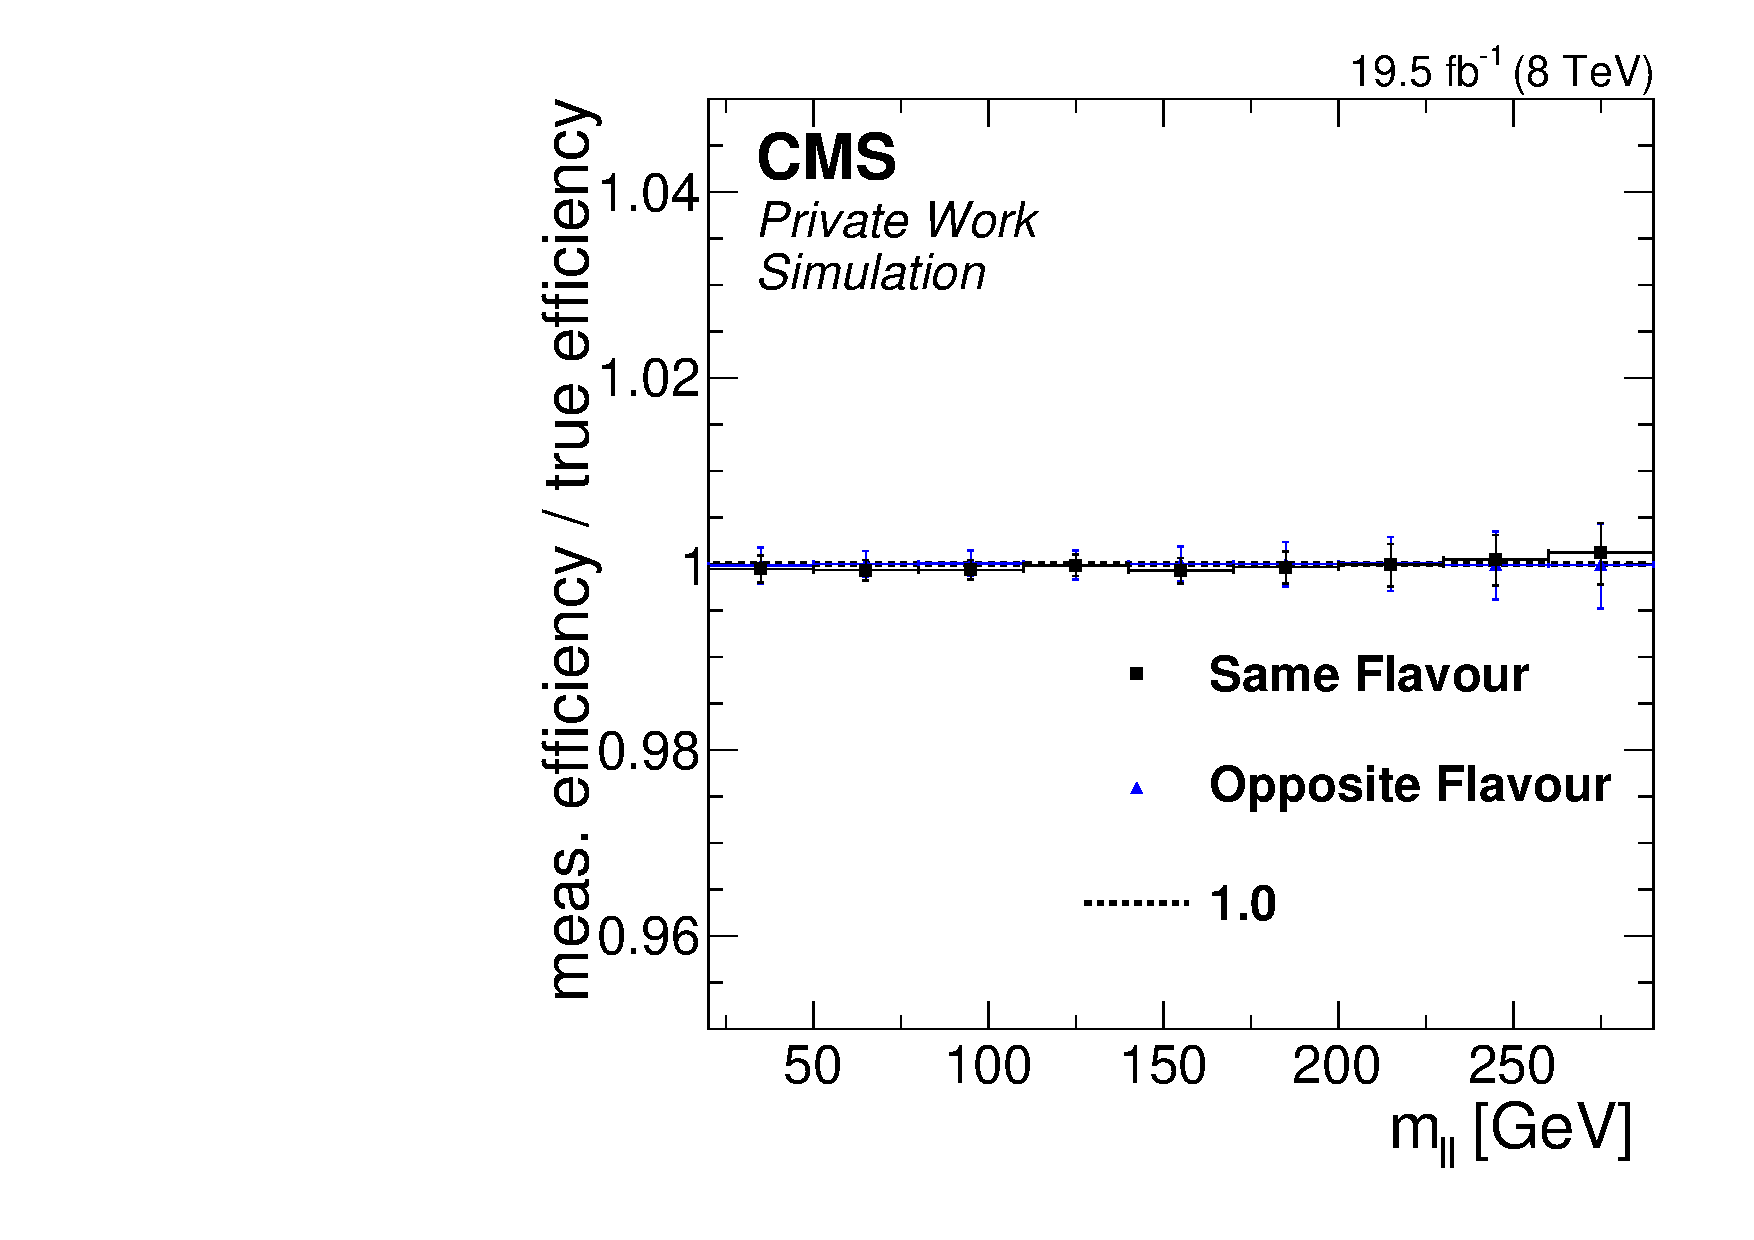
\includegraphics[scale=0.35]{plots/BG/trigger/Triggereff_AlphaTSyst_PFHT_HighHTExclusive_Full2012_Mll_None.pdf}
\caption{Ratio of true trigger efficiencies to those calculated using the PF $H_T$ triggers separately for SF and OF events.}
\label{fig:triggerEffBias}
\end{center}
\end{figure}
The turnon of the triggers at low lepton \pt is of particular interest because asymmetries between the lepton flavours are more likely to occur in this difficult environment. The dependence of the trigger efficiency on the \pt of the trailing lepton can be studied using datasets trigger by single lepton triggers. Triggers with \pt thresholds of $\unit{24(27)}{\giga\electronvolt}$ for muons (electrons) are available. These thresholds are relatively low for single lepton triggers, resulting in very strict selection criteria having to be applied on HLT level. Dilepton events are selected in which the leading lepton can be matched  geometrically to the trigger object that fired the single lepton trigger. The trailing lepton is matched to trigger objects that have fired the trailing leg of the dilepton trigger. The efficiency is defined as the number of events in which such a match can be found to the total number of dilepton events. The resulting efficiency curves are shown in Figure~\ref{fig:triggerEffTrailing} for five different trailing lepton trigger legs and combining the central and forward selection. It can be seen that the efficiency for trailing electrons are virtually the same for the dielectron and OF triggers (black and light blue markers). The same is true for trailing muons in the dimuon and OF triggers (brown and dark blue markers). However, the efficiency for trailing muons in the \verb+HLT_Mu17_TkMu8+ trigger is significantly higher than those in the trigger paths not using the tracker information, as expected. Trailing muons have a much sharper turnon than trailing electrons, being fully efficient already at a \pt of $\unit{10}{\giga\electronvolt}$. For electrons the plateau is reached only above $\unit{\approx 30}{\giga\electronvolt}$. The turnon is steeper for trailing electrons in the dielectron trigger compared to those in the OF trigger, resulting in an increased deviation from flavour symmetry below $\unit{20}{\giga\electronvolt}$. As in the design of the analysis the precision and stability of the background prediction was given priority over lepton acceptance, events with trailing leptons in this \pt range are rejected.  
\begin{figure}
\begin{center}
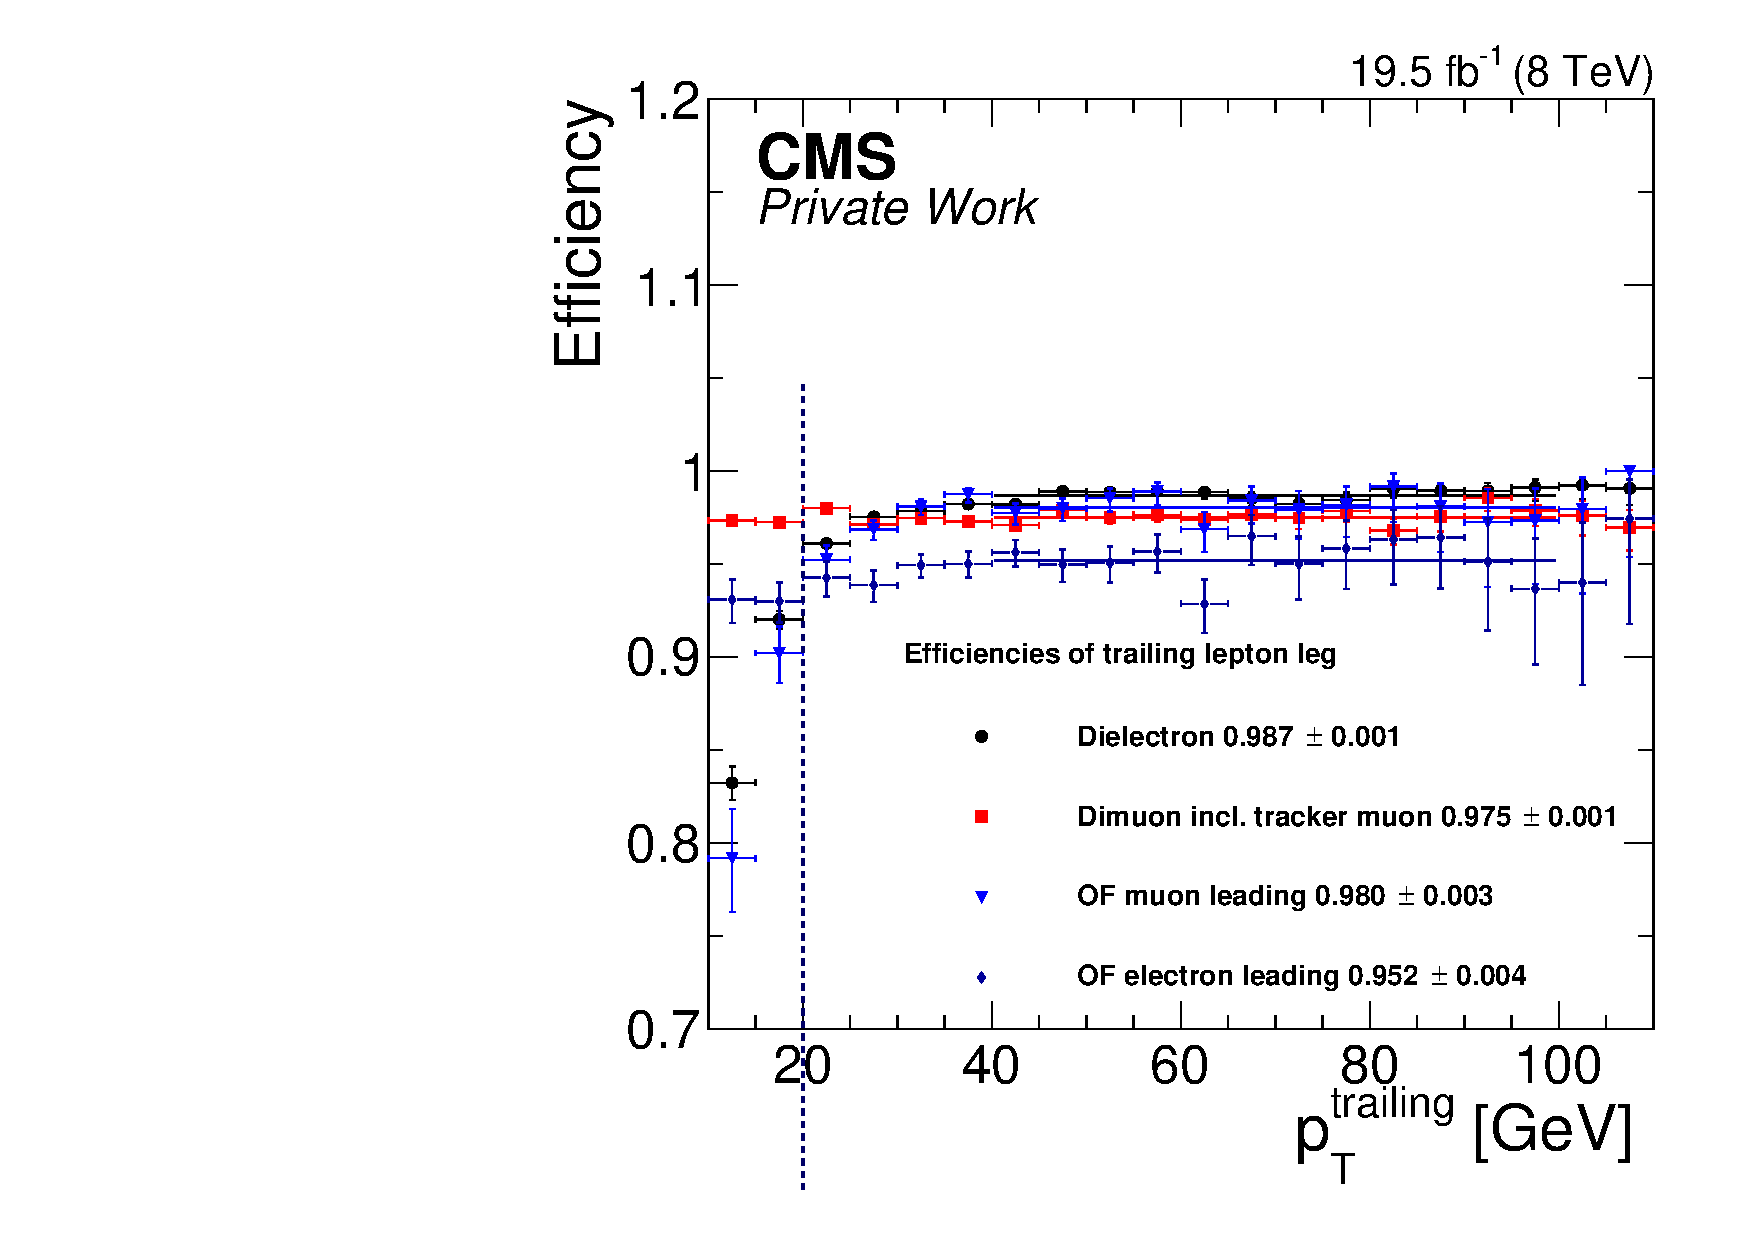
\includegraphics[scale=0.35]{plots/BG/trigger/Triggereff_SingleLepton_HighHTExclusive_Full2012_TrailingPt_leadingPt30Single.pdf}
\caption{Ratio of true trigger efficiencies to those calculated using the PF $H_T$ triggers separately for SF and OF events.}
\label{fig:triggerEffTrailing}
\end{center}
\end{figure} 
To asses the systematic uncertainties of the trigger efficiency measurement, the dependency of $R_T$ as used in the calculation of \Rsfof on different observables is tested. Here a dataset not triggered by $\alpha_T$ triggers is used, as the PF $H_T$ triggers do not provide enough events for these studies. A 5\% systematic uncertainty is assigned to each trigger efficiency, resulting in an uncertainty of 6.4\% on $R_T$, covering all observed deviations from the the measured value of $R_T$ within the statistical uncertainties, as shown in Figure\ref{fig:RTDependencies}. Studies of further variables can be found in Appendix~\ref{app:RT}
\begin{figure}[htbp]
\centering
\begin{minipage}[t]{0.49\textwidth}
  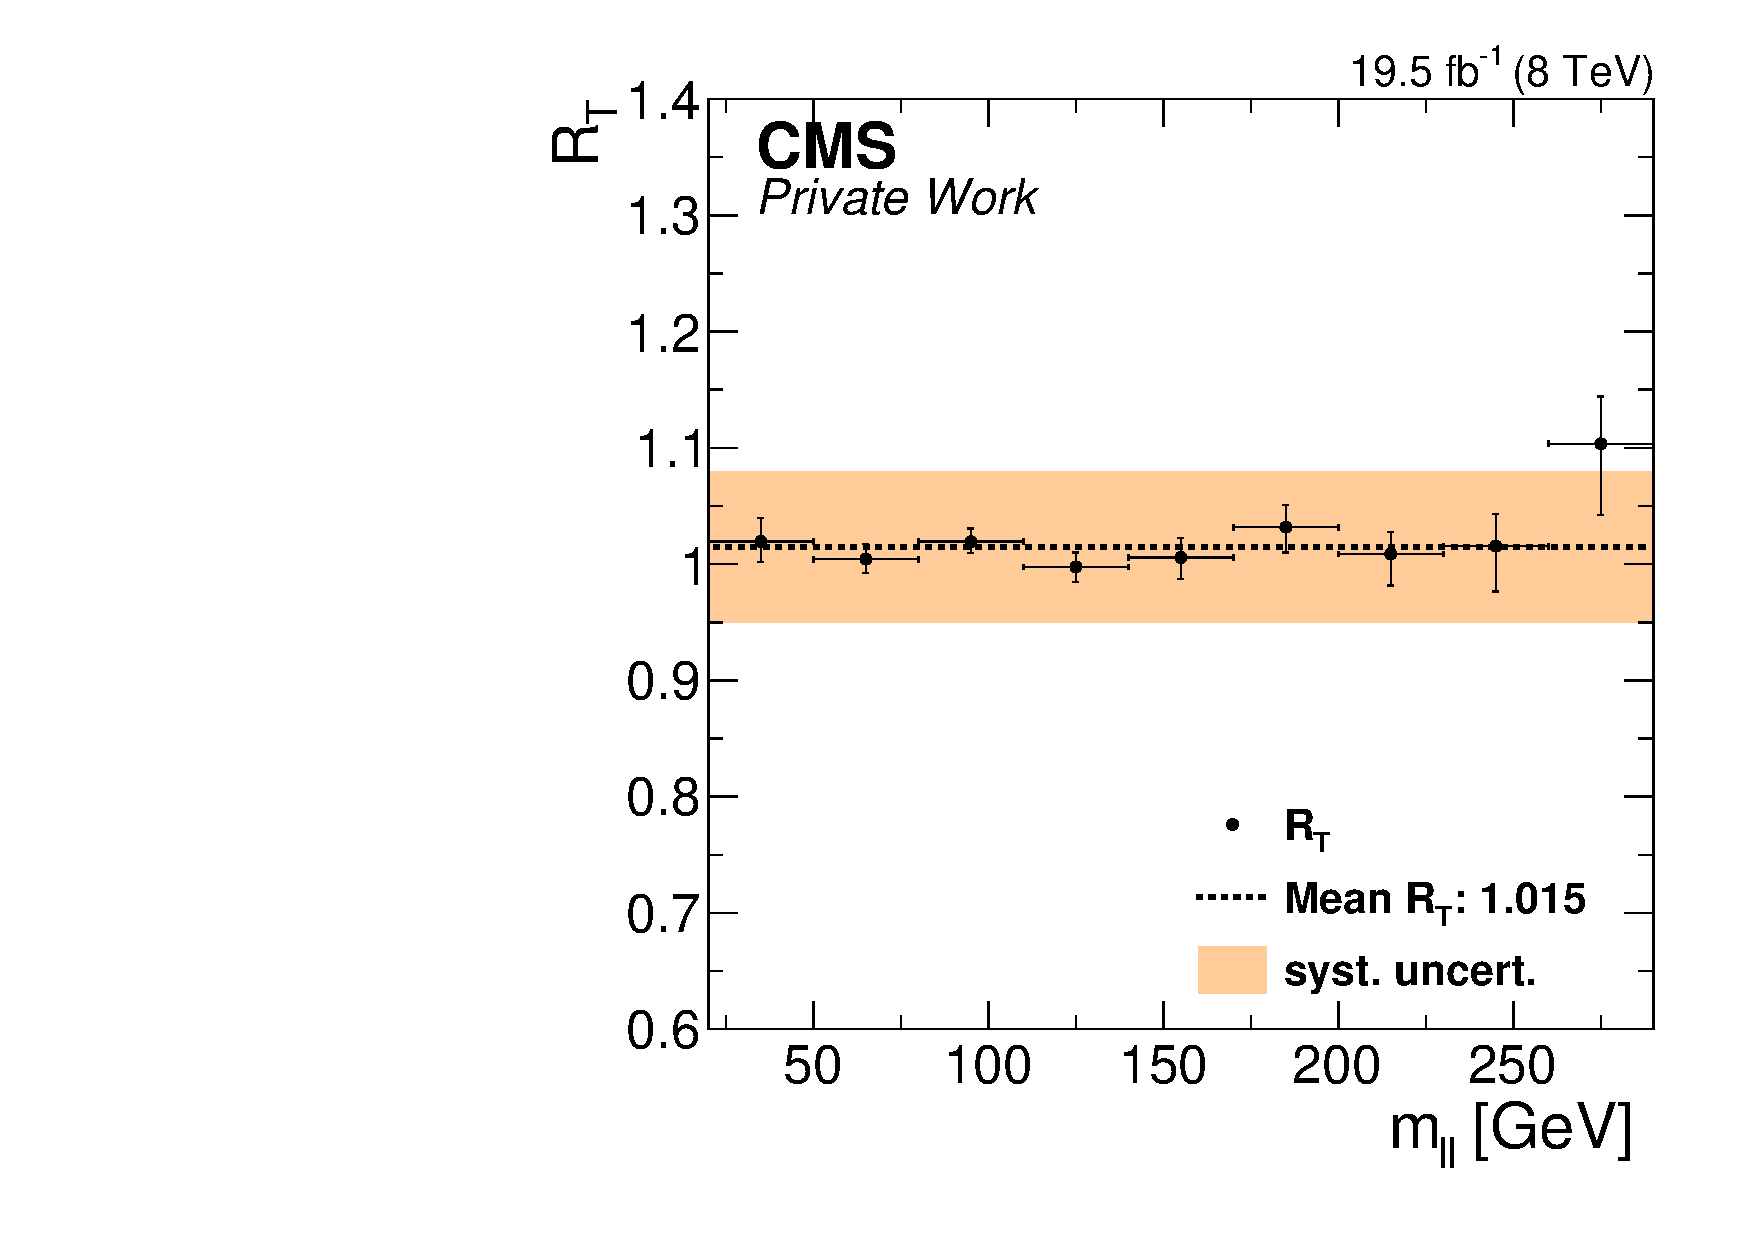
\includegraphics[width=\textwidth]{plots/BG/trigger/Triggereff_SFvsOF_Syst_AlphaT_HighHTExclusiveCentral_Full2012_Mll_None.pdf}
\end{minipage}
\begin{minipage}[t]{0.49\textwidth}
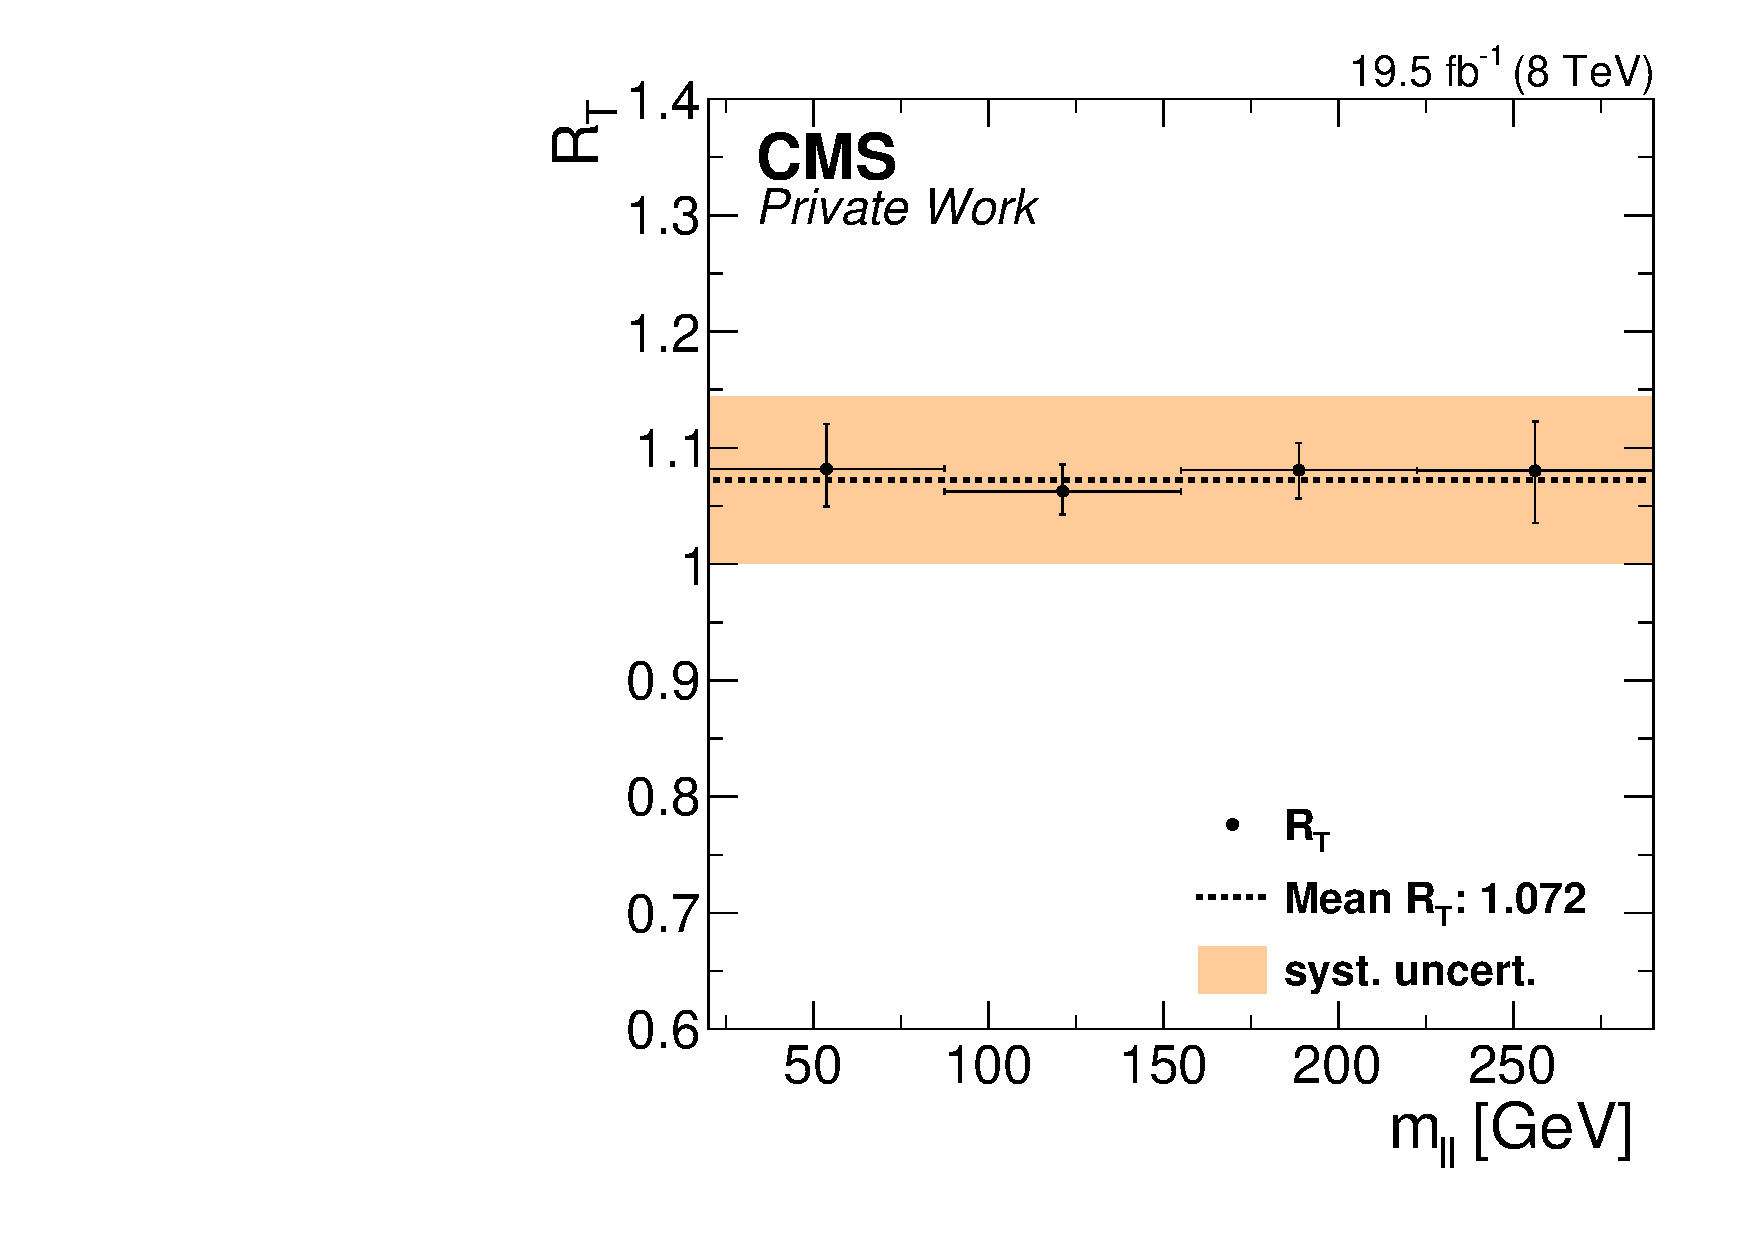
\includegraphics[width=\textwidth]{plots/BG/trigger/Triggereff_SFvsOF_Syst_AlphaT_HighHTExclusiveForward_Full2012_Mll_None.pdf}
\end{minipage}
\begin{minipage}[t]{0.49\textwidth}
  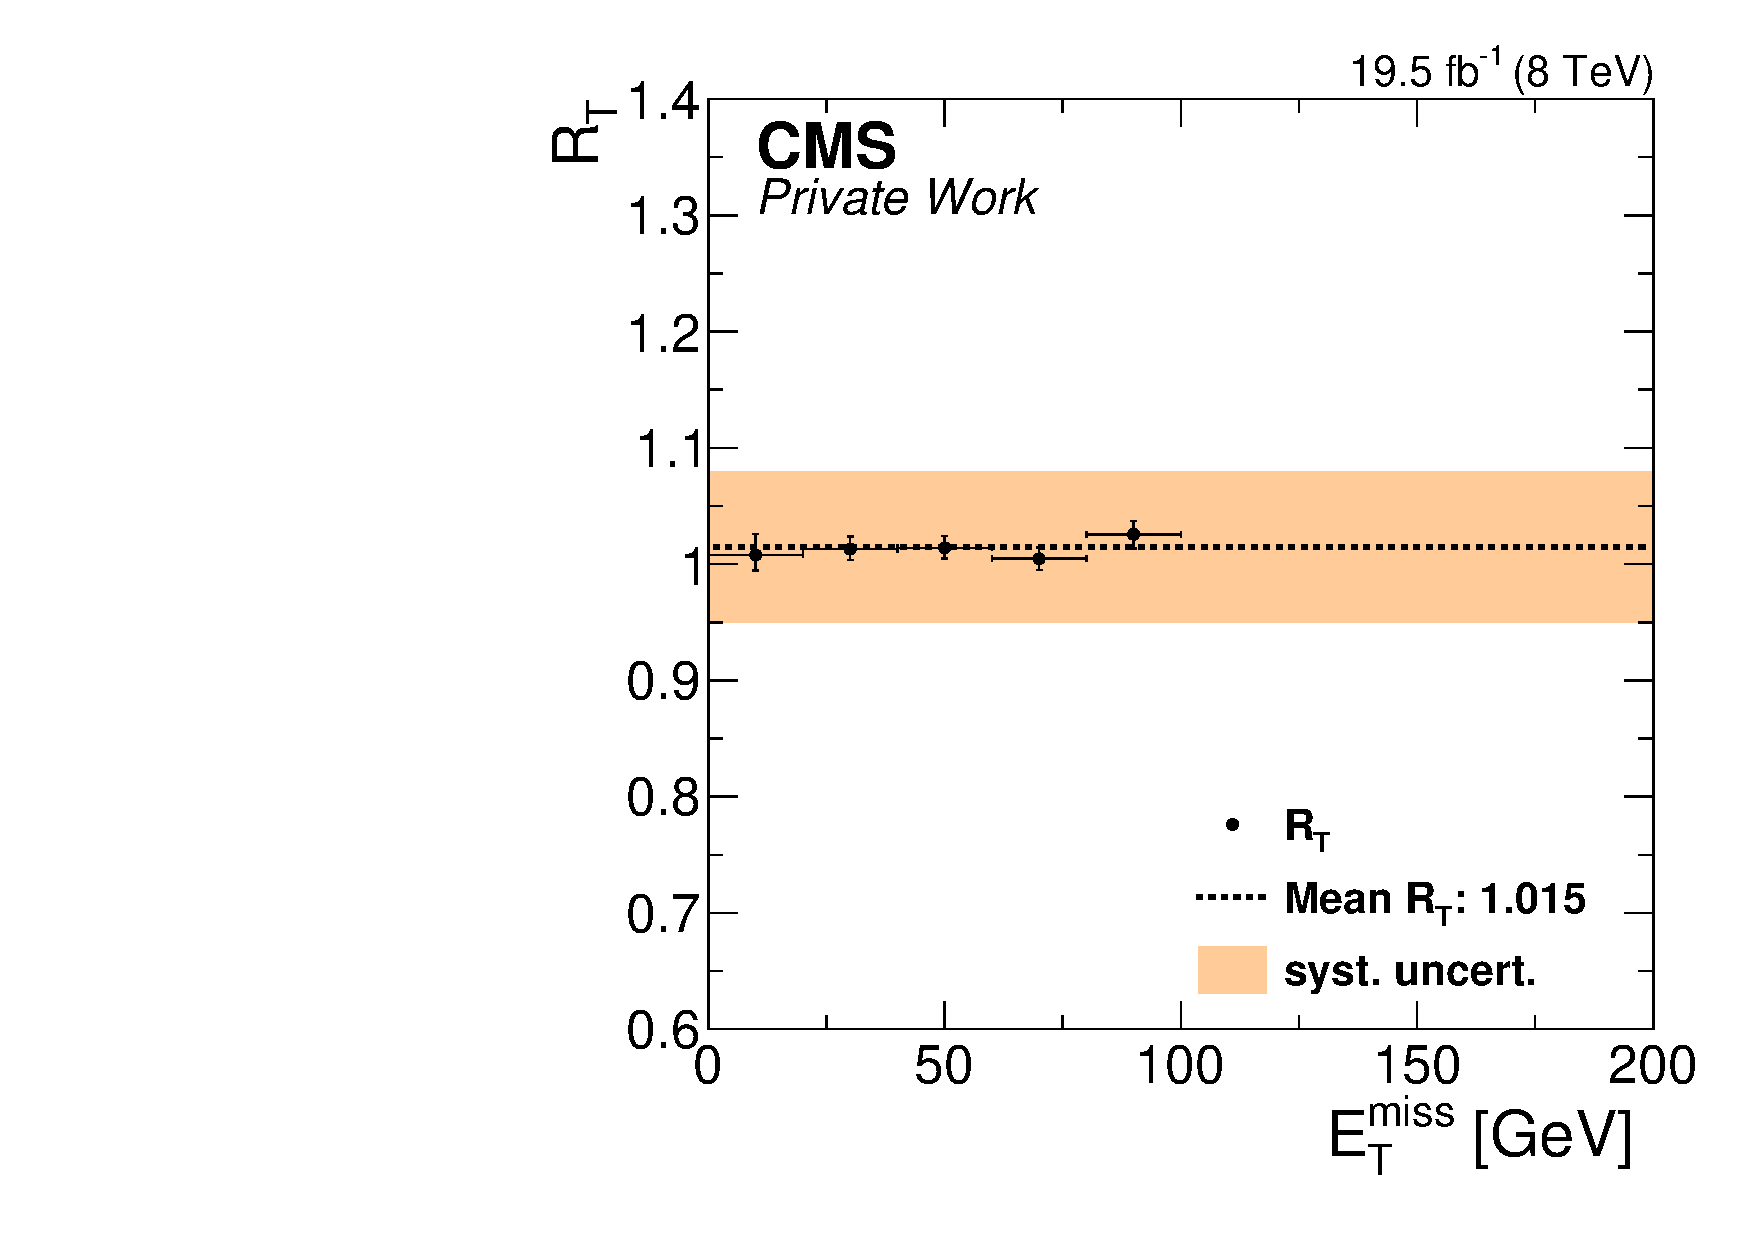
\includegraphics[width=\textwidth]{plots/BG/trigger/Triggereff_SFvsOF_Syst_AlphaT_HighHTExclusiveCentral_Full2012_MET_None.pdf}
\end{minipage}
\begin{minipage}[t]{0.49\textwidth}
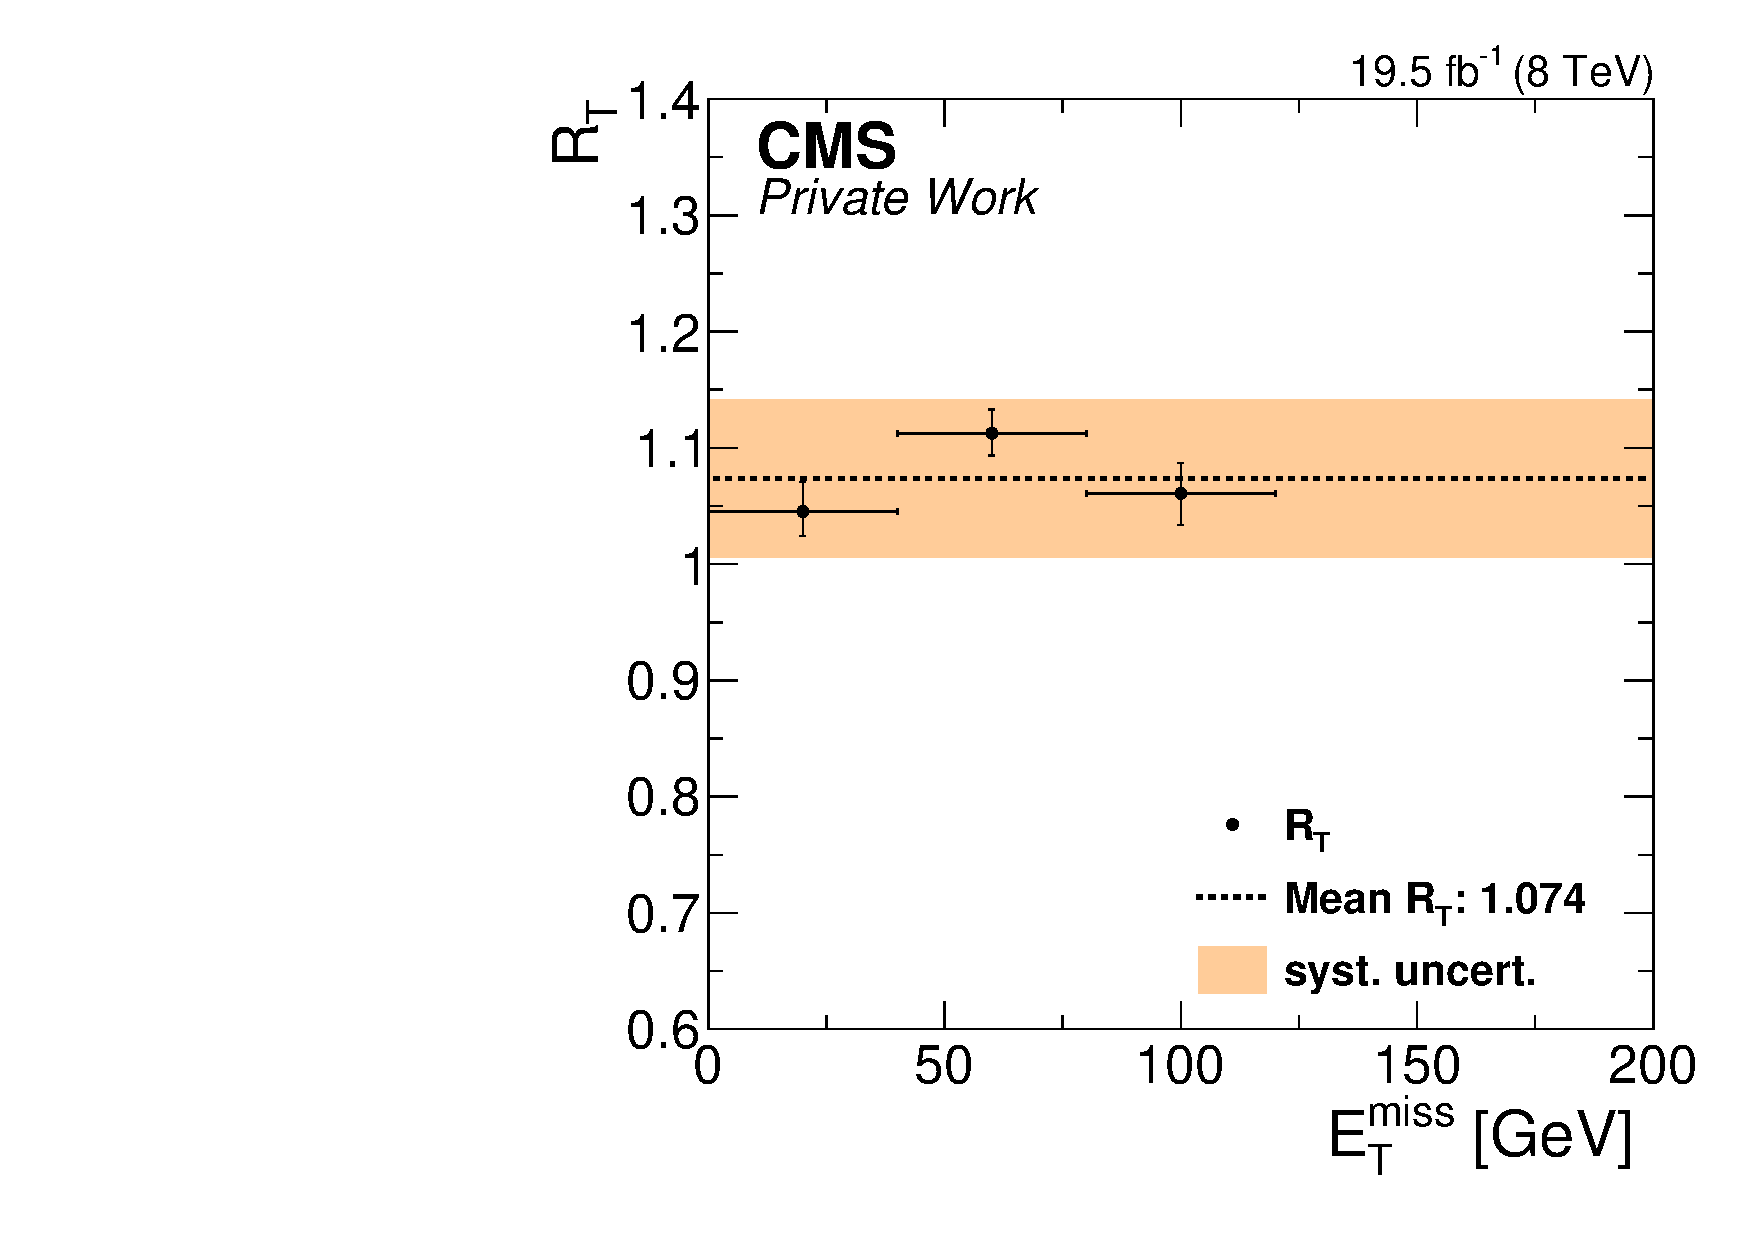
\includegraphics[width=\textwidth]{plots/BG/trigger/Triggereff_SFvsOF_Syst_AlphaT_HighHTExclusiveForward_Full2012_MET_None.pdf}
\end{minipage}
\begin{minipage}[t]{0.49\textwidth}
  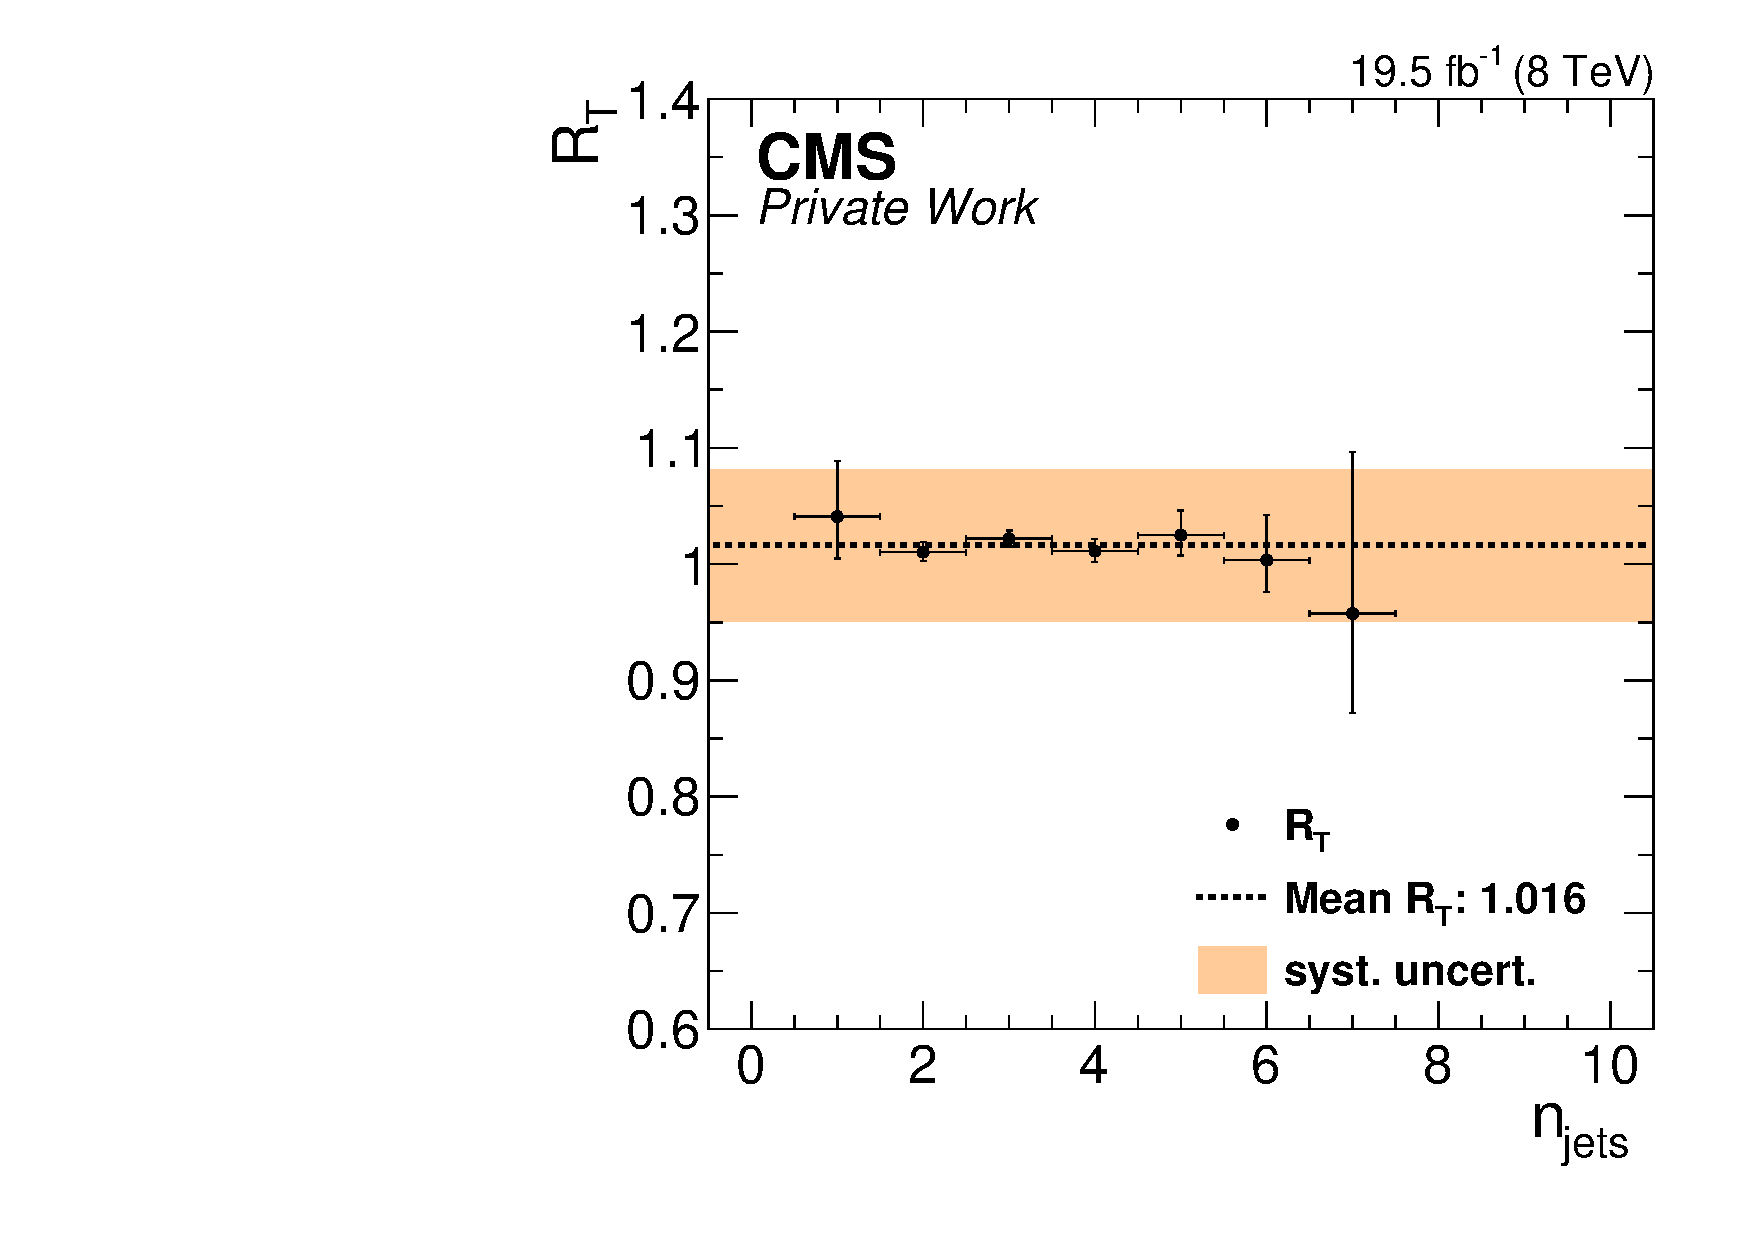
\includegraphics[width=\textwidth]{plots/BG/trigger/Triggereff_SFvsOF_Syst_AlphaT_HighHTExclusiveCentral_Full2012_NJets_None.pdf}
\end{minipage}
\begin{minipage}[t]{0.49\textwidth}
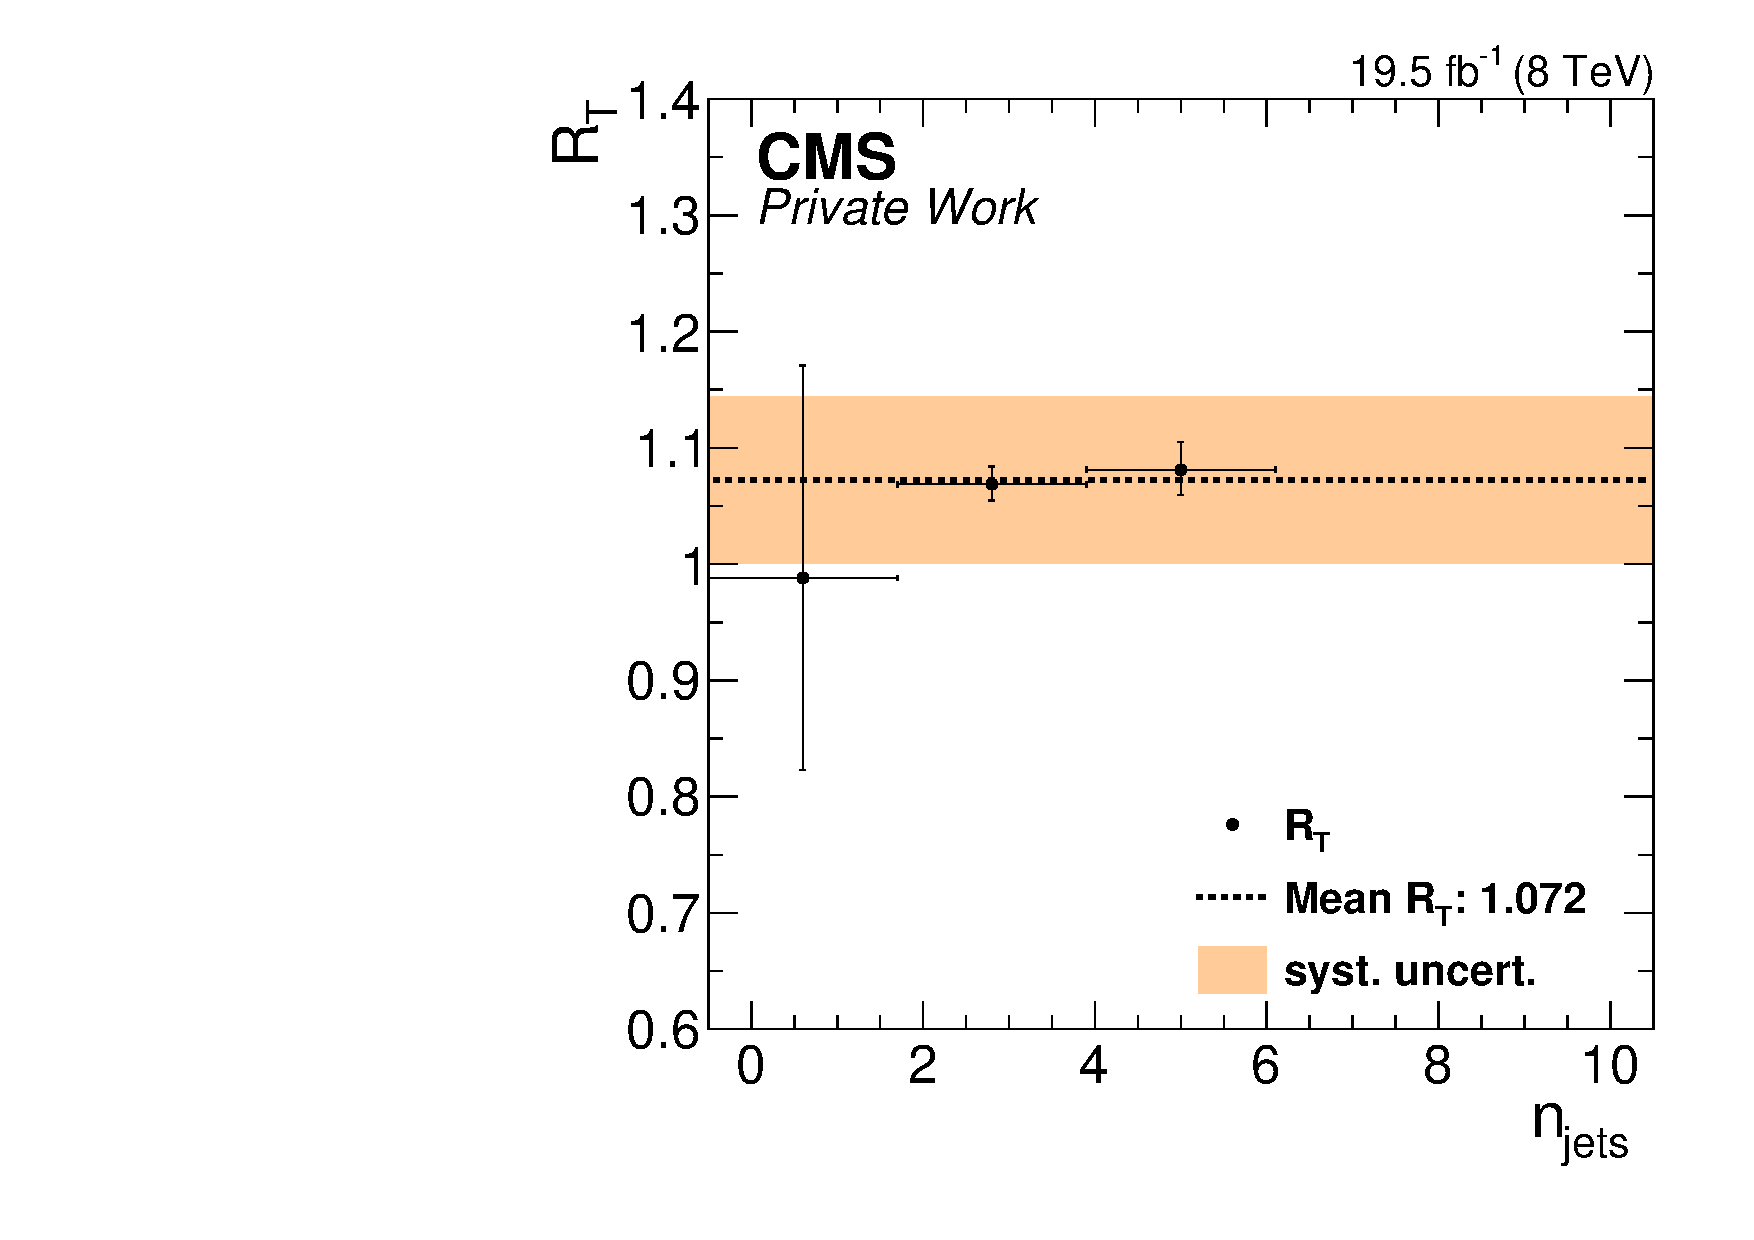
\includegraphics[width=\textwidth]{plots/BG/trigger/Triggereff_SFvsOF_Syst_AlphaT_HighHTExclusiveForward_Full2012_NJets_None.pdf}
\end{minipage}
\caption{Dependencies of $R_T$ on \mll (top), \MET (middle), and $N_{jets}$ (bottom) for the central (left) and forward (right) lepton selection. The results on data are shown in black. The central value is shown as a black dashed line while the systematic uncertainty is shown as an orange band.}
\label{fig:RTDependencies}
\end{figure} 
\subsubsection{Results of the factorization method}
The results of the factorization methods are summarized in Table~\ref{tab:factorization}. The factor $R_T$ is calculated from the trigger efficiencies in Table~\ref{tab:EffValues_Seperated} as $R_T = \sqrt{\frac{\epsilon_{ee}^{T}\cdot\epsilon_{\mu\mu}^{T} }{\epsilon_{e\mu}^{T}}}$. The resulting correction factors \Rsfof, \Reeof, and \Rmmof are calculated as described in equations~\ref{eq:nee}-\ref{eq:nsf}.  

\begin{table}[hbtp]
 \renewcommand{\arraystretch}{1.3}
 \setlength{\belowcaptionskip}{6pt}
 \centering
 \caption{Result of the determination of \Rsfof, \Reeof, and \Rmmof using the factorisation method.}
  \label{tab:factorisation}
  \begin{tabular}{l| c c| c c }

    & \multicolumn{2}{c}{Central} & \multicolumn{2}{c}{Forward} \\ 
    								
    \hline
    & Data & MC & Data & MC \\ 
 
    \hline
        \rmue       &  1.088$\pm$0.109  &  1.103$\pm$0.110      &  1.183$\pm$0.237 &   1.207$\pm$0.241    \\
        $R_{T}$       &  1.026$\pm$0.066  &  1.017$\pm$0.065      &  1.084$\pm$0.079 &   1.018$\pm$0.069    \\

\hline
\hline
        \Rsfof       &  1.029$\pm$0.067  &  1.031$\pm$0.067      &  1.099$\pm$0.088 &   1.103$\pm$0.091    \\
        \Reeof       &  0.471$\pm$0.116  &  0.465$\pm$0.117      &  0.458$\pm$0.259 &   0.449$\pm$0.264    \\
        \Rmmof       &  0.558$\pm$0.117  &  0.565$\pm$0.119      &  0.641$\pm$0.261 &   0.654$\pm$0.266    \\

  \end{tabular}
\end{table}



As for the direct measurements in the control region, the observed deviations of \Rsfof from one are small and inside the uncertainties of the method. Because the uncertainty on \rmue cancels out to a large degree in the calculation \Rsfof, the total uncertainty is dominated by the uncertainty on $R_T$, while for \Reeof and \Rmmof the uncertainty of \rmue is the dominant one. This results in much larger uncertainties on the latter two factors. The dependency of \Rsfof on \rmue and $R_T$ is illustrated in Figure~\ref{fig:rmuePropaganda}. The measured values of \rmue and \Rsfof are shown as straight lines, surrounded by bands indicating their uncertainties. The red line shows the value of \Rsfof corresponding to a given \rmue, under the assumption that the trigger efficiencies stay constant. The dashed black lines show the impact that the uncertainties on the trigger efficiencies have on the resulting \Rsfof. It can be seen that variations of \rmue inside its systematic uncertainties have only little effect on \Rsfof, while changes in the trigger efficiencies have a much larger impact. 


\begin{figure}[htbp]
\centering
\begin{minipage}[t]{0.49\textwidth}
  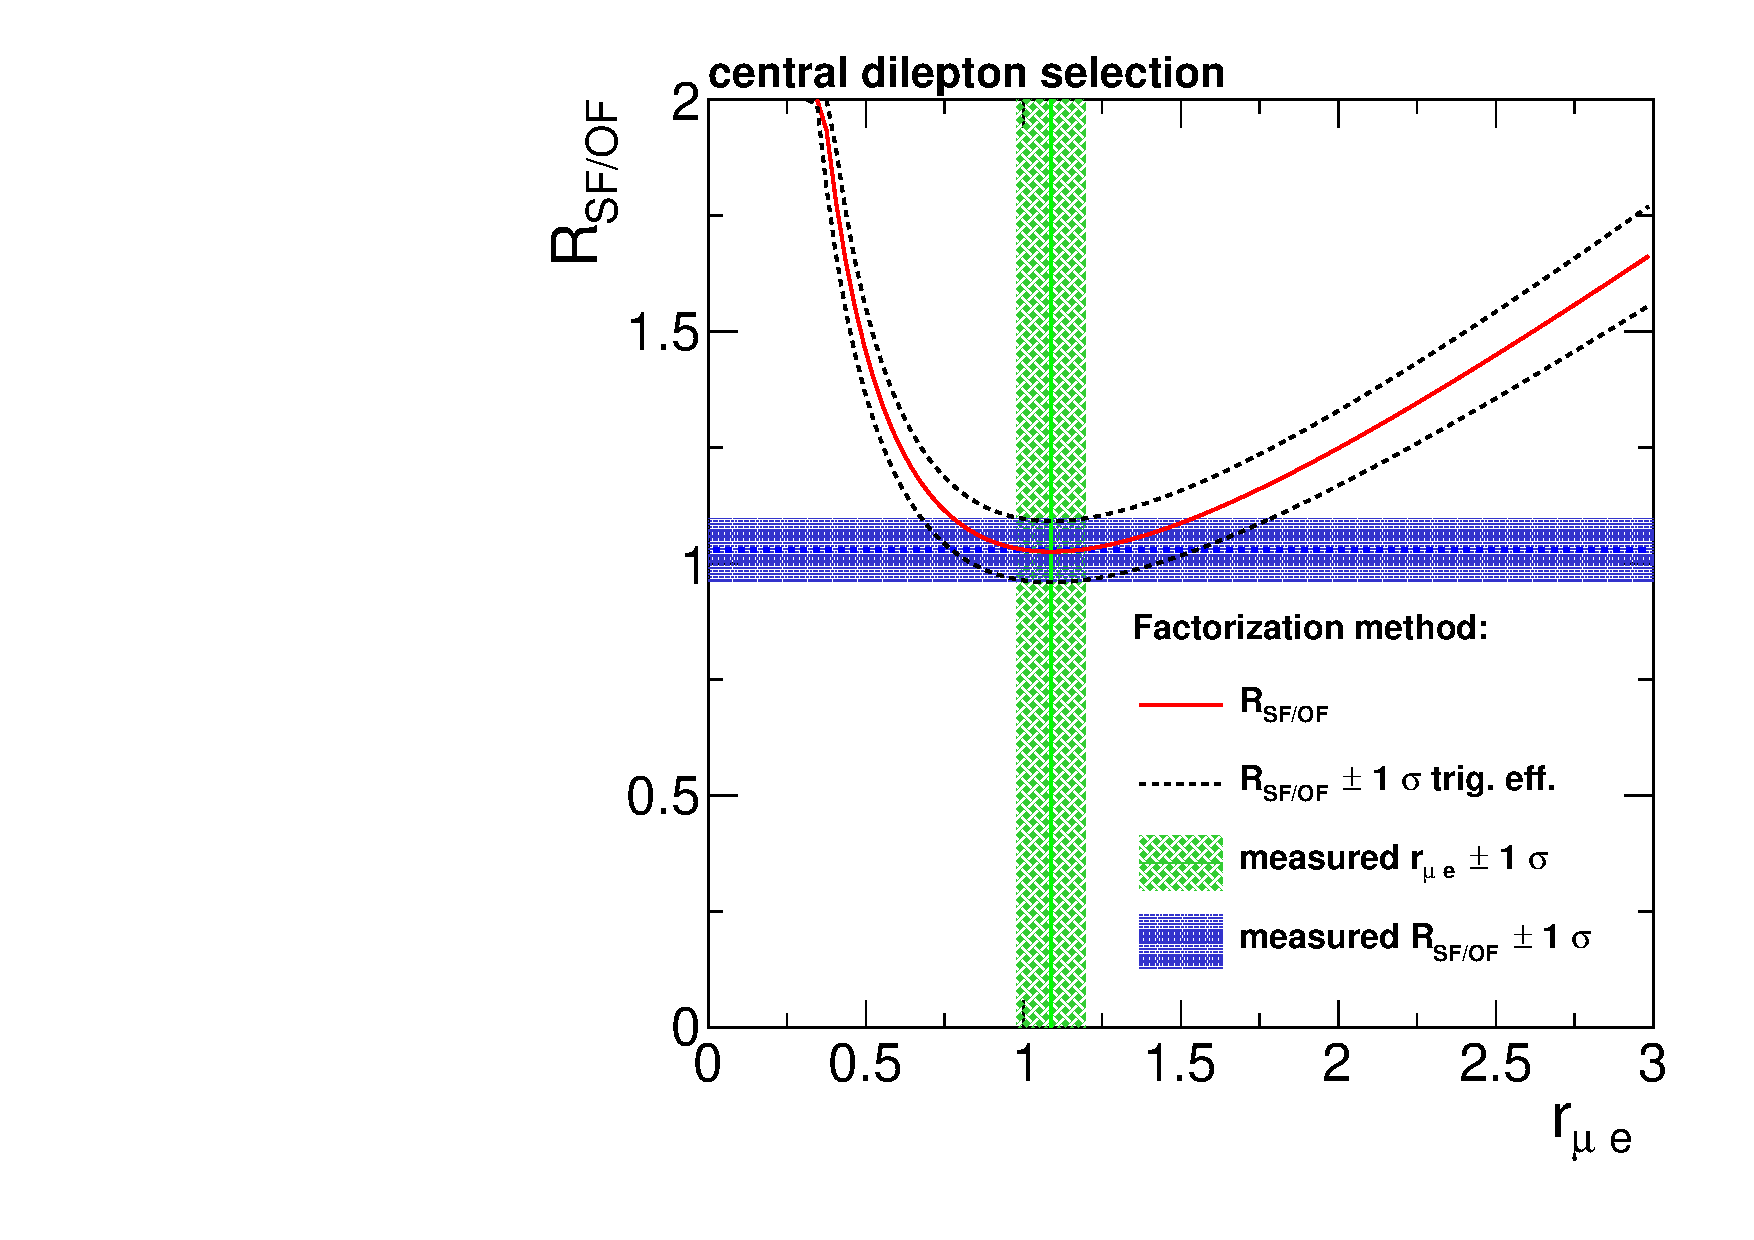
\includegraphics[width=\textwidth]{plots/BG/rmue/rMuEPropaganda_central.pdf}
\end{minipage}
\begin{minipage}[t]{0.49\textwidth}
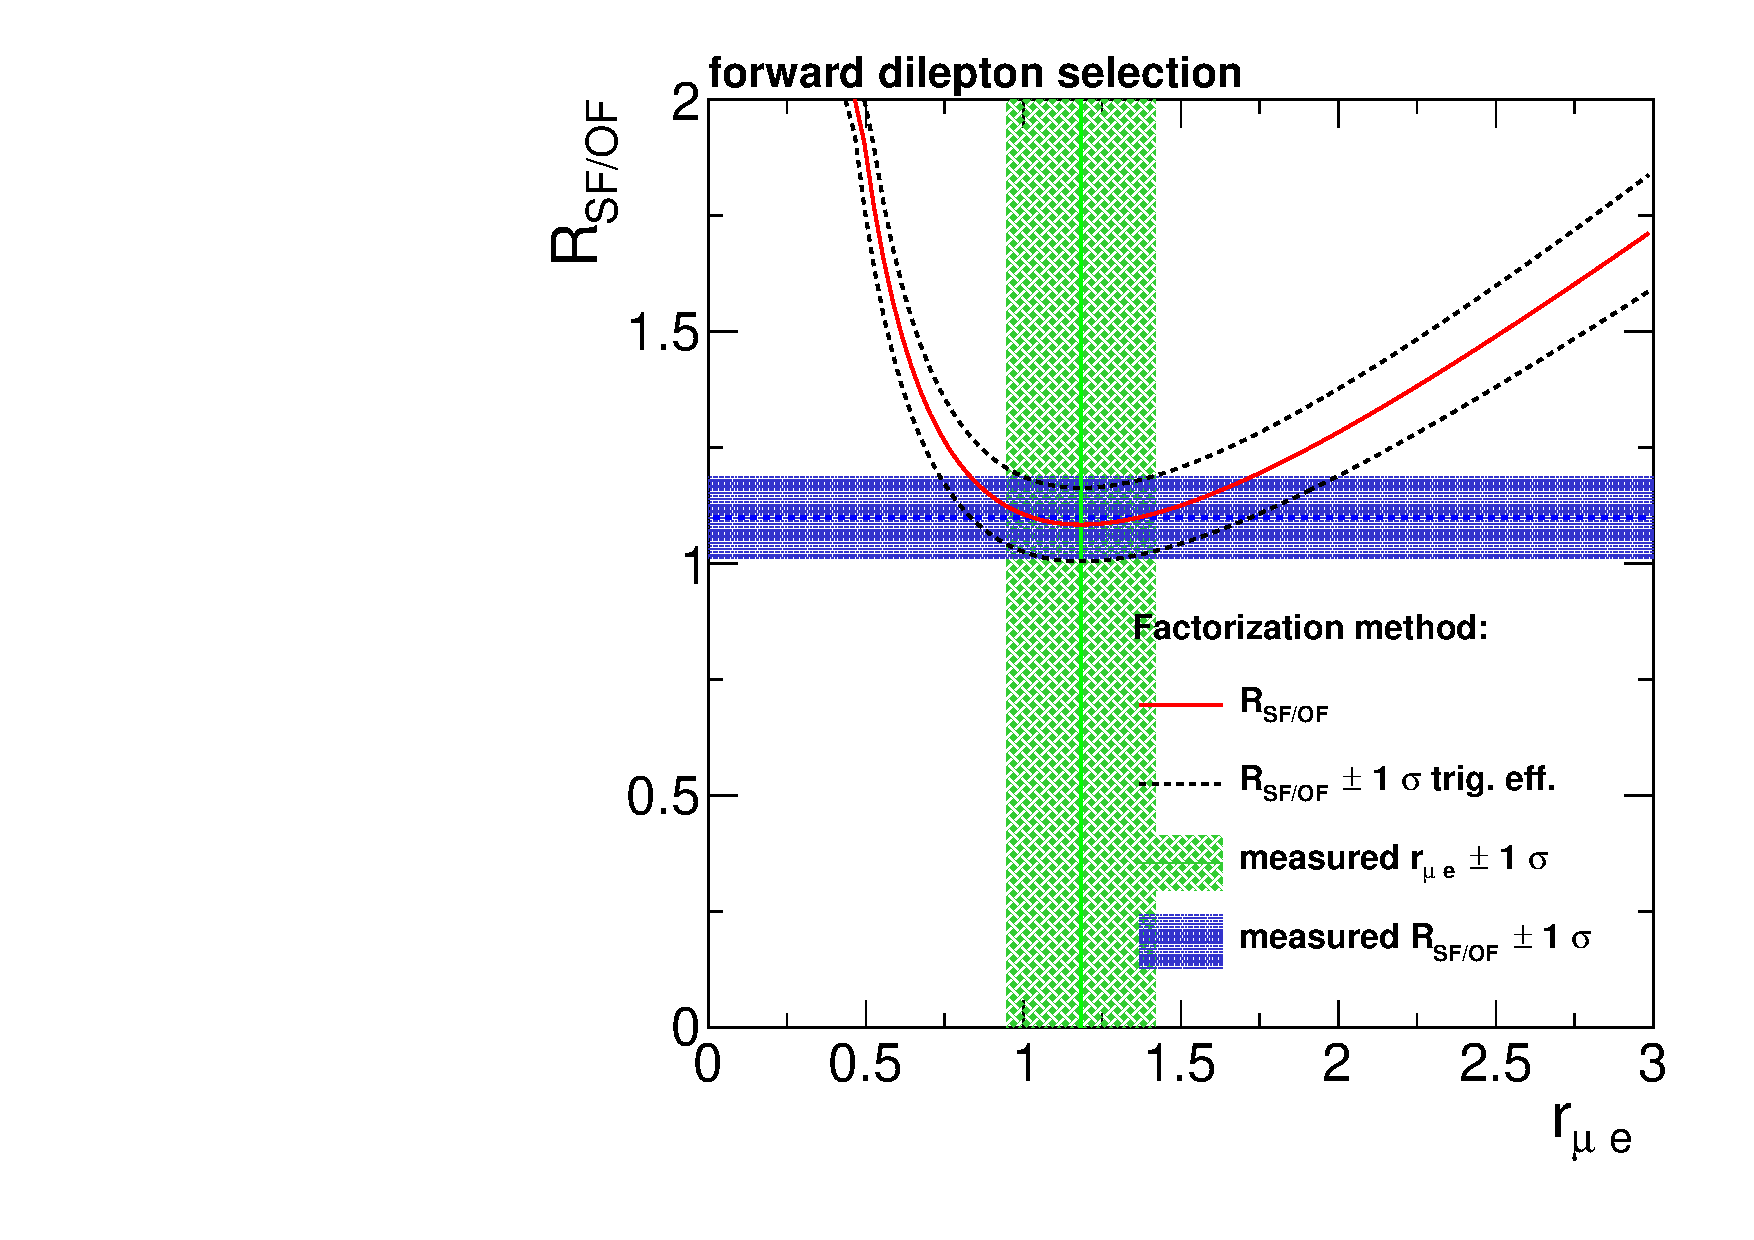
\includegraphics[width=\textwidth]{plots/BG/rmue/rMuEPropaganda_forward.pdf}
\end{minipage}

\caption{Dependency of \Rsfof on \rmue in the factorization method. The measured central values of \Rsfof and \rmue and their uncertainty are shown as the blue and green lines and bands. The red line illustrates the value of \Rsfof for a given \rmue if $R_T$ is kept constant. The impact of a variation of $R_T$ within its uncertainties on \Rsfof is shown by the dashed black lines.}
\label{fig:rmuePropaganda}
\end{figure} 

\subsection{Combined correction factors and resulting background estimates}
An overview of the resulting corrections factors of the measurement in the control region and the factorization method are shown in Table~\ref{tab:combinedRSFOF}. In all cases the results of the two methods agree very well within their uncertainties. Given the fact that they are performed on exclusive datasets and under the assumption that their uncertainties follow a Gaussian distribution, which is justified by the fact that they are either statistical in nature or assigned to cover statistical fluctuations in the dependency studies of \rmue and $R_T$, they can be combined using a weighted average. 

\begin{table}[hbtp]
 \renewcommand{\arraystretch}{1.3}
 \setlength{\belowcaptionskip}{6pt}
 \scriptsize
 \centering
 \caption{
     }
  \label{tab:combinedRSFOF}
  \begin{tabular}{l| c c| c c }
    & \multicolumn{4}{c}{\Rsfof}  \\ 

    & \multicolumn{2}{c}{Central} & \multicolumn{2}{c}{Forward} \\ 
    								
    \hline
    & Data & MC & Data & MC \
    \hline
        from factorization method       &  1.029\pm0.067  &  1.023\pm0.065      &  1.099\pm0.088 &   1.037\pm0.077    \\
        from direct measurement       &  1.012\pm0.039  &  1.010\pm0.008      &  1.000\pm0.105 &   1.010\pm0.014    \\
        weighted avarage       &  1.016\pm0.034  &  1.010\pm0.008      &  1.034\pm0.052 &   1.011\pm0.014    \\

\hline
    & \multicolumn{4}{c}{\Reeof}  \\ 

    & \multicolumn{2}{c}{Central} & \multicolumn{2}{c}{Forward} \\ 
    								
    \hline
    & Data & MC & Data & MC \
    \hline
        from factorization method       &  0.471\pm0.116  &  0.460\pm0.116      &  0.458\pm0.259 &   0.421\pm0.248    \\
        from direct measurement       &  0.459\pm0.026  &  0.457\pm0.005      &  0.439\pm0.093 &   0.427\pm0.008    \\
        weighted avarage       &  0.459\pm0.023  &  0.457\pm0.005      &  0.439\pm0.038 &   0.427\pm0.008    \\

\hline
    & \multicolumn{4}{c}{\Rmmof}  \\ 

    & \multicolumn{2}{c}{Central} & \multicolumn{2}{c}{Forward} \\ 
    								
    \hline
    & Data & MC & Data & MC \
    \hline
        from factorization method       &  0.558\pm0.117  &  0.563\pm0.118      &  0.641\pm0.261 &   0.617\pm0.250    \\
        from direct measurement       &  0.553\pm0.028  &  0.553\pm0.005      &  0.561\pm0.095 &   0.582\pm0.009    \\
        weighted avarage       &  0.553\pm0.026  &  0.553\pm0.005      &  0.563\pm0.043 &   0.582\pm0.009    \\

\hline
  \end{tabular}
\end{table}


 
A precision of about 4\% and 6\% on the translation from opposite flavour to same flavour is reached in the central and forward dilepton selection, respectively. Separating the lepton flavours, the uncertainty in \Reeof and \Rmmof is about 6\% for central and 9-10\% for forward leptons. This increase is caused by the missing cancellation of the uncertainty on \rmue and the increased statistical uncertainty in the direct measurement in the control region. Given that the weighted average is calculated separately for each flavour combination, \Reeof and \Rmmof do not add up exactly to \Rsfof, which in turn means that the sum of the background estimates for flavour-symmetric backgrounds in the \EE and \MM channels does not equal that in the SF channel. The OF yields in the \mll bins of the counting experiment together with the resulting background estimates in the different dilepton channels are shown in Table~\ref{tab:FlavSymBackgrounds}. 

\begin{table}[hbtp]
 \renewcommand{\arraystretch}{1.3}
 \setlength{\belowcaptionskip}{6pt}
 \scriptsize
 \centering
 \caption{Resulting estimates for flavour-symmetric backgrounds. Given is the observed event yield in OF events and the resulting estimate after applying the correction, separately for the SF, \EE, and \MM channels. Statistical and systematic uncertainties are given separately.
     }
  \label{tab:FlavSymBackgrounds}
  \begin{tabular}{l| cc | cc | cc}
    							& \multicolumn{2}{c}{Low-mass} & \multicolumn{2}{c}{On-\Z} & \multicolumn{2}{c}{High-mass} \\ 

    \hline
                                &  Central        & Forward  &  Central  & Forward   &  Central        & Forward \\ 

    \hline
        Observed OF events       &  737                   & 138              &  364            &  131       &   779           &   393    \\

    \hline
        Estimate in SF channel    & $746\pm27\pm26$        & $144\pm12\pm7$  &  $368\pm19\pm13$ & $137\pm11\pm7$ & $789\pm28\pm28$ & $411\pm20\pm21$ \\

        Estimate in \EE channel    & $337\pm12\pm19$        & $61\pm5\pm6$  &  $166\pm8\pm9$ & $58\pm5\pm5$ & $357\pm12\pm21$ & $175\pm8\pm17$ \\

        Estimate in \MM channel    & $405\pm14\pm21$        & $79\pm6\pm6$  &  $200\pm10\pm10$ & $74\pm6\pm6$ & $428\pm15\pm23$ & $224\pm11\pm19$ \\


  \end{tabular}
\end{table}







\subsection{Validation of background estimates}
To judge the performance of the estimation methods for flavour-symmetric backgrounds, they are applied to simulation. In Table~\ref{tab:MCClosure} the resulting SF and OF yields after application of the signal selection are shown separately for the central and forward dilepton selection. The OF yields are corrected with the \Rsfof values derived for MC shown in Table~\ref{tab:combinedRSFOF}. For completely flavour-symmetric processes, such as \ttbar, Drell--Yan production decaying to $\tau\tau$ or single top-quark production, the difference between the SF and OF yields is compatible with zero within the statistical uncertainties of the simulation and the systematic uncertainties of the method. Other systematic uncertainties affecting the simulation are the same for SF and OF lepton pairs and are therefore not considered here. 

\begin{table}[hbtp]
 \renewcommand{\arraystretch}{1.3}
 \setlength{\belowcaptionskip}{6pt}
 \centering
 \caption{Event yields in the signal region in simulation for both SF lepton pairs and the prediction SF$^{\text{pred}}$, derived by multiplying the OF yield by \Rsfof. The uncertainty on SF$^{\text{pred}}$ includes the systematic uncertainty on \Rsfof. The event yields are compared separated into flavour-symmetric and Drell--Yan backgrounds. Processes contributing to both categories have been sorted into the Drell--Yan category.}
  \label{tab:MCClosure}
  \begin{tabular}{l| ccc | ccc }
    							& \multicolumn{3}{c|}{Central} & \multicolumn{3}{c}{Forward} \\ 

    \hline
								&  SF        & SF$^{\text{pred}}$  &  SF-SF$^{\text{pred}}$  & SF   &  SF$^{\text{pred}}$        & SF-SF$^{\text{pred}}$ \\ 

    \hline
\ttbar & 2214$\pm$9 & 2200$\pm$32 & 14$\pm$33 & 689$\pm$5 & 684$\pm$16 & 5$\pm$17 \\
$\Z/\gamma^{*}\rightarrow \ell\ell$ (\EE,\MM) & 49$\pm$11 & 0$\pm$0 & 49$\pm$11 & 24$\pm$8 & 4$\pm$4 & 20$\pm$9 \\
$\Z/\gamma^{*}\rightarrow \ell\ell$ $(\tau \tau)$ & 72$\pm$13 & 59$\pm$12 & 13$\pm$18 & 14$\pm$6 & 17$\pm$6 & -3$\pm$9 \\
Single t & 144$\pm$8 & 137$\pm$8 & 6$\pm$12 & 38$\pm$4 & 43$\pm$4 & -6$\pm$6 \\
WW, \Z{}\Z, W\Z & 121$\pm$2 & 77$\pm$2 & 45$\pm$3 & 51$\pm$1 & 34$\pm$2 & 17$\pm$2 \\
Other SM & 89$\pm$6 & 81$\pm$6 & 9$\pm$8 & 30$\pm$4 & 22$\pm$3 & 8$\pm$5 \\
\hline
Flav. sym. backgrounds & 2559$\pm$19 & 2531$\pm$41 & 28$\pm$45 & 795$\pm$10 & 793$\pm$22 & 1$\pm$24 \\
Drell--Yan backgrounds & 130$\pm$11 & 21$\pm$1 & 109$\pm$11 & 51$\pm$8 & 11$\pm$4 & 40$\pm$9 \\
Total simulation & 2689$\pm$22 & 2553$\pm$40 & 136$\pm$46 & 846$\pm$13 & 804$\pm$21 & 42$\pm$25 \\


  \end{tabular}
\end{table}



 As expected, deviations from flavour-symmetry are observed only for processes containing a \Z boson, most notable Drell--Yan production decaying to light leptons, but also WZ or ZZ production and more rare processes like $t\bar{t}$Z production. It can therefore be concluded that the background prediction for flavour-symmetric processes performs well within the uncertainties of the methods presented above. The validity of this cross check is restricted to processes well modelled in simulation. As the modelling of non-prompt leptons is in general less reliable, more detailed studies are performed on data to ensure that flavour-symmetry also holds for the small contribution of non-prompt leptons to the final event selection.
\subsubsection*{Study of non-prompt leptons}
As a preface to studies performed on data, the contribution of non-prompt leptons is examined using MC truth information. A data driven estimate for this contribution is derived from leptons with relaxed isolation criteria.
\paragraph*{Non-prompt leptons in simulation}
The origin of the leptons in the events contribution to the signal selection is studied in simulation by matching the reconstructed lepton to the generated particles with the smallest spatial separation $\Delta R$. The difference in generated and reconstructed \pt must not exceed twice the generated \pt. The parentage of the matched generated particle is used to determine of the lepton originates from a prompt decay, a heavy flavour decay inside a jet, or a jet that was misreconstructed as a lepton. The contribution of non-prompt leptons to the signal selection is studied in \ttbar events, where the two b-jets are a source for leptons from heavy flavour decays. 

All events where at least one of the leptons is not matched to a generated electron or muon and/or does not originate directly or via and intermediate $\tau$ lepton from a W boson are considered non-prompt. The resulting \mll distributions are shown in Figure~\ref{fig:nonPromptMC} for an inclusive dilepton selection on the left and the combined central and forward signal selection on the right. Good agreement between SF and OF pairs can be seen, with a slight tendency towards OF. 
\begin{figure}[htbp]
\centering
\begin{minipage}[t]{0.49\textwidth}
  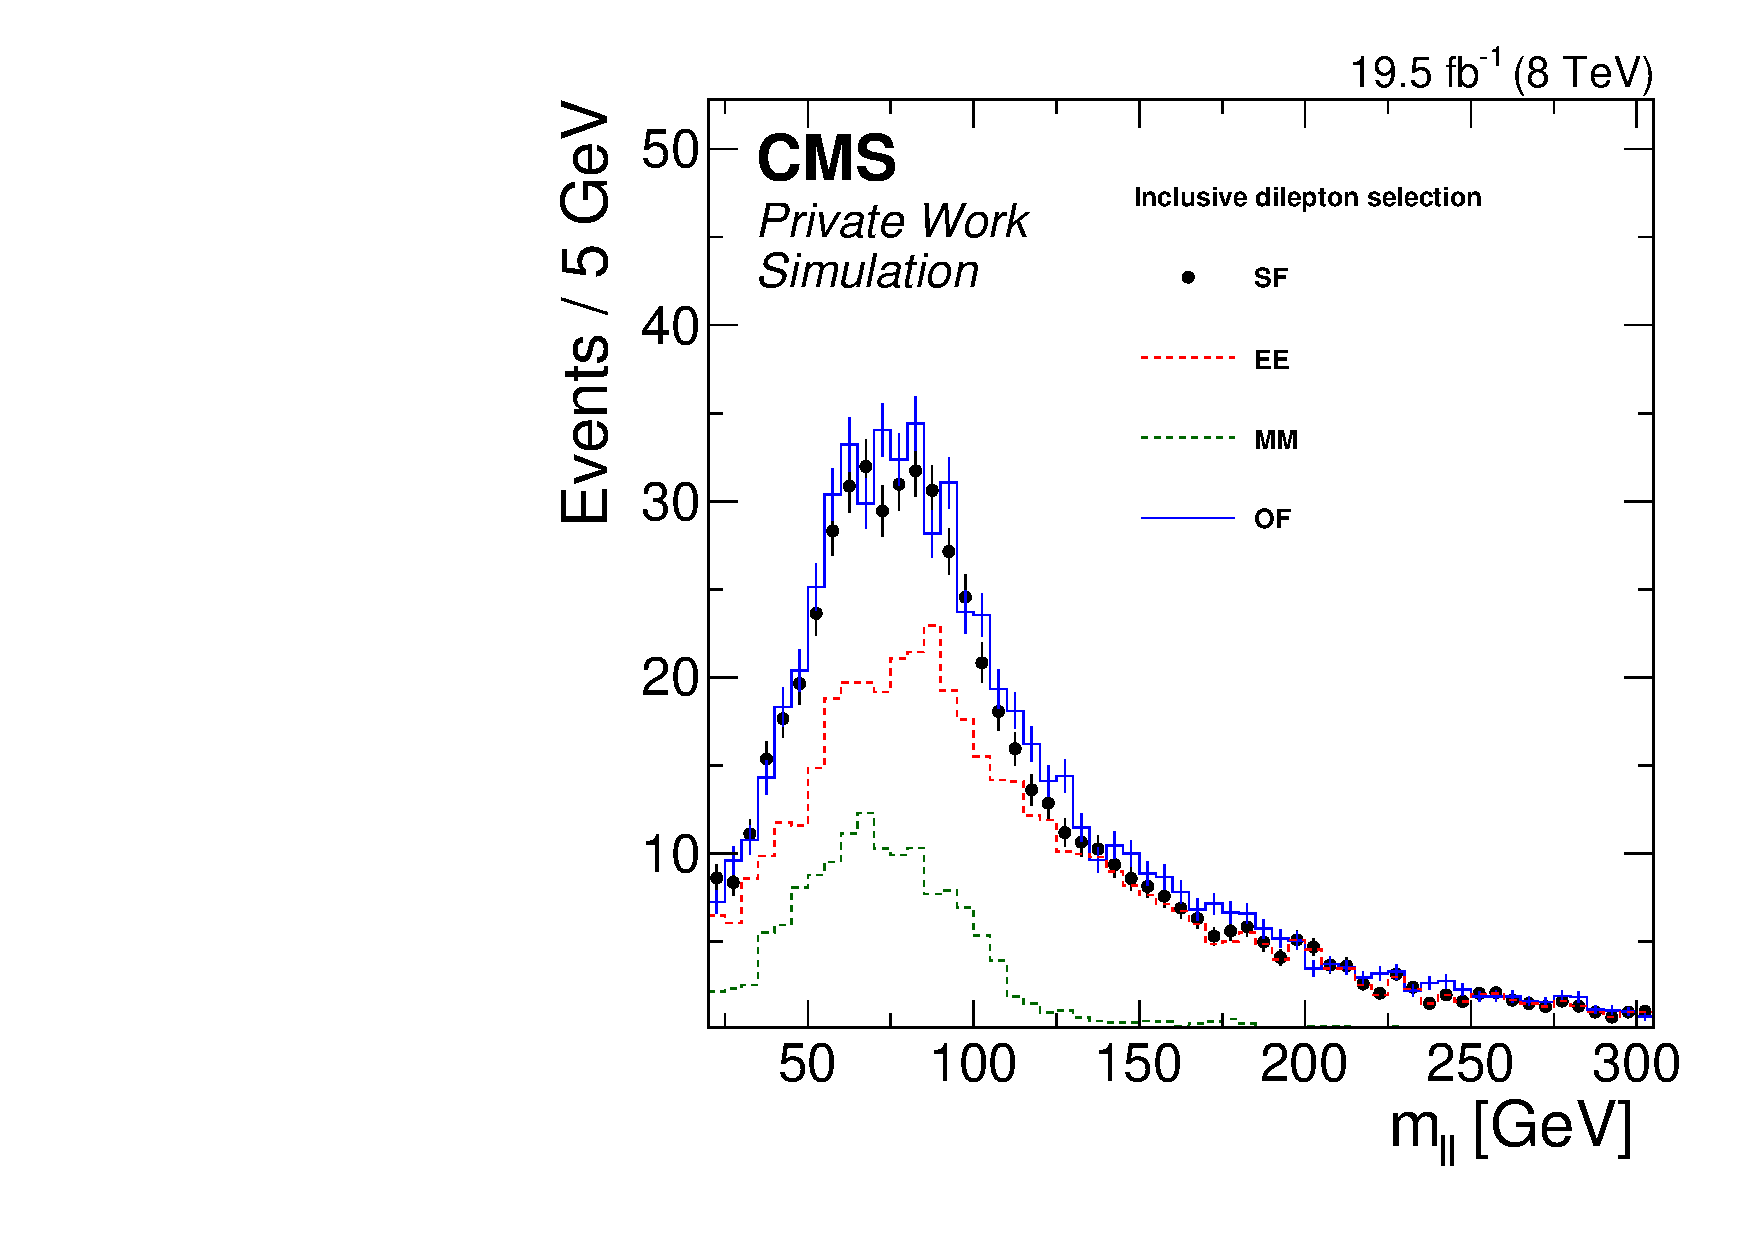
\includegraphics[width=\textwidth]{plots/BG/nonPrompt/nonPromptMC_Inclusive_Full2012_Mll_None.pdf}
\end{minipage}
\begin{minipage}[t]{0.49\textwidth}
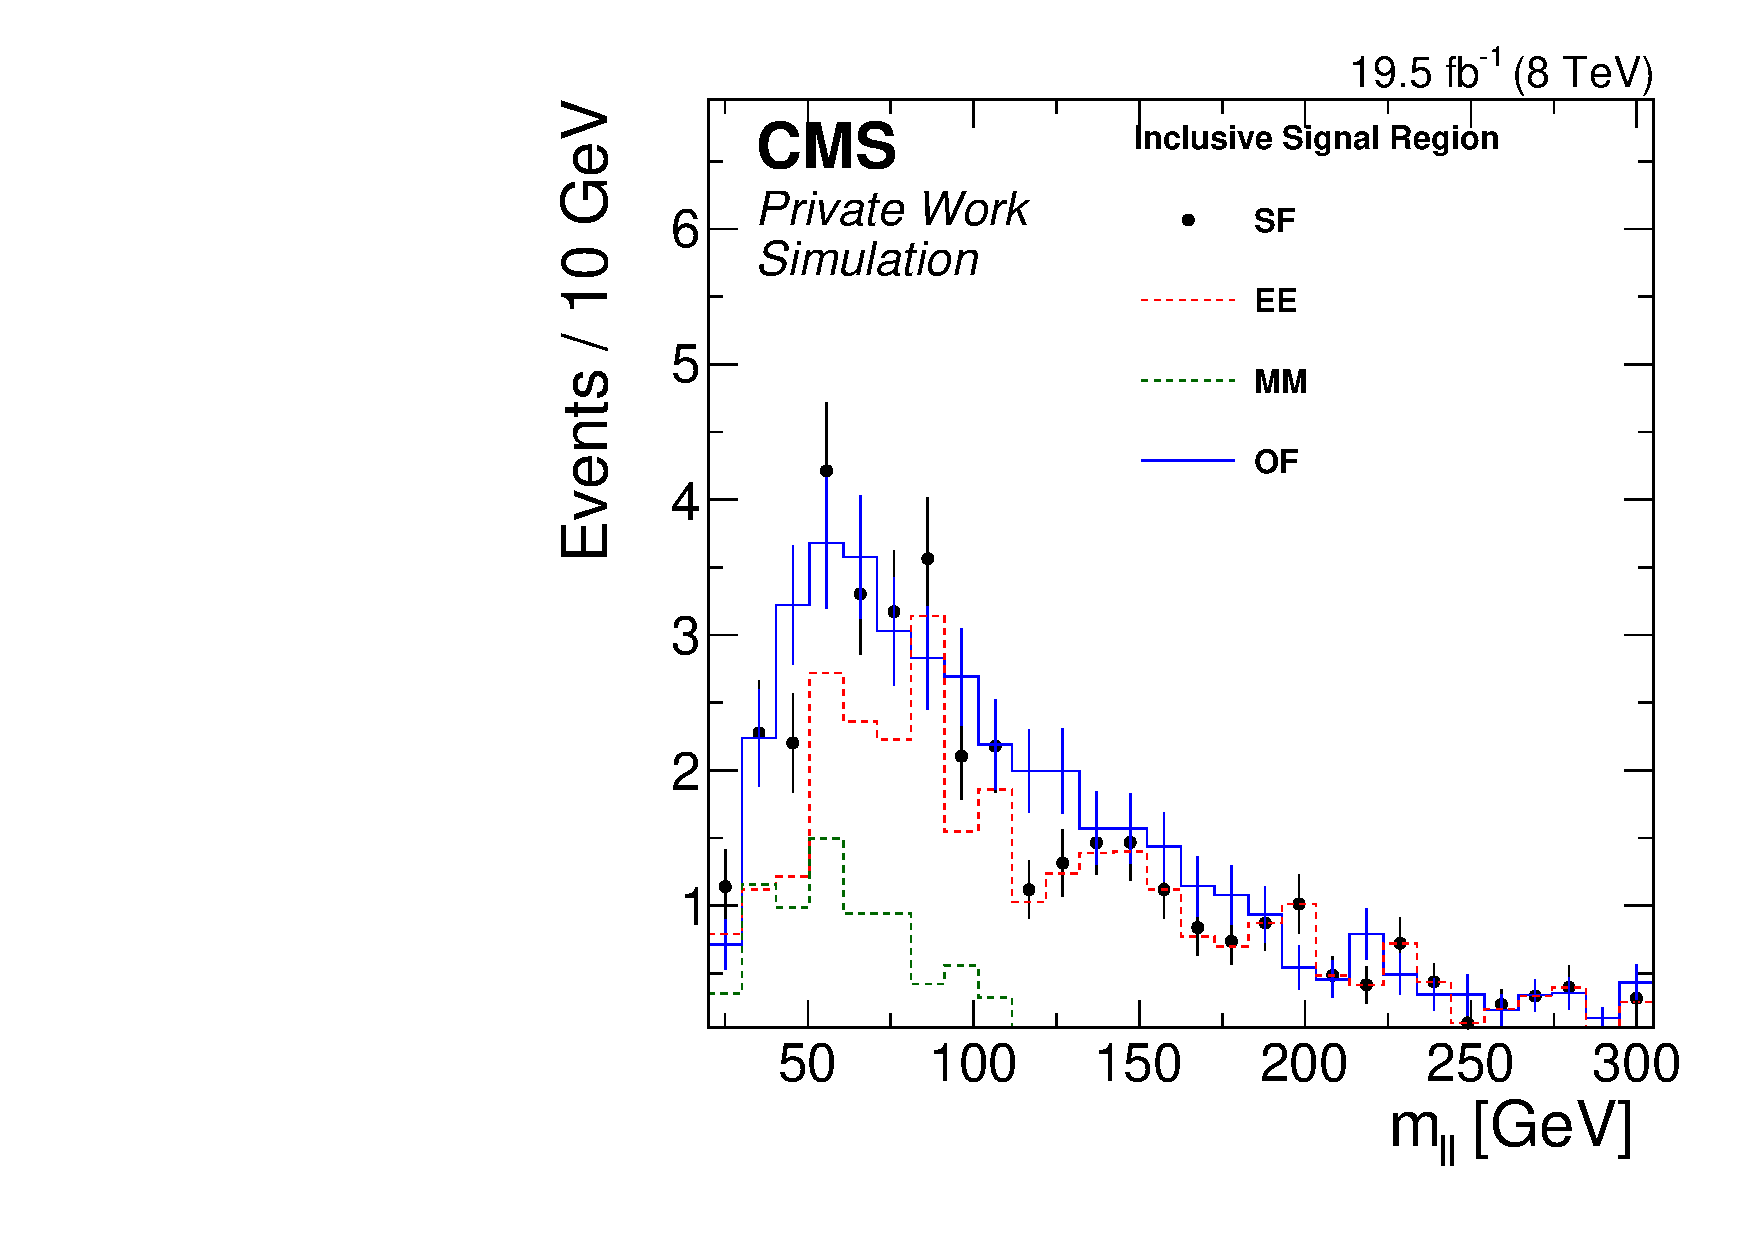
\includegraphics[width=\textwidth]{plots/BG/nonPrompt/nonPromptMC_SignalInclusive_Full2012_Mll_None.pdf}
\end{minipage}
\caption{Distribution of \mll for lepton pairs with at least one non-prompt lepton in simulation for an inclusive dilepton selection (left) and the signal selection (right). The contributions of \EE, \MM, and \EM pairs are shown as red, green, and blue lines, respectively. The combined SF pairs are shown as the black points.}
\label{fig:nonPromptMC}
\end{figure} 
The event yields are summarized in Table~\ref{tab:nonPromptTableMC}. It can be seen that the contribution of non-prompt electrons exceeds that of non-prompt muons. The event yields for SF and OF lepton pairs are very similar, with a slight preference to OF leptons. This indicates that this type of backgrounds is covered by the estimates for flavour-symmetric backgrounds, at least in simulation.

\begin{table}[!htbp]
 \renewcommand{\arraystretch}{1.2}
 \begin{center}
  \caption{Number of events with non-prompt leptons in an inclusive dilepton selection, and the central and forward signal regions for \ttbar simulation.}
  \begin{tabular}{l|ccccc}
   \hline
   \hline
                                    & \EE & \MM & SF & \EM    & \Rsfof        \\
   \hline
       Inclusive      &  456.0$\pm$5.2  & 140.3$\pm$3.3 & 596.2$\pm$8.4  & 637.5$\pm$6.3          &  0.94$\pm$0.02    \\
       Signal central      &  20.2$\pm$1.0  & 4.9$\pm$0.6 & 25.0$\pm$1.6  & 26.2$\pm$1.2          &  0.95$\pm$0.07    \\
       Signal forward      &  9.8$\pm$0.7  & 2.8$\pm$0.5 & 12.6$\pm$1.2  & 14.2$\pm$0.9          &  0.89$\pm$0.10    \\

 \end{tabular}
 \label{tab:nonPromptTableMC}
 \end{center}
\end{table}


\paragraph*{Estimate of non-prompt contributions with tight-to-loose ratios}
The contribution of non-prompt leptons to the signal selection can be estimated on data from control samples enriched in non-prompt leptons.\fixme{Reference origin of method. Can I cite ANs?} These samples are obtained by relaxing the isolation requirements on the leptons from requiring the relative isolation to be $<$ 0.15 to $<$ 1.0. The probability of a prompt or non-prompt lepton that passes this ``loose'' selection to also pass the default ``tight'' selection allows to calculate the different contributions of prompt-prompt, prompt-non-prompt and non-prompt-non-prompt dilepton events to the signal selection. 

The probability for a non-prompt loose lepton to pass also the tight selection, often referred to as ``fake rate'' $f$ is calculated in an event sample enriched in non-prompt leptons. It is collected by prescaled low-\pt single lepton trigger, see section \fixme{add this somewhere}. At least one jet with $\pt > \unit{50}{\giga\electronvolt}$ is required. To reject prompt leptons from \Wjets events, \MET and the transverse mass of the lepton-\MET system are both required to be $\unit{<20}{\giga\electronvolt}$. The resulting fake rates as a function of lepton \pt and $\eta$ are shown in Figure~\ref{fig:fakeRate}. For low \pt, the value for electrons is about 0.25 while for muons it is about 0.07. Dependencies on both \pt and $\eta$ are observed. The fake rate is therefore measured and applied as a function of both variables. The increase for higher \pt is however understood as arising from an increasing contamination from prompt leptons. Therefore for all leptons with $\unit{\pt > 40}{\giga\electronvolt}$, the values measured between $\unit{35}{\giga\electronvolt}$ and $\unit{40}{\electronvolt}$ are used.  
\begin{figure}[htbp]
\centering
\begin{minipage}[t]{0.49\textwidth}
  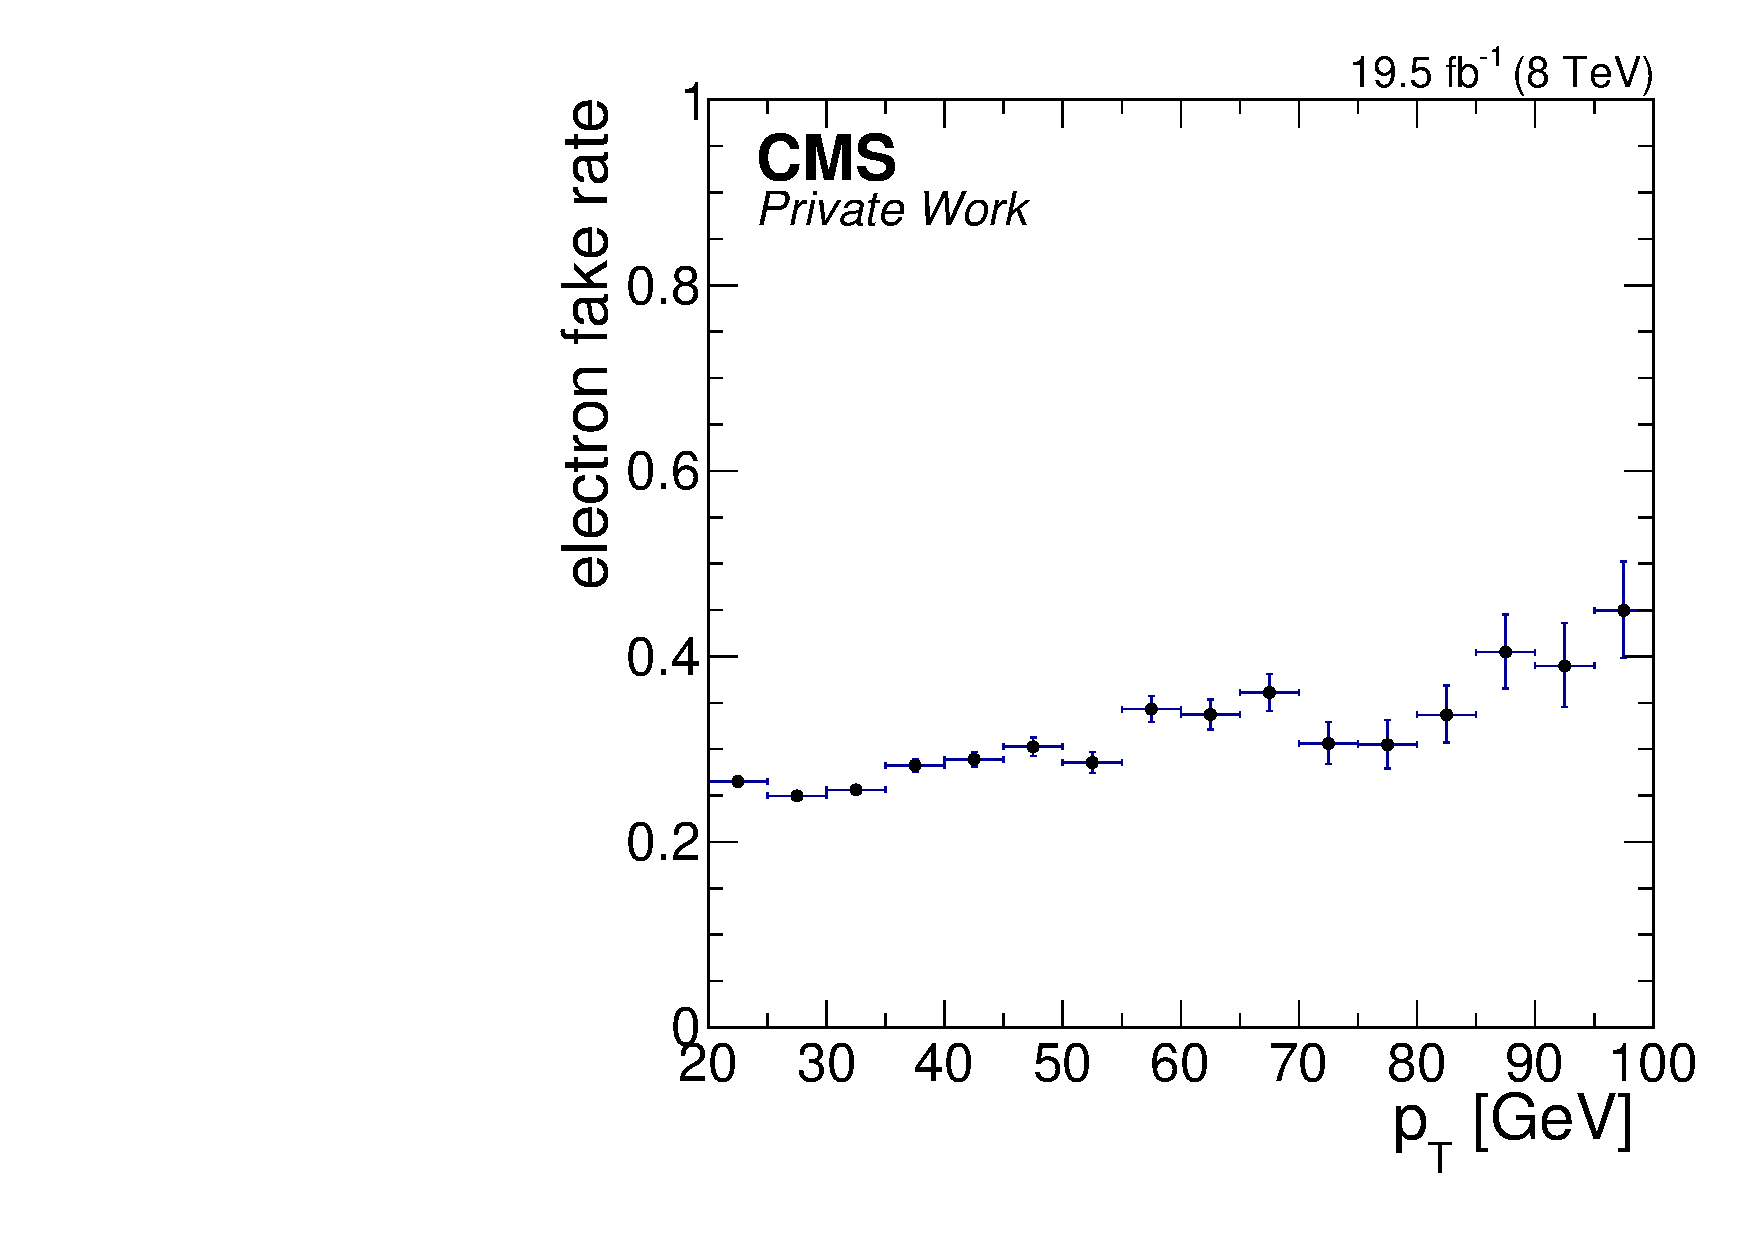
\includegraphics[width=\textwidth]{plots/BG/nonPrompt/fakeRate_ele_Inclusive_Full2012_TrailingPt_range100.pdf}
\end{minipage}
\begin{minipage}[t]{0.49\textwidth}
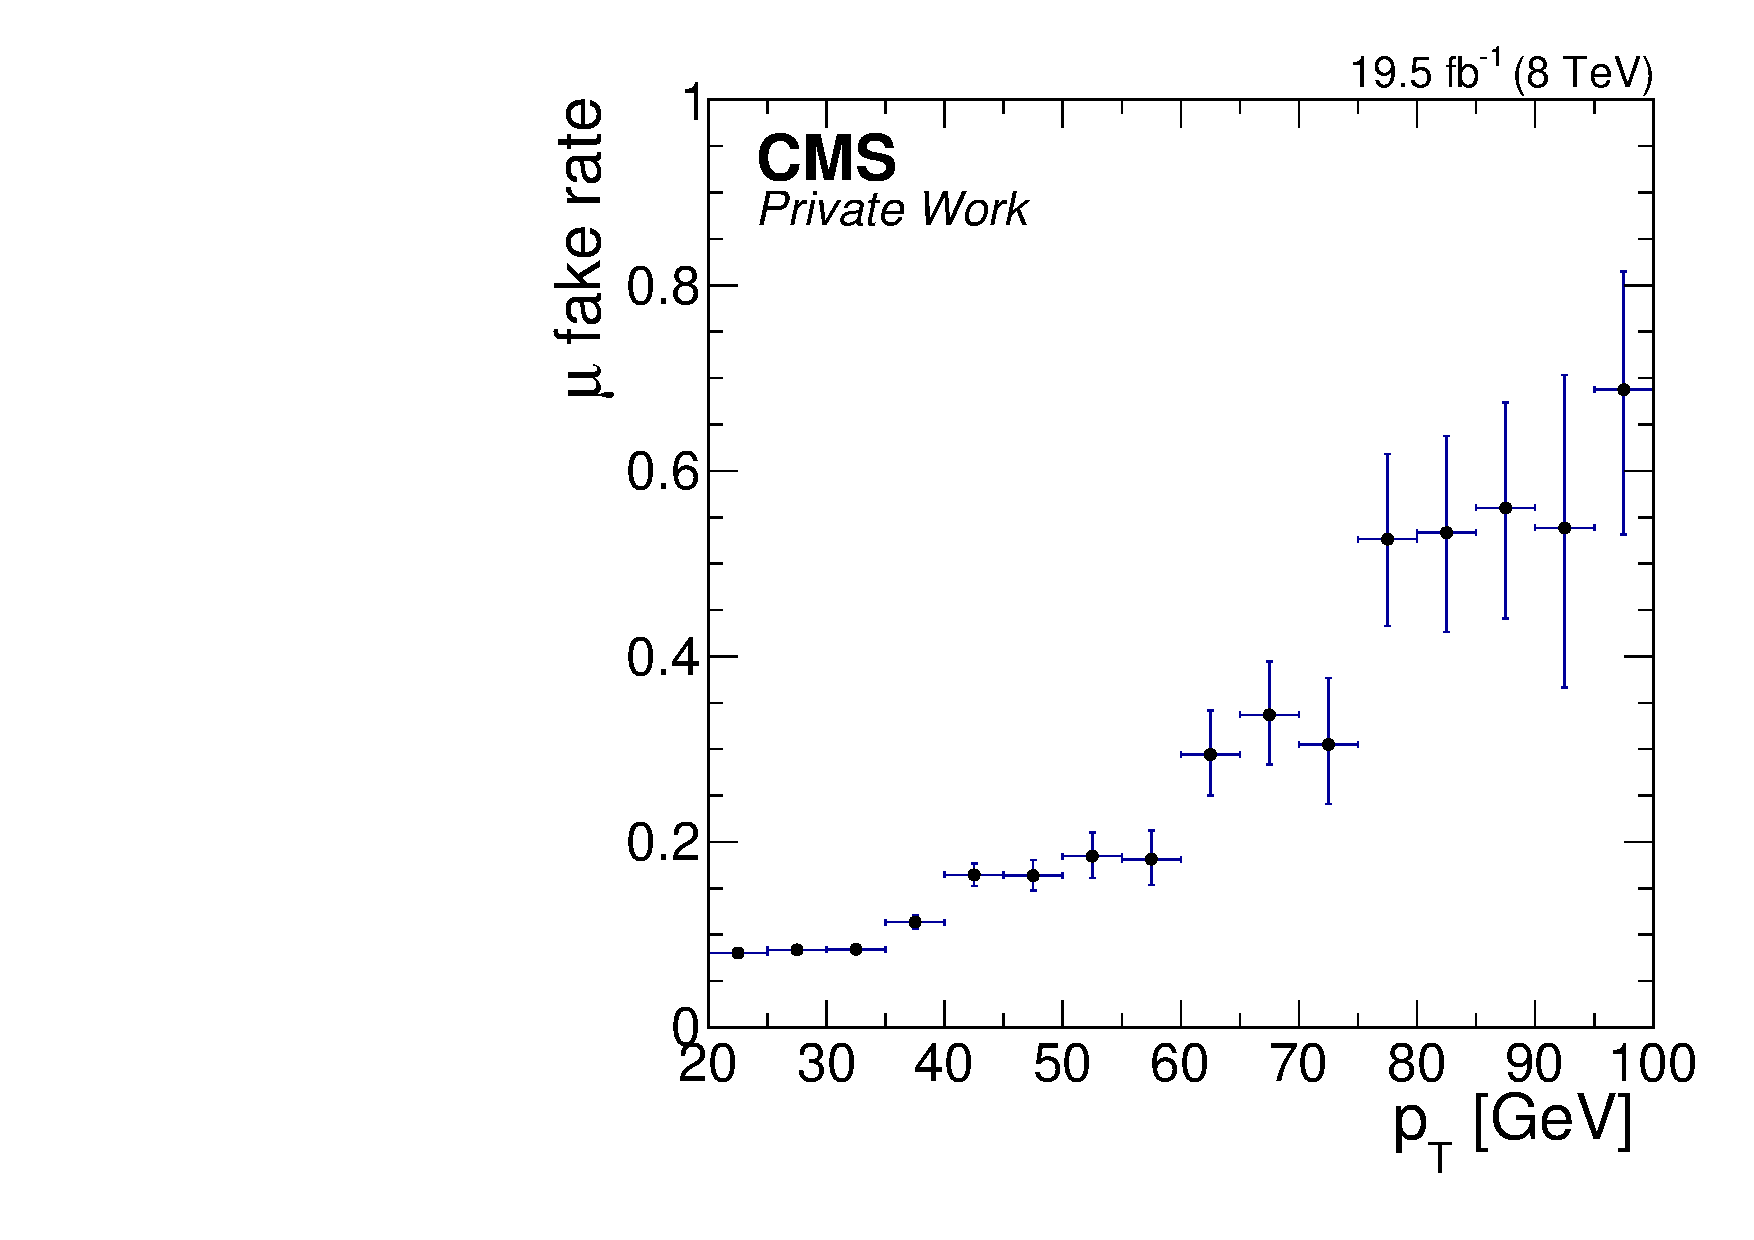
\includegraphics[width=\textwidth]{plots/BG/nonPrompt/fakeRate_mu_Inclusive_Full2012_TrailingPt_range100.pdf}
\end{minipage}
\begin{minipage}[t]{0.49\textwidth}
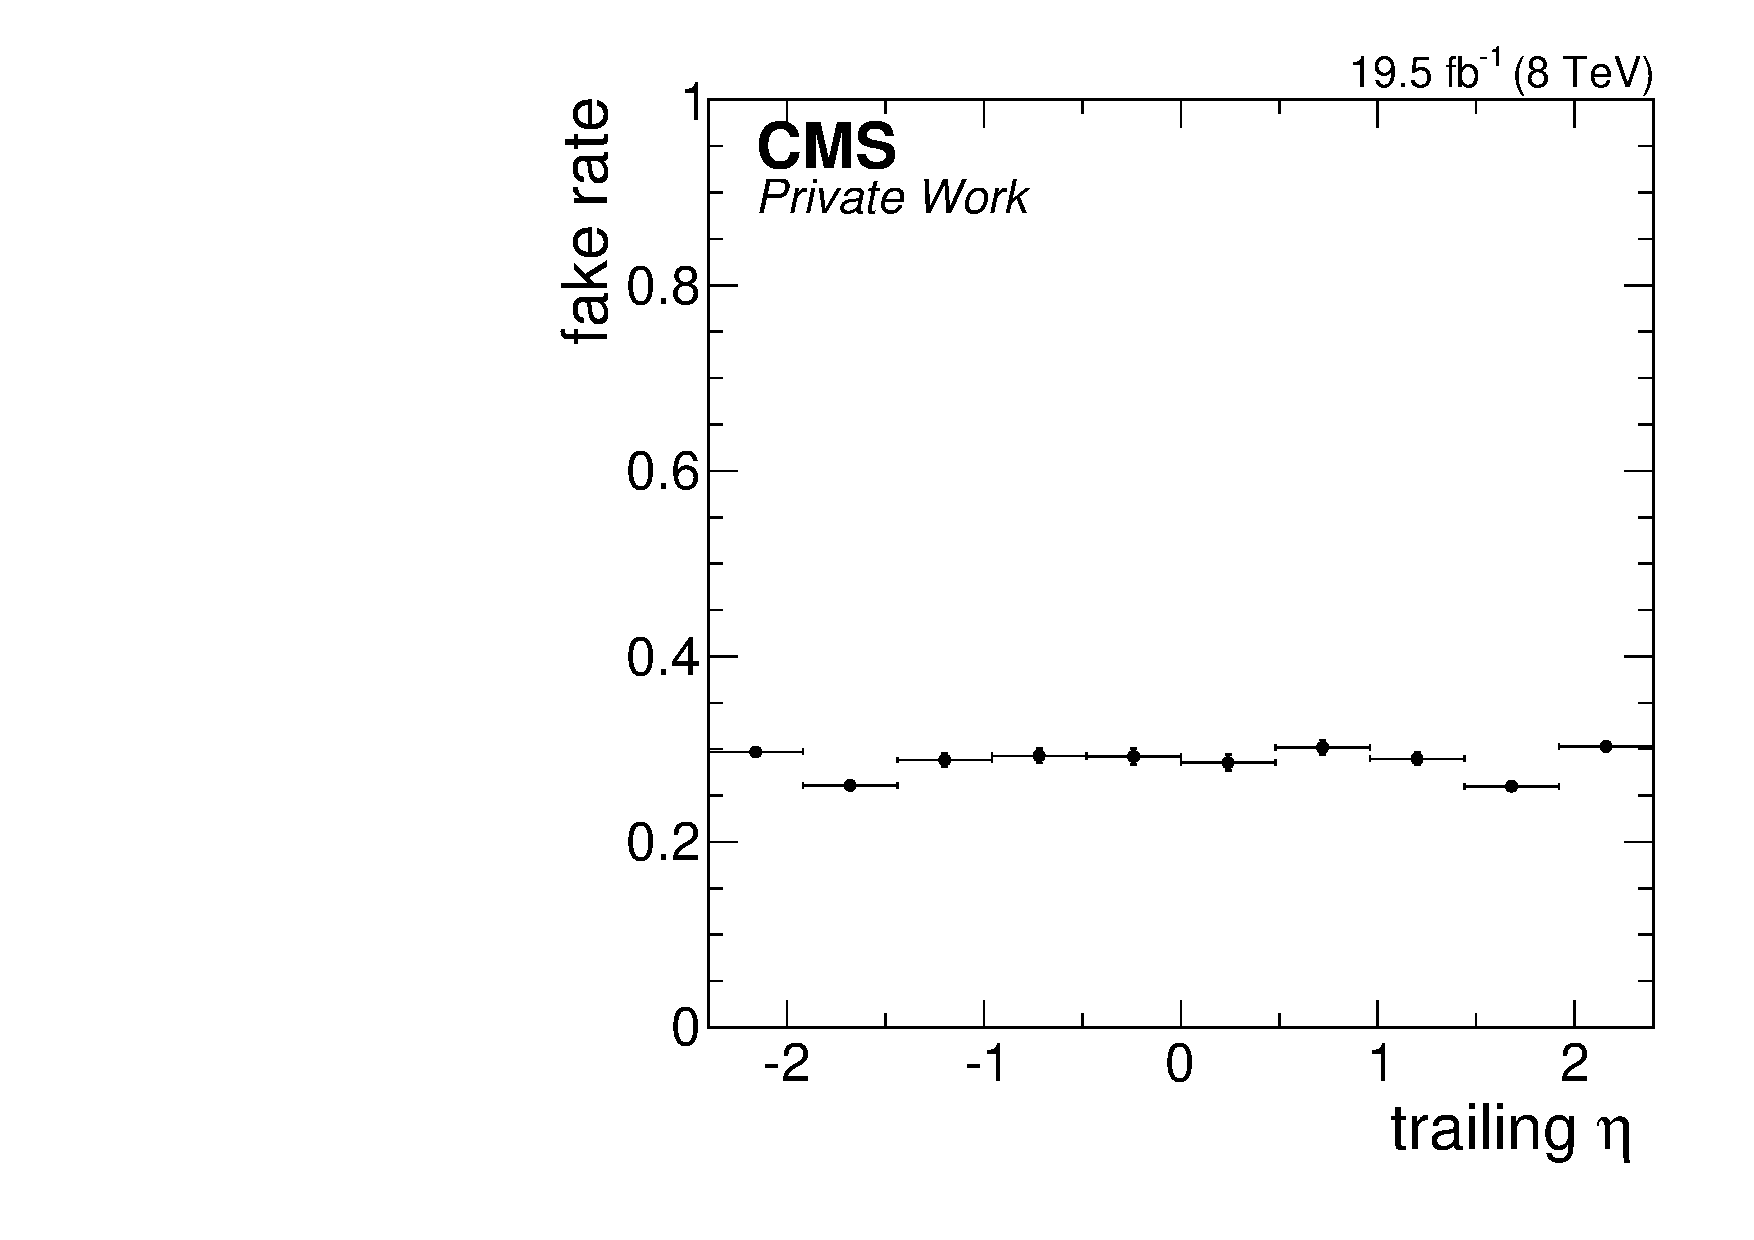
\includegraphics[width=\textwidth]{plots/BG/nonPrompt/fakeRate_ele_Inclusive_Full2012_TrailingEta_None.pdf}
\end{minipage}
\begin{minipage}[t]{0.49\textwidth}
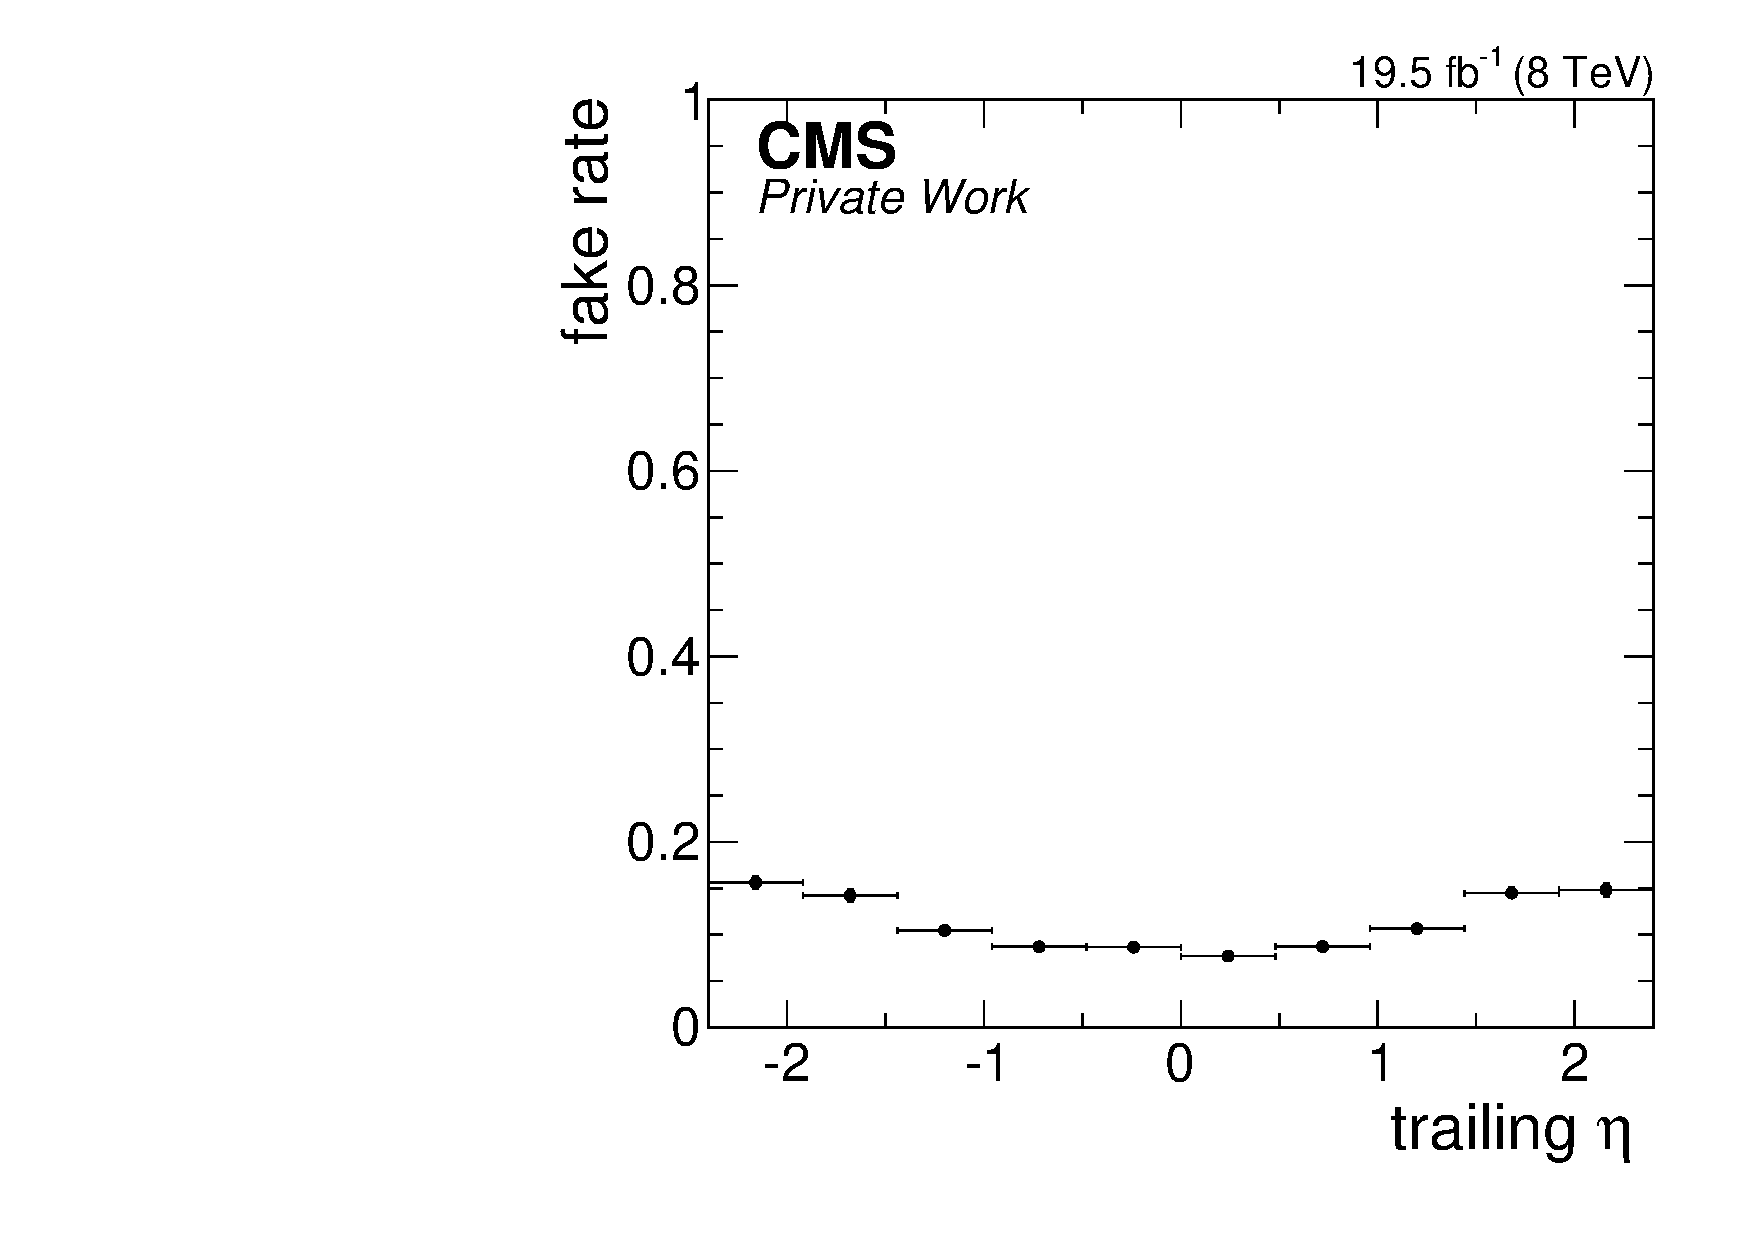
\includegraphics[width=\textwidth]{plots/BG/nonPrompt/fakeRate_mu_Inclusive_Full2012_TrailingEta_None.pdf}
\end{minipage}
\caption{Measured fake rate for electrons (left) and muons (right) as a function of the \pt (top) and $\eta$ (bottom) of the trailing lepton.}
\label{fig:fakeRate}
\end{figure} 
Similarly, to calculate the probability of a loose prompt lepton to be also a tight lepton, a sample enriched in prompt lepton is selected by requiring exactly two reconstructed leptons, of which the leading one is required to be a tight lepton which the trailing one is a loose lepton. To further enrich the sample in prompt lepton from Z boson decays, \mll is required to be within $\unit{15}{\giga\electronvolt}$ of the Z boson mass and \MET is required to be $\unit{<20}{\giga\electronvolt}$. The resulting prompt ratios $p$ are shown in Figure~\ref{fig:promptRate}. They are again applied as functions of \pt $\eta$. The systematic uncertainty assigned to the tight-to-loose ratios in the sources cited above is 50\%. As the definition of loose electrons differs from that used in said analyses and modifications have been made to the definition of the control samples in which the ratios are measured, this number is not directly applicable here. As the overall normalization of the non-prompt background is not the focus of this study, the uncertainty is increased to 100\%. 

\begin{figure}[htbp]
\centering
\begin{minipage}[t]{0.49\textwidth}
  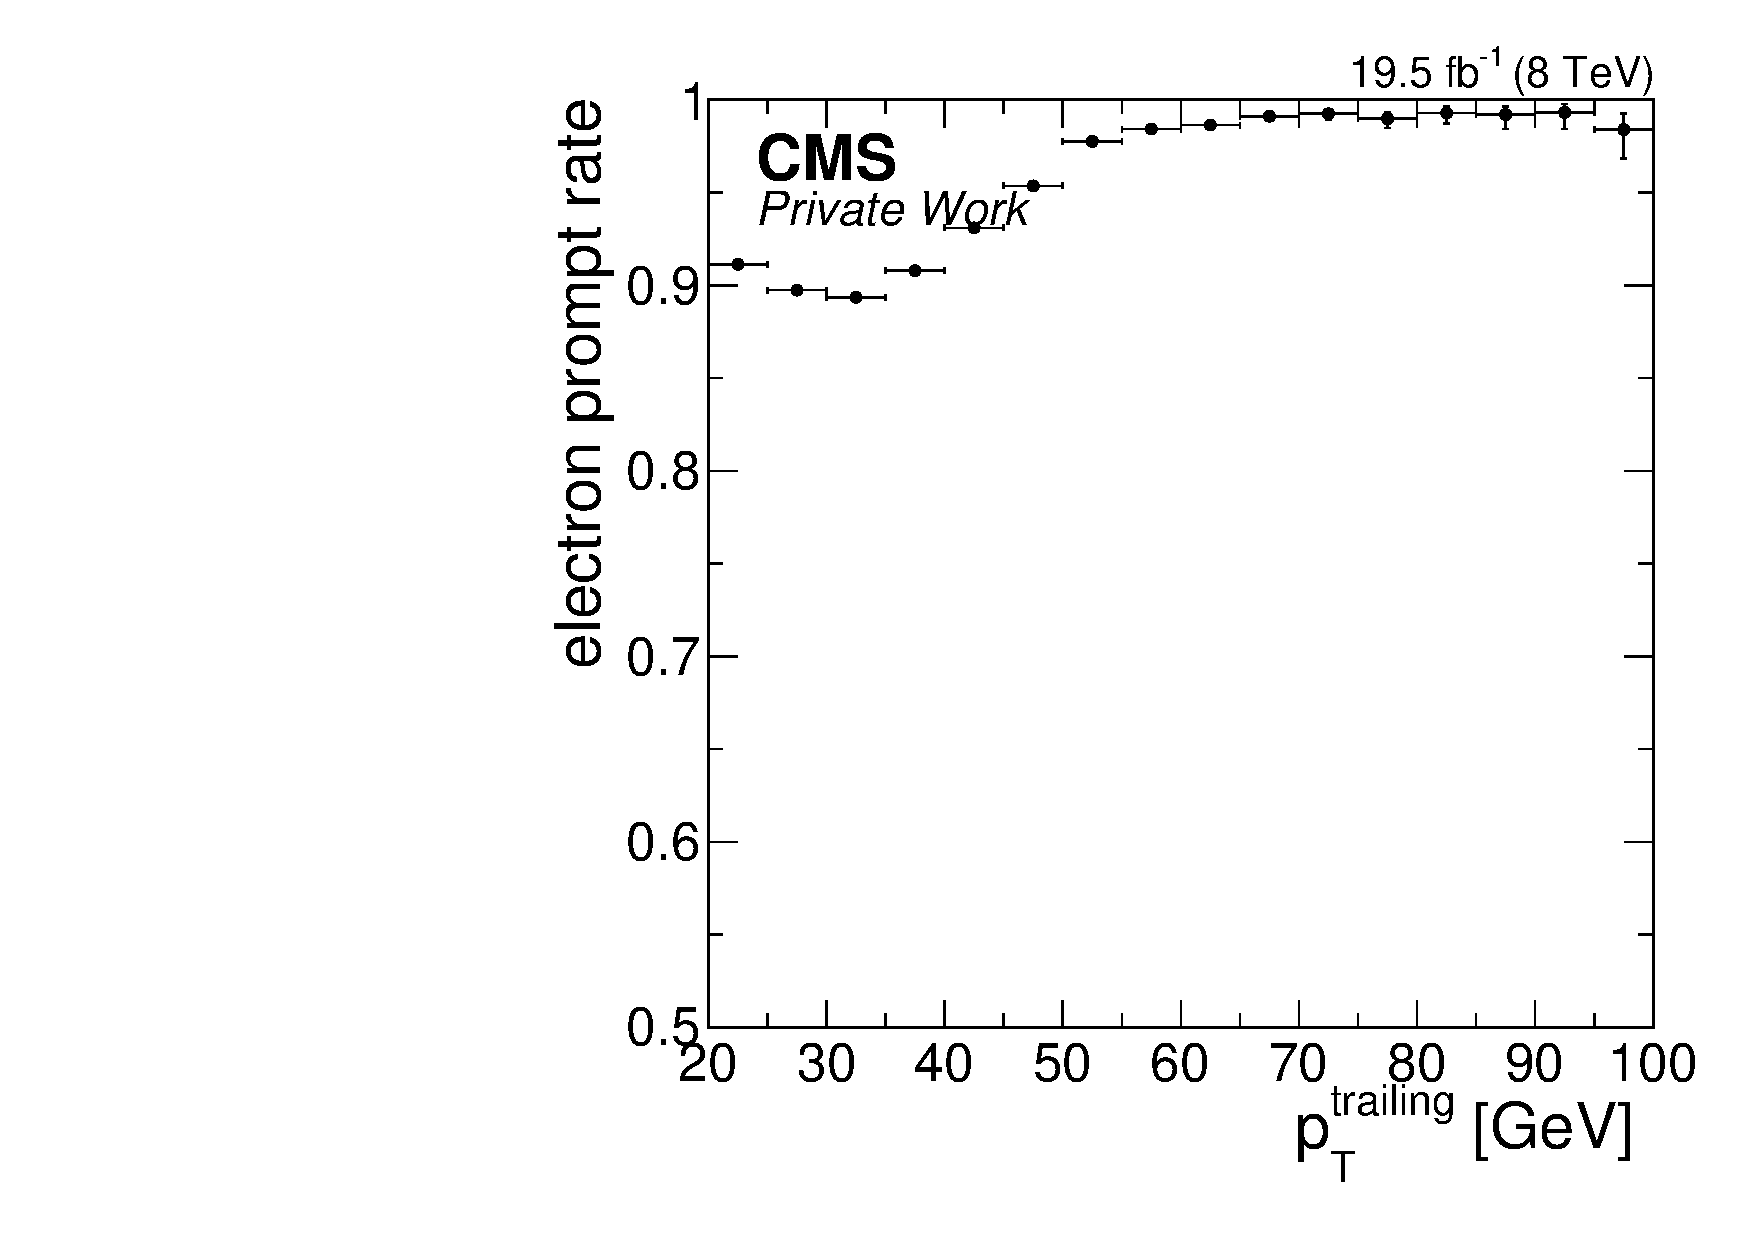
\includegraphics[width=\textwidth]{plots/BG/nonPrompt/promptRate_ele_Inclusive_Full2012_TrailingPt_range100.pdf}
\end{minipage}
\begin{minipage}[t]{0.49\textwidth}
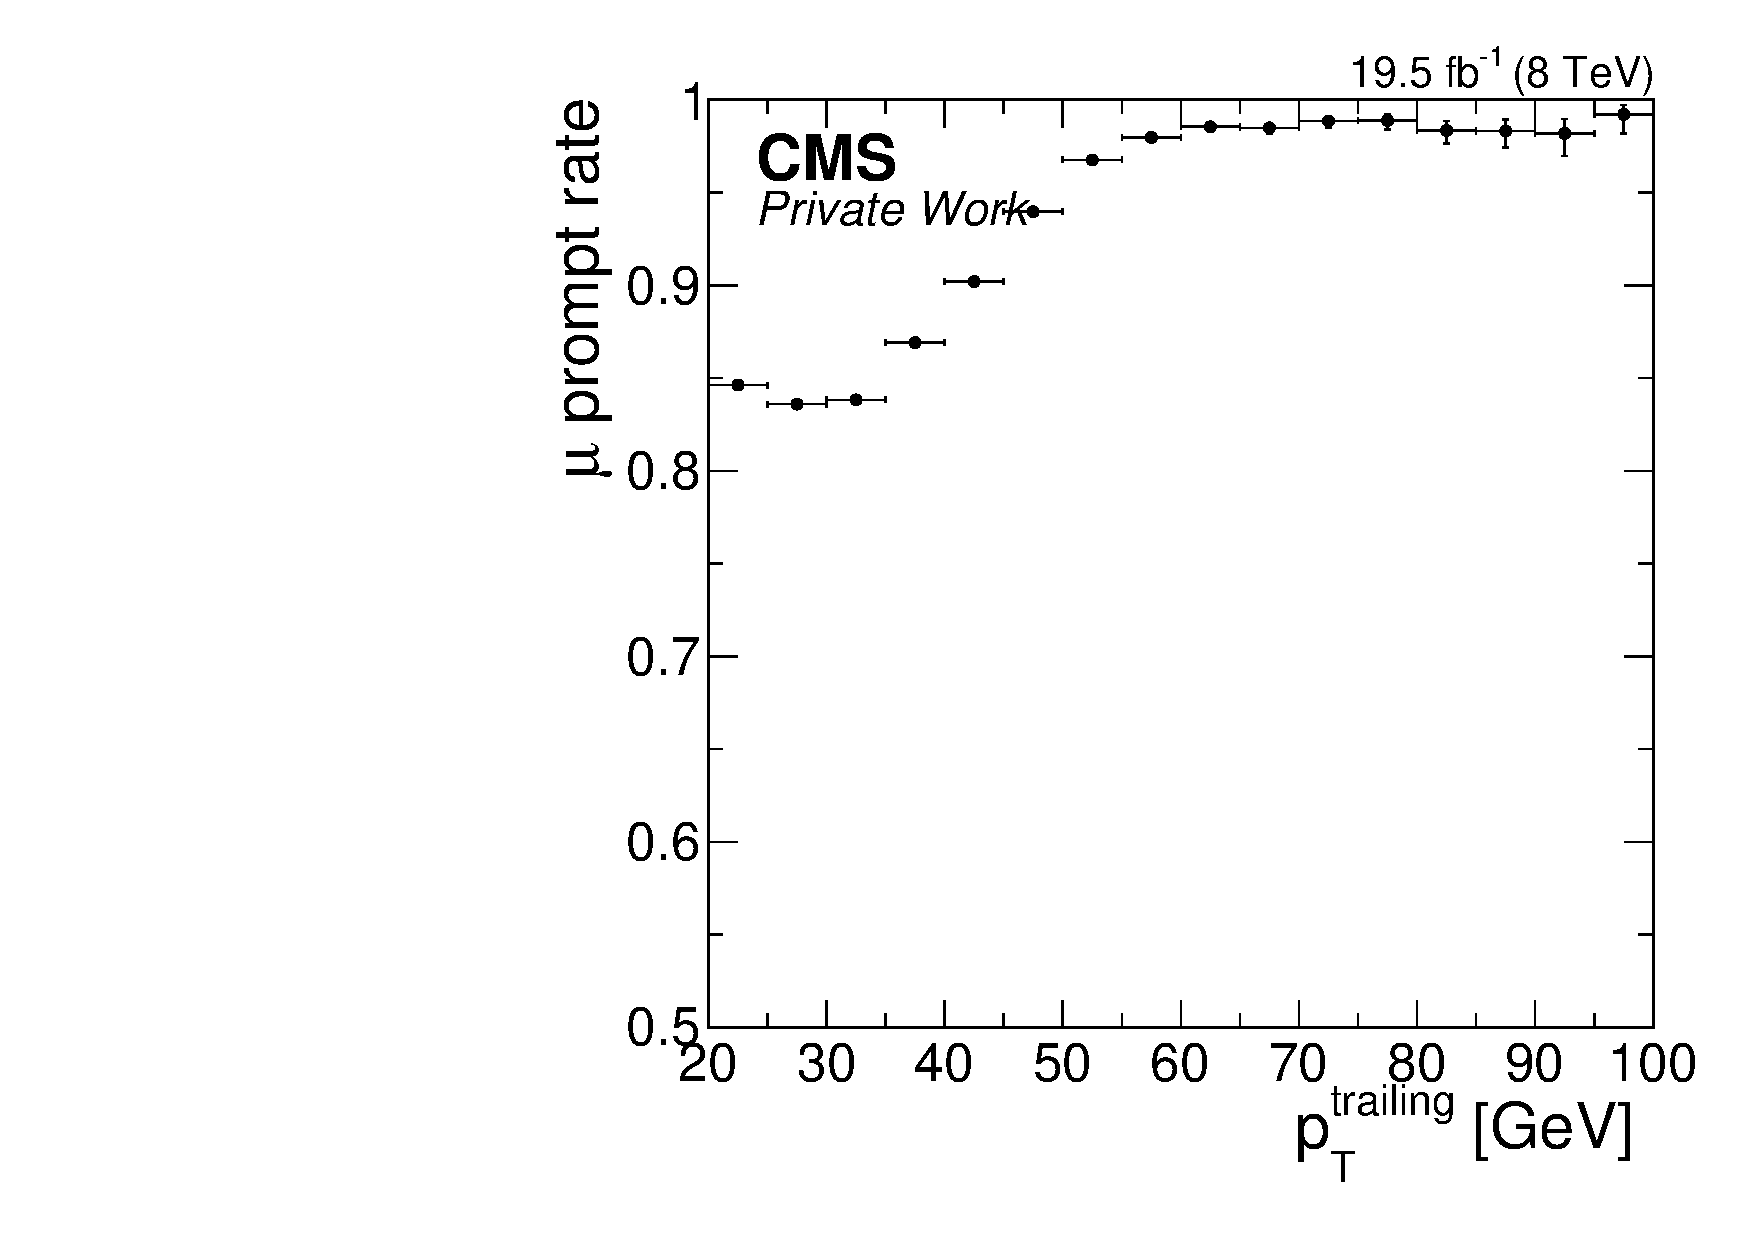
\includegraphics[width=\textwidth]{plots/BG/nonPrompt/promptRate_mu_Inclusive_Full2012_TrailingPt_range100.pdf}
\end{minipage}
\begin{minipage}[t]{0.49\textwidth}
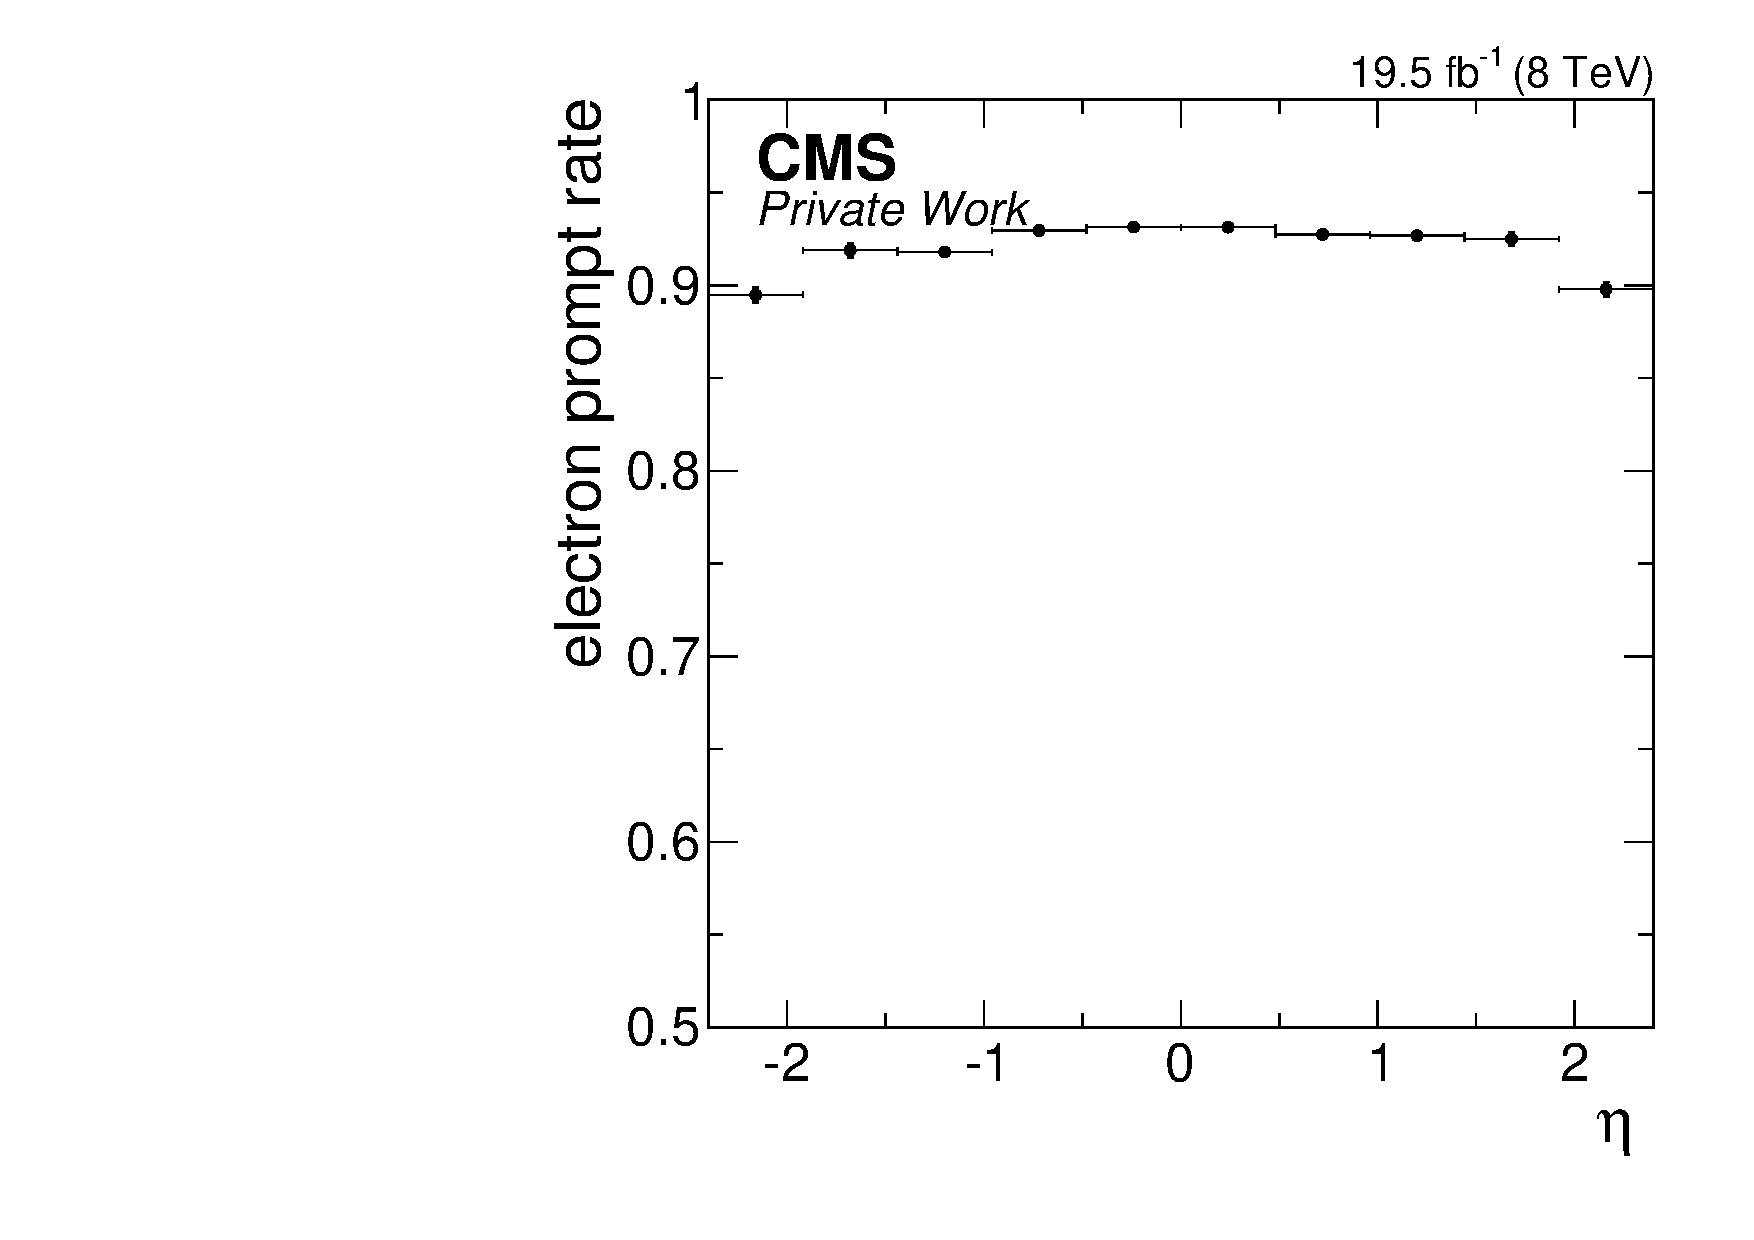
\includegraphics[width=\textwidth]{plots/BG/nonPrompt/promptRate_ele_Inclusive_Full2012_TrailingEta_None.pdf}
\end{minipage}
\begin{minipage}[t]{0.49\textwidth}
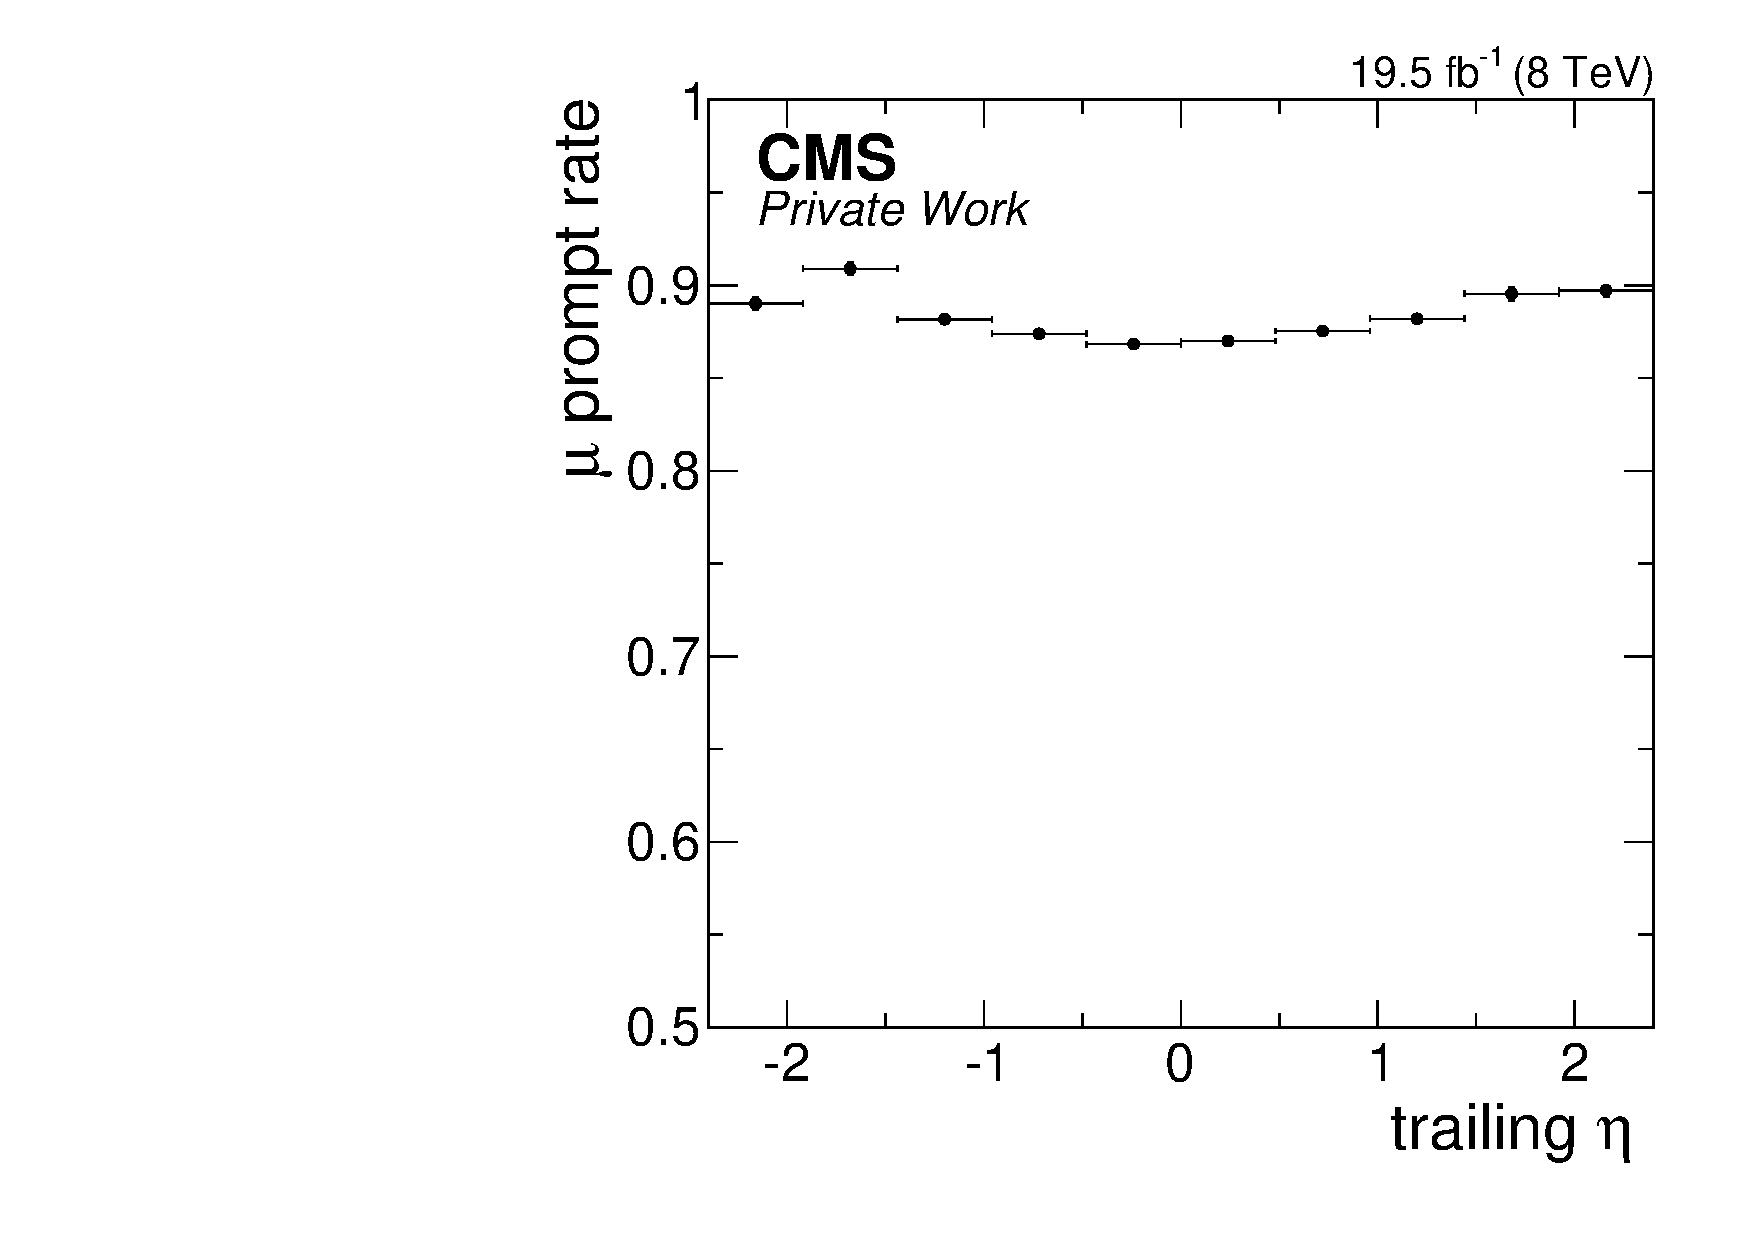
\includegraphics[width=\textwidth]{plots/BG/nonPrompt/promptRate_mu_Inclusive_Full2012_TrailingEta_None.pdf}
\end{minipage}
\caption{Measured prompt rate for electrons (left) and muons (right) as a function of the \pt (top) and $\eta$ (bottom) of the trailing lepton.}


\label{fig:promptRate}
\end{figure} 
Using the measured fake and prompt rates $f$ and $p$, the contributions of the four possible combination of prompt and non-prompt lepton (prompt-prompt, prompt-non-prompt, non-prompt-prompt, and non-prompt-non-prompt) are calculated using the following formulas
\begin{eqnarray*}
N_{pp} = N_{tt}\cdot(f_1 -1)(f2-1)p_1p_2 + N_{tl}\cdot(f_1 -1)f_2p_1p_2 + N_{lt}\cdot (f_2-1)f_1p_1p_2 + N_{ll}\cdot f_1f_2p_1p_2,\\
N_{pn} = N_{tt}\cdot(f_1 -1)(1-p_2)p_1f_2 - N_{tl}\cdot(f_1 -1)f_2p_1p_2 + N_{lt}\cdot (1-p_2)f_1p_1f_2 - N_{ll}\cdot f_1f_2p_1p_2,\\
N_{np} = N_{tt}\cdot(1 - p_1)(f_2 - 1)f_1p_2 + N_{tl}\cdot(1-p_1)f_2f_1p_2 - N_{lt}\cdot (f_2-1)f_1p_1p_2 - N_{ll}\cdot f_1f_2p_1p_2,\\
N_{nn} = N_{tt}\cdot(1-p_1)(1-p_2)f_1f_2 - N_{tl}\cdot (1-p_1)f_2f_1p_2 - N_{lt}\cdot (1-p_2)f_1p_1f_2 + N_{ll}\cdot f_1f_2p_1p_2,\\
\end{eqnarray*}
where each of the contributions has to be weighted by $(f_1-p_1)(f_2-p_2)$. As the fake and prompt rates depend on \pt and $\eta$ of the leptons, in practice each event is assigned a weight based on whether the leptons are tight and loose and their kinematic properties according to the formulas above. The estimates for $N_{pp}$, $N_{pn}$, $N_{np}$, and $N_{nn}$ are obtained as the sum of these weights. The total contribution of non-prompt backgrounds is than given by the sum of $N_{pn}$, $N_{np}$, and $N_{nn}$. The resulting estimates in the central and forward signal regions are shown in Table~\ref{tab:nonPromptTable}. 

\begin{table}[!htbp]
 \renewcommand{\arraystretch}{1.2}
 \begin{center}
  \caption{Results of the estimation of backgrounds with non-prompt leptons in the signal region using the tight-to-loose ratios for prompt and non-prompt leptons. The total non-prompt estimate is given by the sum of the contributions for events with one or two non-prompt leptons $N_{pp}$, $N_{np}$, and $N_{pn}$.}
  \begin{tabular}{l|ccccc}

                                    & \EE & \MM & SF & \EM          \\
   \hline
   & \multicolumn{4}{c}{Signal central} \\
   \hline
       $N_{tt}$      &  1257  & 1450 & 2707  & 2326             \\
       $N_{lt}$ + $N_{tl}$      &  247  & 740 & 987  & 812             \\
       $N_{ll}$      &  11  & 114 & 125  & 50             \\

\hline
       Non-prompt estimate      &  44.9$\pm$14.8  & 34.6$\pm$3.8 & 79.6$\pm$18.6  & 86.7$\pm$12.4             \\

\hline
\hline
   
   & \multicolumn{4}{c}{Signal forward} \\
   \hline
       $N_{tt}$      &  405  & 473 & 878  & 827             \\
       $N_{lt}$ + $N_{tl}$      &  130  & 233 & 363  & 234             \\
       $N_{ll}$      &  6  & 38 & 44  & 32             \\

\hline
       Non-prompt estimate      &  27.3$\pm$8.0  & 17.9$\pm$3.5 & 45.1$\pm$11.5  & 43.4$\pm$8.4             \\

 \end{tabular}
 \label{tab:nonPromptTable}
 \end{center}
\end{table}

It can be seen that the contribution of non-prompt leptons is small compared to the total number of tight lepton pairs and that the estimates are well compatible between SF and OF events within the statistical uncertainties. This type of backgrounds is therefore accounted for by the background estimates for flavour-symmetric backgrounds.
\section{Backgrounds containing a Z boson}
To estimate the contribution of backgrounds containing a Z boson to the event sample in the signal region, both the Jet-Z-balance (JZB) and \MET templates methods~\cite{Chatrchyan:2012qka} are used. The first studies the balance of the Z boson against the jets in the event. In the \MET template method, the \MET distribution of $\gamma$+jets events are used to estimate that of Z+jets events. As the development and application of these methods have not been part of the work covered in this thesis, only a short description will be given.
\subsection{JZB method}
The \JZB variable is defined as the balance of the \pt of the jets in the event with the \pt of the Z candidate. To avoid biases due to jet selection, \METVec is used as a measure of the hadronic recoil of the \Z:
\begin{equation}
\JZB = | \sum\limits_{\mathrm{jets}}\vec{p}_{\mathrm{T}}| - | \vec{p}_{\mathrm{T}}^{\text{ }\mathrm{Z}}| \approx | \vec{E}_{\mathrm{T}}^{\mathrm{miss}} -  \vec{p}_{\mathrm{T}}^{\text{ }\mathrm{ Z}}| - |\vec{p}_{\mathrm{T}}^{\text{ }\mathrm{Z}}| .
\end{equation}
For SM processes such as \zjets, where \MET is caused by mismeasurements of the jets, the \JZB distribution is symmetric around 0. For BSM processes, where the \Z boson is produced correlated with invisible particles, the \JZB distribution is expected to be asymmetric, favouring positive sign especially for large values of \JZB and by extension high \MET. Therefore it is possible to predict the contribution of SM processes containing a \Z boson at high \MET from the events in that region with negative values of \JZB, after subtraction of flavour-symmetric processes from OF events. The assumption that the \JZB distribution is symmetric around 0 for SM processes with only instrumental \MET is studied in MC and 20\% systematic uncertainty are assigned.\fixme{Add reference to 2012 paper}.
\subsection{\MET templates method}
The \MET templates method utilizes the similarity of \zjets and \gjets events, especially mismeasurement as only source of \MET. Therefore, after corrections for residual kinematic differences, the contribution of \zjets events at high \MET can be estimated from \gjets events passing the same selection. The dominant systematic uncertainties are assigned based on tests of the method on simulation and are in the order of 15-100\% for \MET values falling into the signal selection of this analysis. The large uncertainties for higher \MET values are driven the available MC statistics to validate the method. 

In contrast to the \JZB method, the \MET templates method does account only for \zjets events. Other backgrounds containing \Z bosons, such as WZ, ZZ or more rare SM processes like $t\bar{t}Z$ or Triboson production are estimated from simulation and assigned 50\% uncertainty. 
\subsection{Extrapolation for off-Z regions}
Both methods described above result in background estimates for the on-\Z region of 81\GeV $< \mll < $ 101\GeV. Contributions to the low-Mass and high-Mass selections from off-Shell \Z bosons or the Drell--Yan continuum are estimated by applying an extrapolation factor \Routin to the on-Z prediction. \Routin is measured in the Drell--Yan control region, separately for the low-Mass and high-Mass region as well as \EE, \MM and SF leptons. It is defined as the ratio of the event yield in the mass region in question (\textit{out}) by that in the on-Z mass region (\textit{in}), after subtraction of contribution from flavour-symmetric processes from the OF sample:
\begin{equation}
\Routin = \frac{\mathrm{N}_{\mathrm{out}}^{\mathrm{SF}} - \mathrm{N}_{\mathrm{out}}^{\mathrm{OF}}\Rsfof}{ \mathrm{N}_{\mathrm{in}}^{\mathrm{SF}} - \mathrm{N}_{\mathrm{in}}^{\mathrm{OF}}\Rsfof},
\end{equation} 
where the SF is substituted for \EE or \MM according to the desired lepton flavour. The \mll distribution in the Drell--Yan control region is shown in Figure~\ref{fig:rOutIn}. The resulting values range from about 6-8\% for the low-Mass region to 2-3\% for the high-Mass region, as summarized in Table~\ref{tab:rOutIn}.
\begin{figure}[htbp]
\centering
\begin{minipage}[t]{0.49\textwidth}
  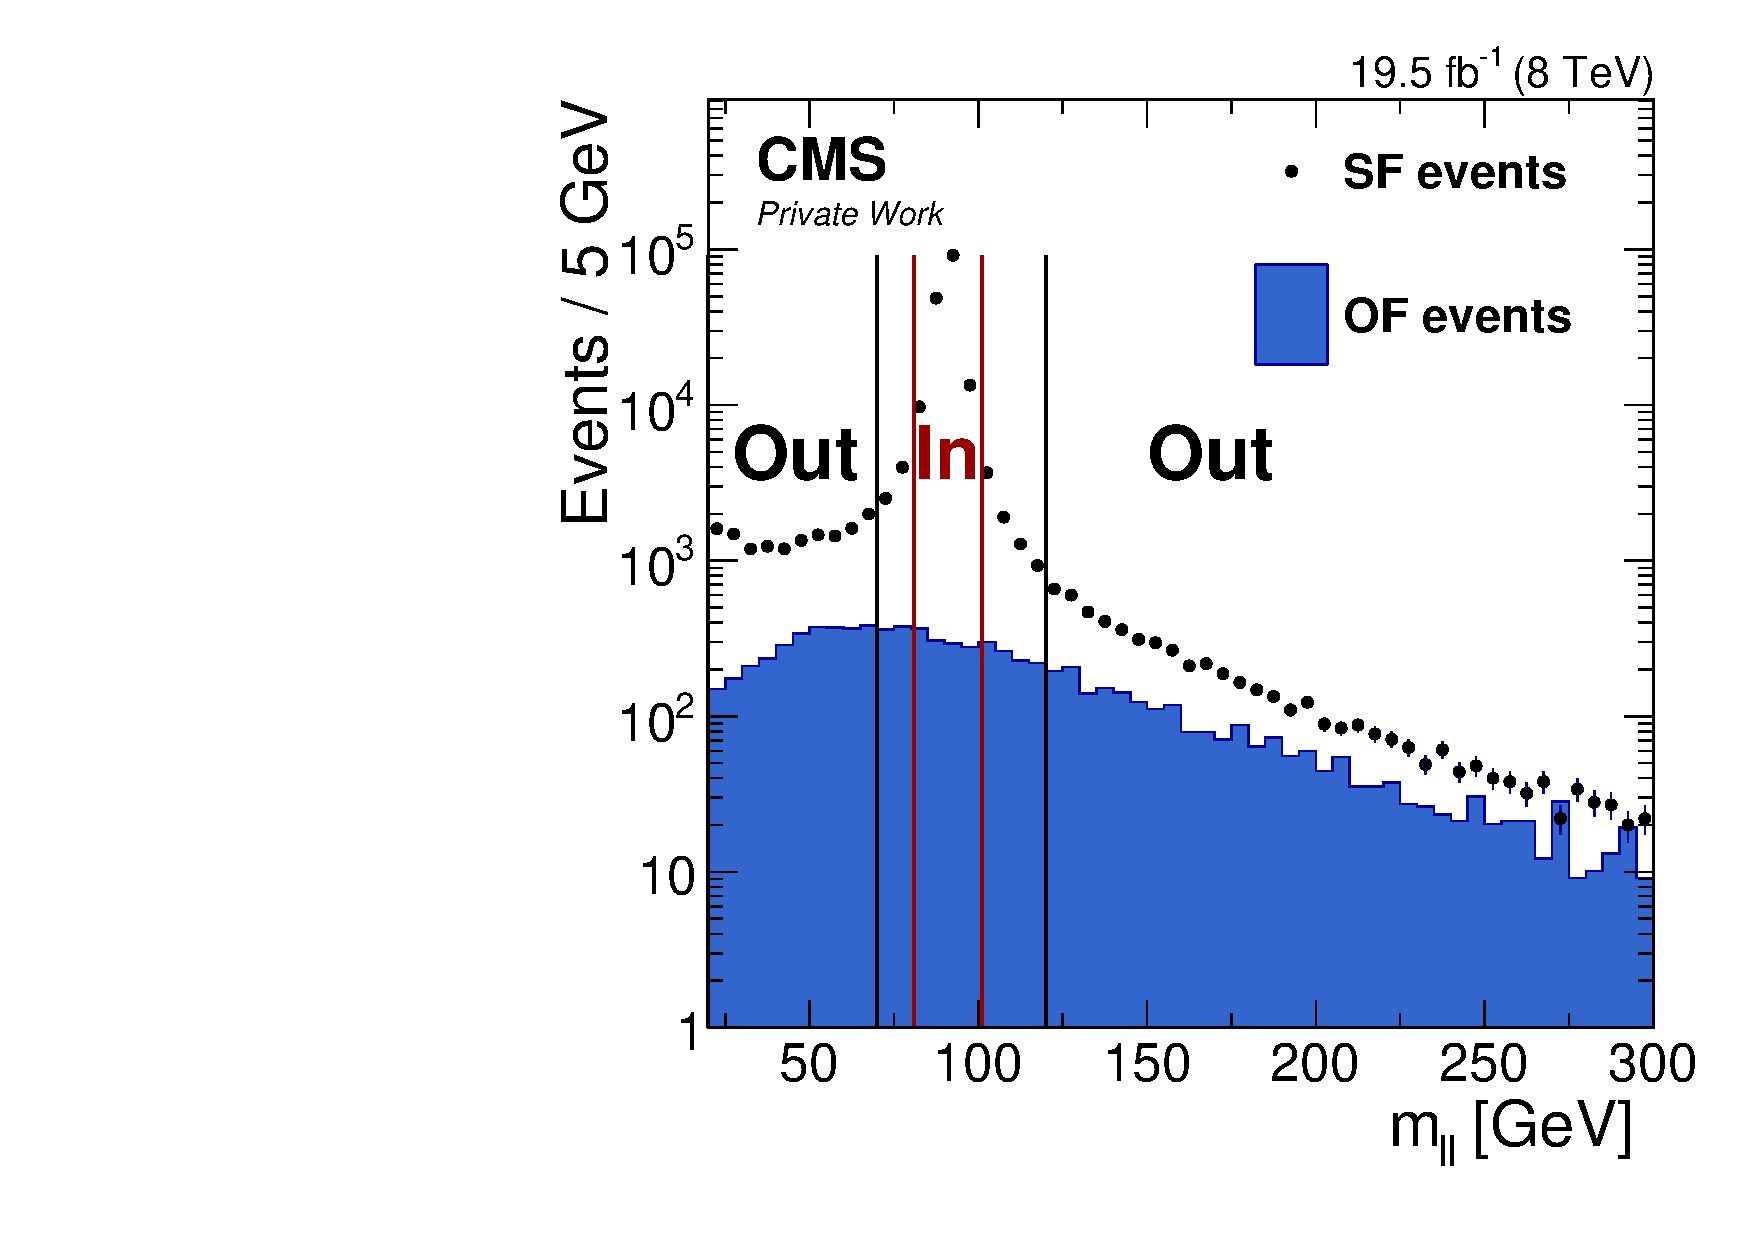
\includegraphics[width=\textwidth]{plots/BG/rOutIn/rOutIn_SF_DrellYanControlCentral_Full2012.pdf}
\end{minipage}
\begin{minipage}[t]{0.49\textwidth}
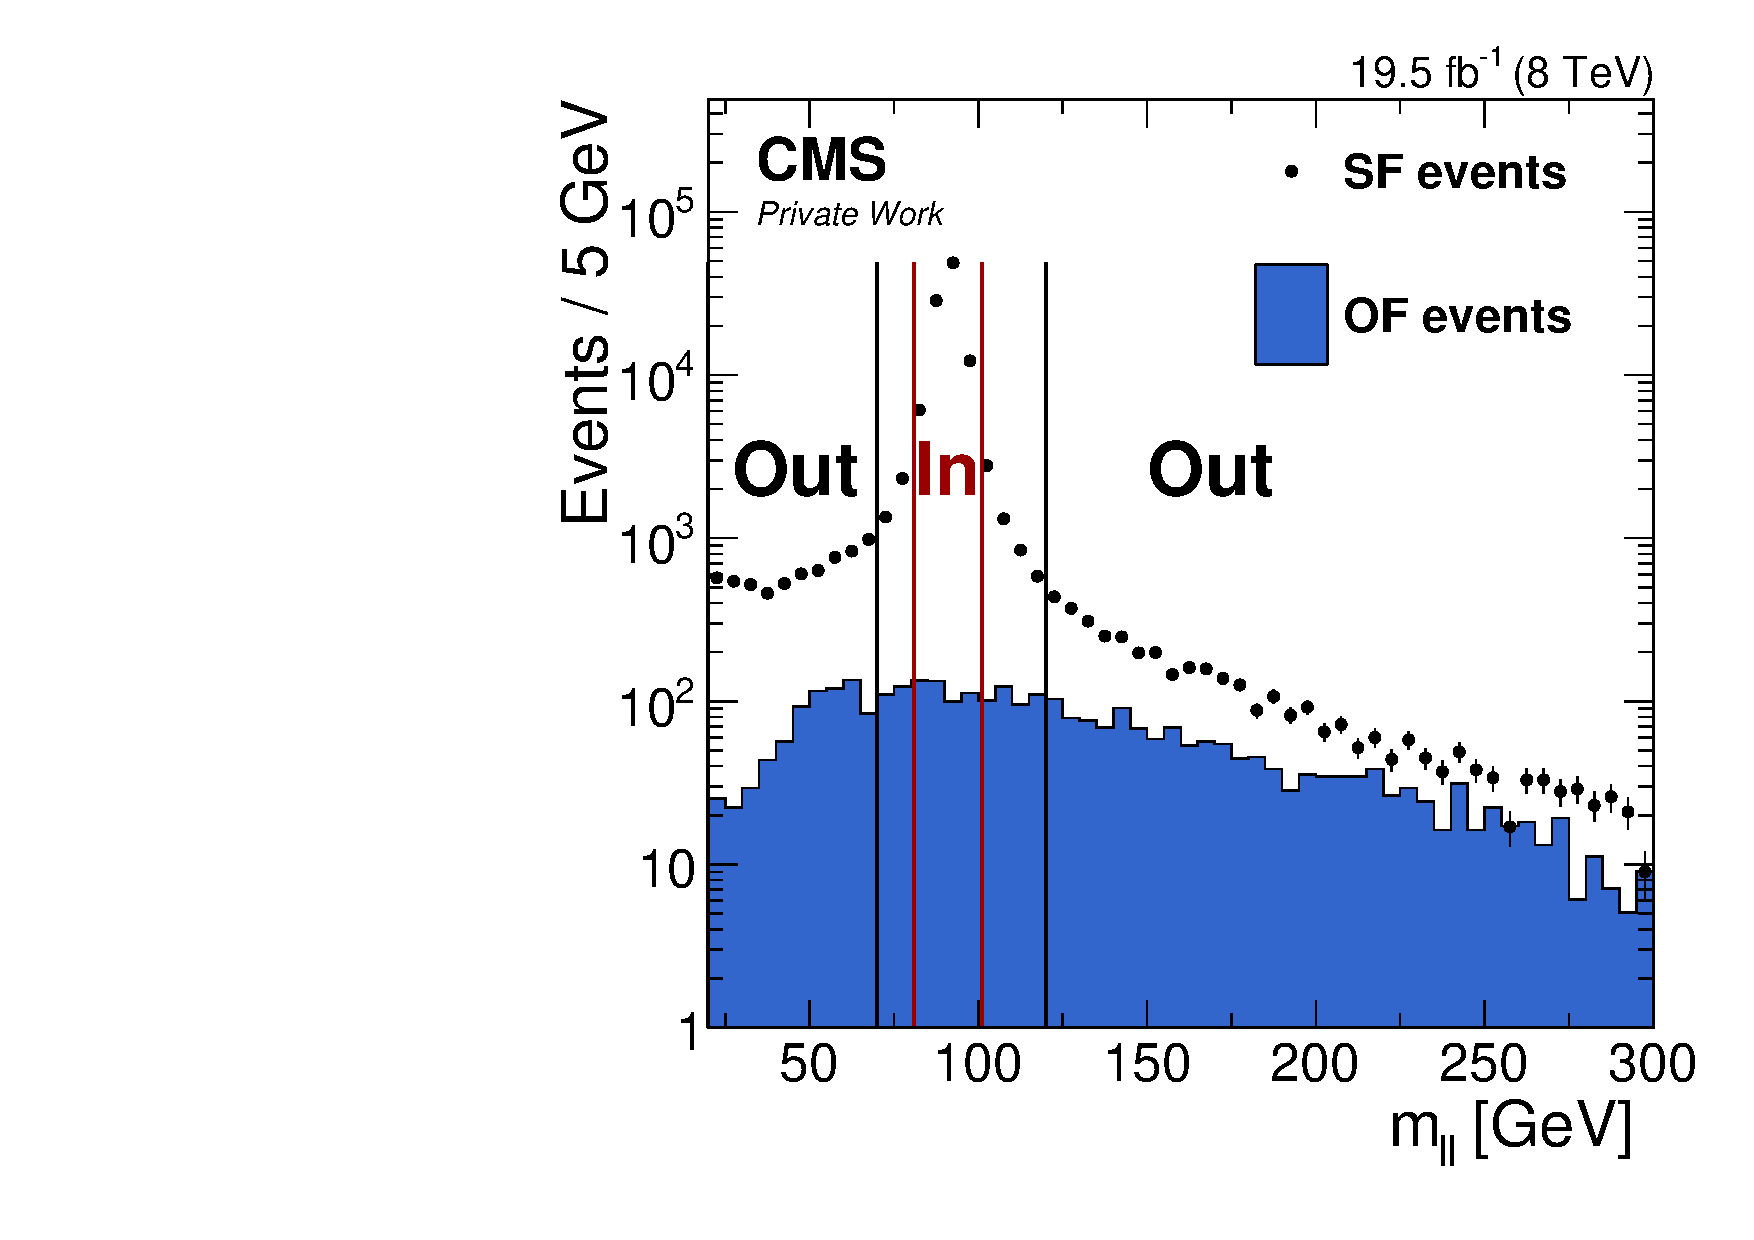
\includegraphics[width=\textwidth]{plots/BG/rOutIn/rOutIn_SF_DrellYanControlForward_Full2012.pdf}
\end{minipage}

\caption{The \mll distribution in the Drell--Yan control region in the central (left) and forward (right) dielepton selection. SF data is shown as the black points while OF data is shown as the blue histogram. The black lines indicate the boundaries of the two \textit{out} regions and the dark red lines those of the \textit{in} region.}
\label{fig:rOutIn}
\end{figure} 

\begin{table}[hbtp]
 \renewcommand{\arraystretch}{1.3}
 \setlength{\belowcaptionskip}{6pt}
 \centering
 \caption{
     }
  \label{tab:rOutIn}
\begin{tabular}{l|c|c|c}     
 & $N_{\text{out}}$ & $N_{\text{in}}$ & $ \Routin (SF) \pm \sigma_{stat}$  \\    
\hline
 & \multicolumn{3}{c}{Central} \\
\hline 
 & \multicolumn{3}{c}{Low mass}   \\ 
  Data & 11608.6$\pm$131.7 & 160645.8$\pm$403.9 & 0.072$\pm$0.001$\pm$0.018 \\
 MC & 10725.8$\pm$128.7 & 167291.6$\pm$412.0 & 0.064$\pm$0.001$\pm$0.016 \\

\hline 
& \multicolumn{3}{c}{high Mass} \\ 
\hline
 Data & 3571.3$\pm$91.2 & 160645.8$\pm$403.9 & 0.022$\pm$0.001$\pm$0.006 \\
 MC & 3243.0$\pm$88.9 & 167291.6$\pm$412.0 & 0.019$\pm$0.001$\pm$0.005 \\

 
    \hline 
& \multicolumn{3}{c}{Forward} \\
\hline 
 & \multicolumn{3}{c}{Low mass}   \\ 
  Data & 5657.6$\pm$84.2 & 94407.6$\pm$308.7 & 0.060$\pm$0.001$\pm$0.015 \\
 MC & 5695.8$\pm$85.5 & 103407.4$\pm$323.0 & 0.055$\pm$0.001$\pm$0.014 \\

\hline 
& \multicolumn{3}{c}{high Mass} \\ 
\hline
 Data & 2672.5$\pm$75.8 & 94407.6$\pm$308.7 & 0.028$\pm$0.001$\pm$0.007 \\
 MC & 2459.1$\pm$72.3 & 103407.4$\pm$323.0 & 0.024$\pm$0.001$\pm$0.006 \\


  
\end{tabular}  
\end{table}

The validity of applying the \Routin as measured in the Drell--Yan control region in the signal region is checked by studying the behaviour of the quantity as a function of \MET and \njets. The results for the low-Mass selection and the case of SF leptons is shown in Figure~\ref{fig:ROutInDependencies} for both the central and forward lepton selections. In neither selection a clear dependency on \MET is observed. However, above 70\GeV there is not enough statistics left after subtraction of the flavour-symmetric backgrounds, so it is not possible to judge the behaviour all the way up to the signal region. The value of \Routin clearly increases with the number of jets. As the requirement on \njets is the same between the Drell--Yan control region and the signal region, the events do not differ much in terms of jet multiplicity and this dependency does not significantly restrict the applicability of the \Routin factors in the signal region. In total, an systematic uncertainty of 25\% is assigned to cover the observed effects. Consistent results are observed also for the high-Mass region and for the split into \EE and \MM, as can be seen in Appendix~\fixme{Make routin appendix and refer to it.}

\begin{figure}[htbp]
\centering
\begin{minipage}[t]{0.49\textwidth}
  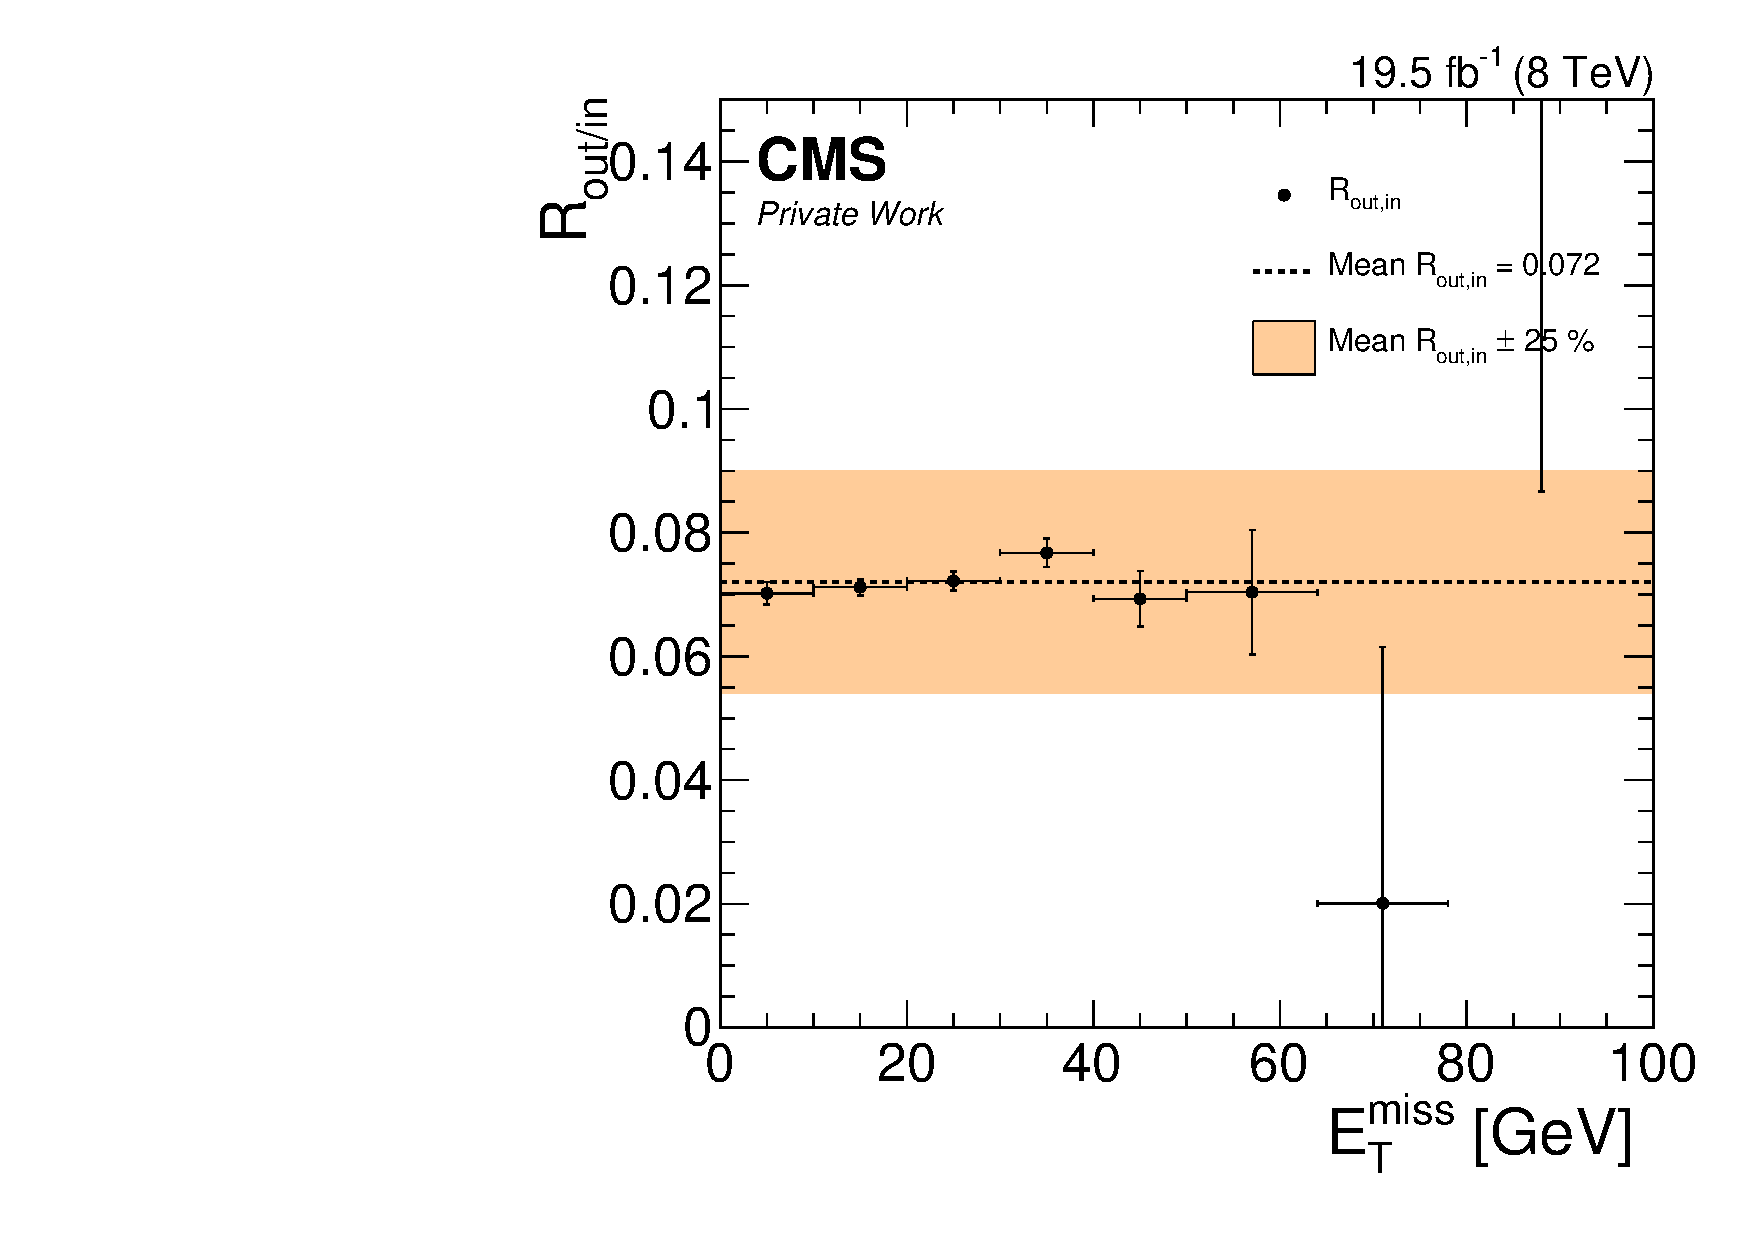
\includegraphics[width=\textwidth]{plots/BG/rOutIn/rOutInSyst_DrellYanControlCentral_Full2012_MET_LowMass_SF_None.pdf}
\end{minipage}
\begin{minipage}[t]{0.49\textwidth}
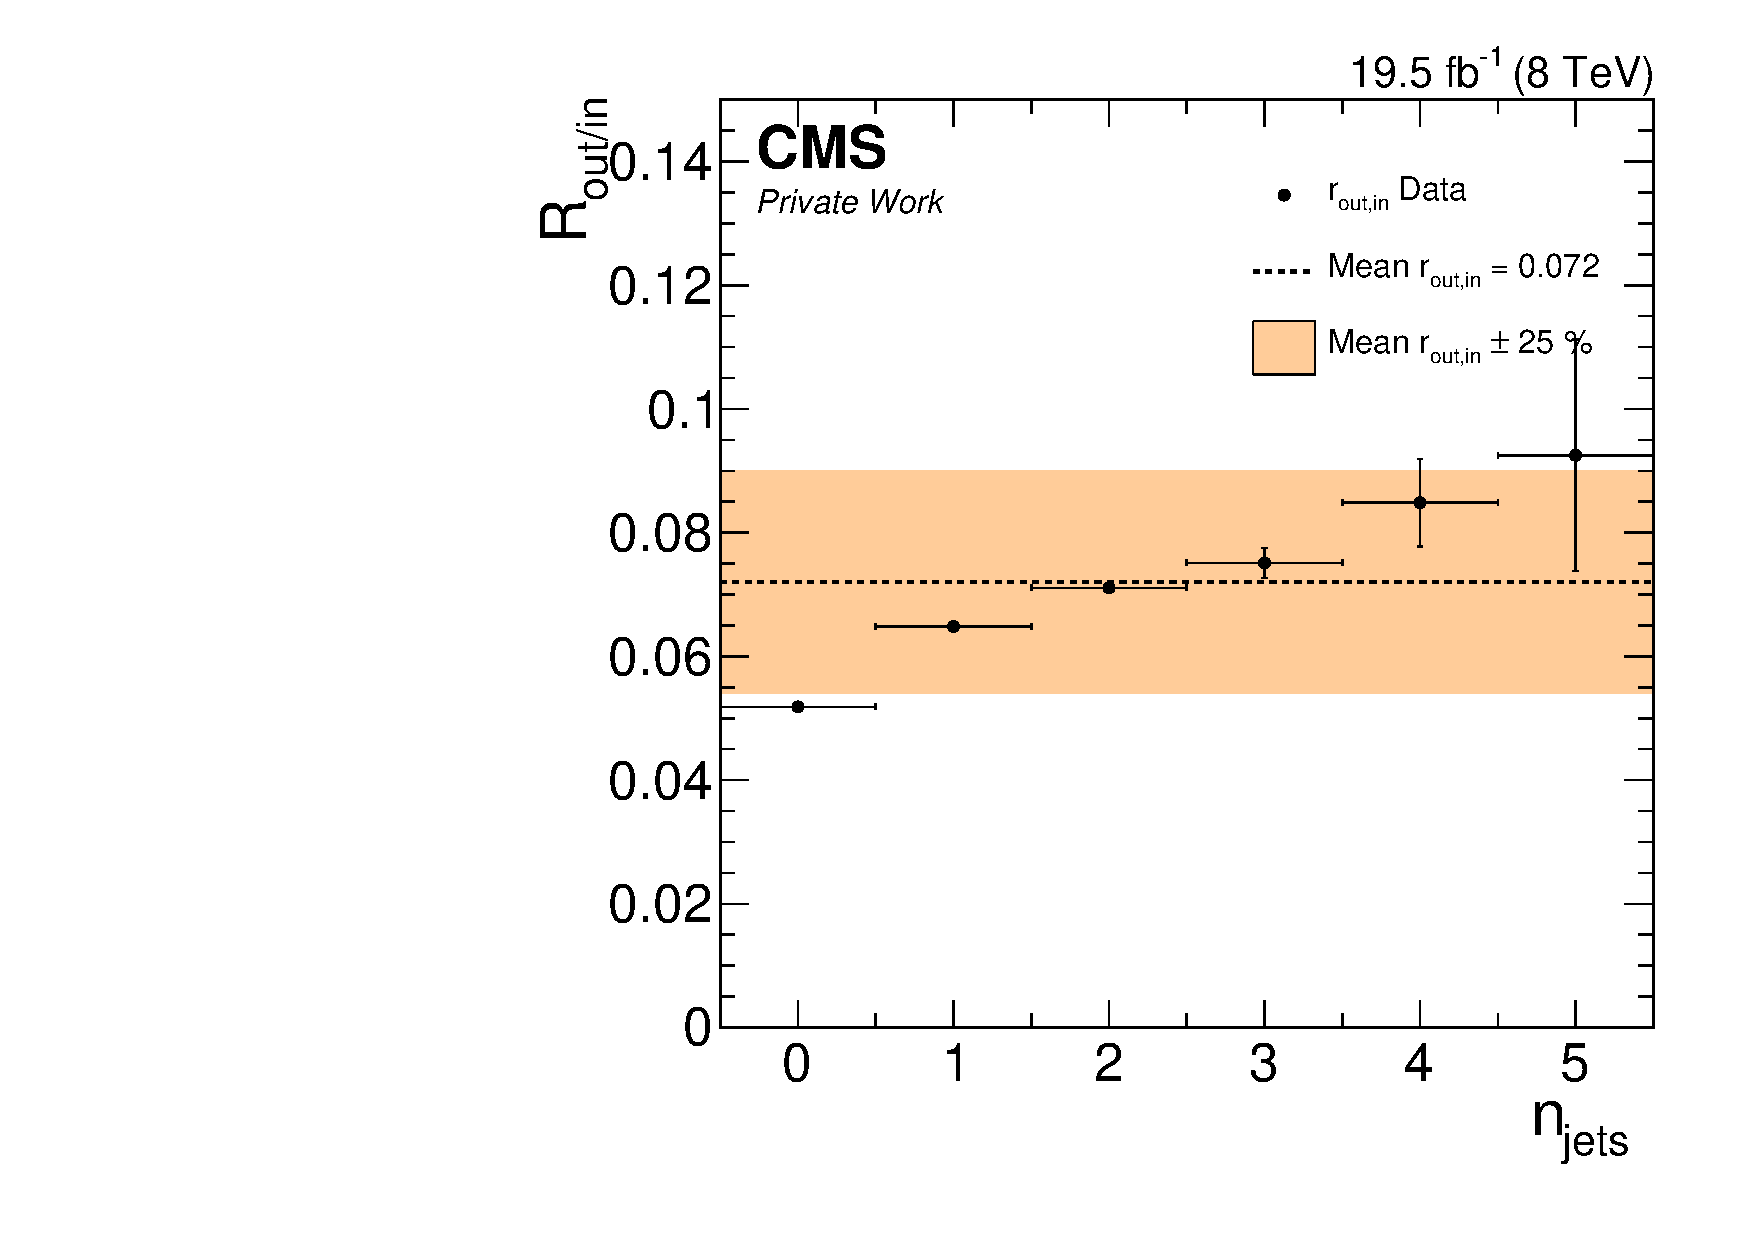
\includegraphics[width=\textwidth]{plots/BG/rOutIn/rOutInSyst_DrellYanControlCentral_Full2012_NJets_LowMass_SF_None.pdf}
\end{minipage}
\begin{minipage}[t]{0.49\textwidth}
  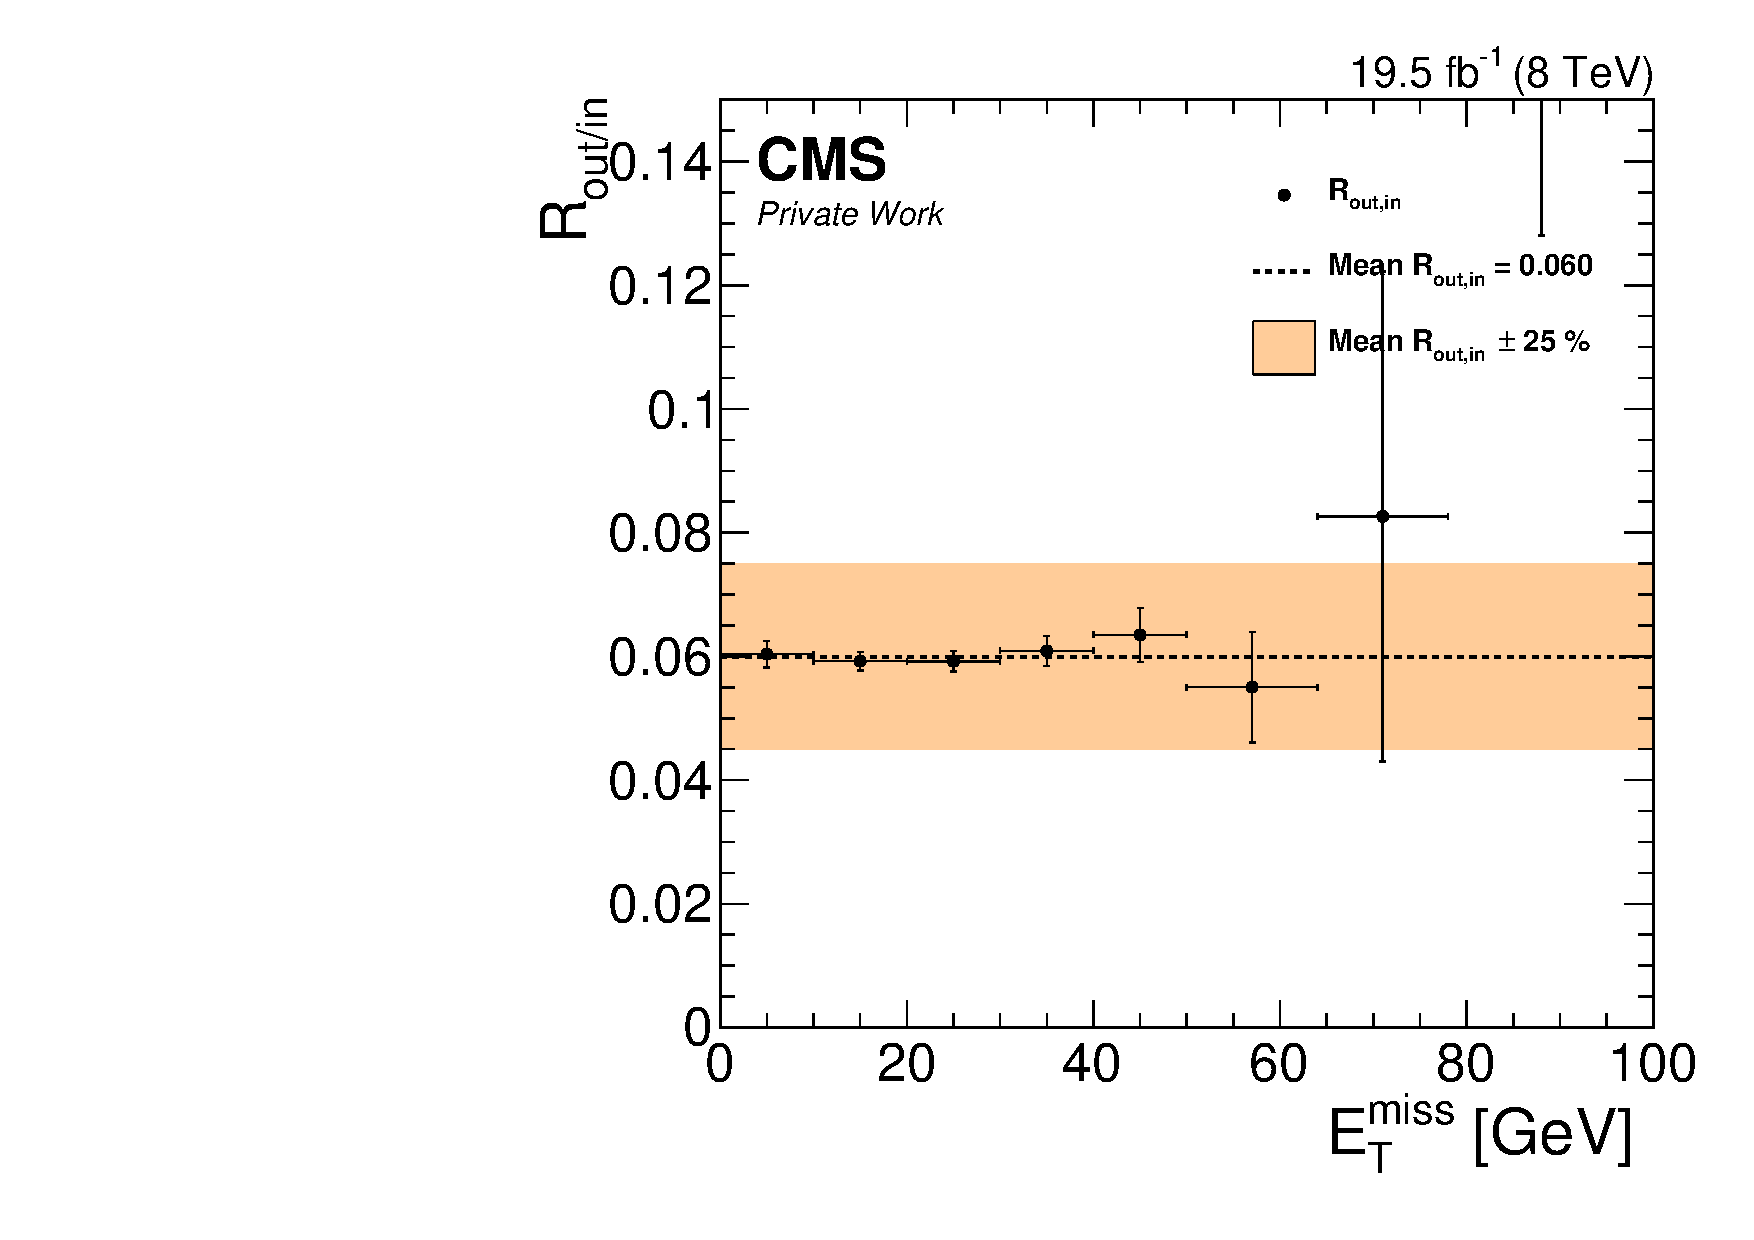
\includegraphics[width=\textwidth]{plots/BG/rOutIn/rOutInSyst_DrellYanControlForward_Full2012_MET_LowMass_SF_None.pdf}
\end{minipage}
\begin{minipage}[t]{0.49\textwidth}
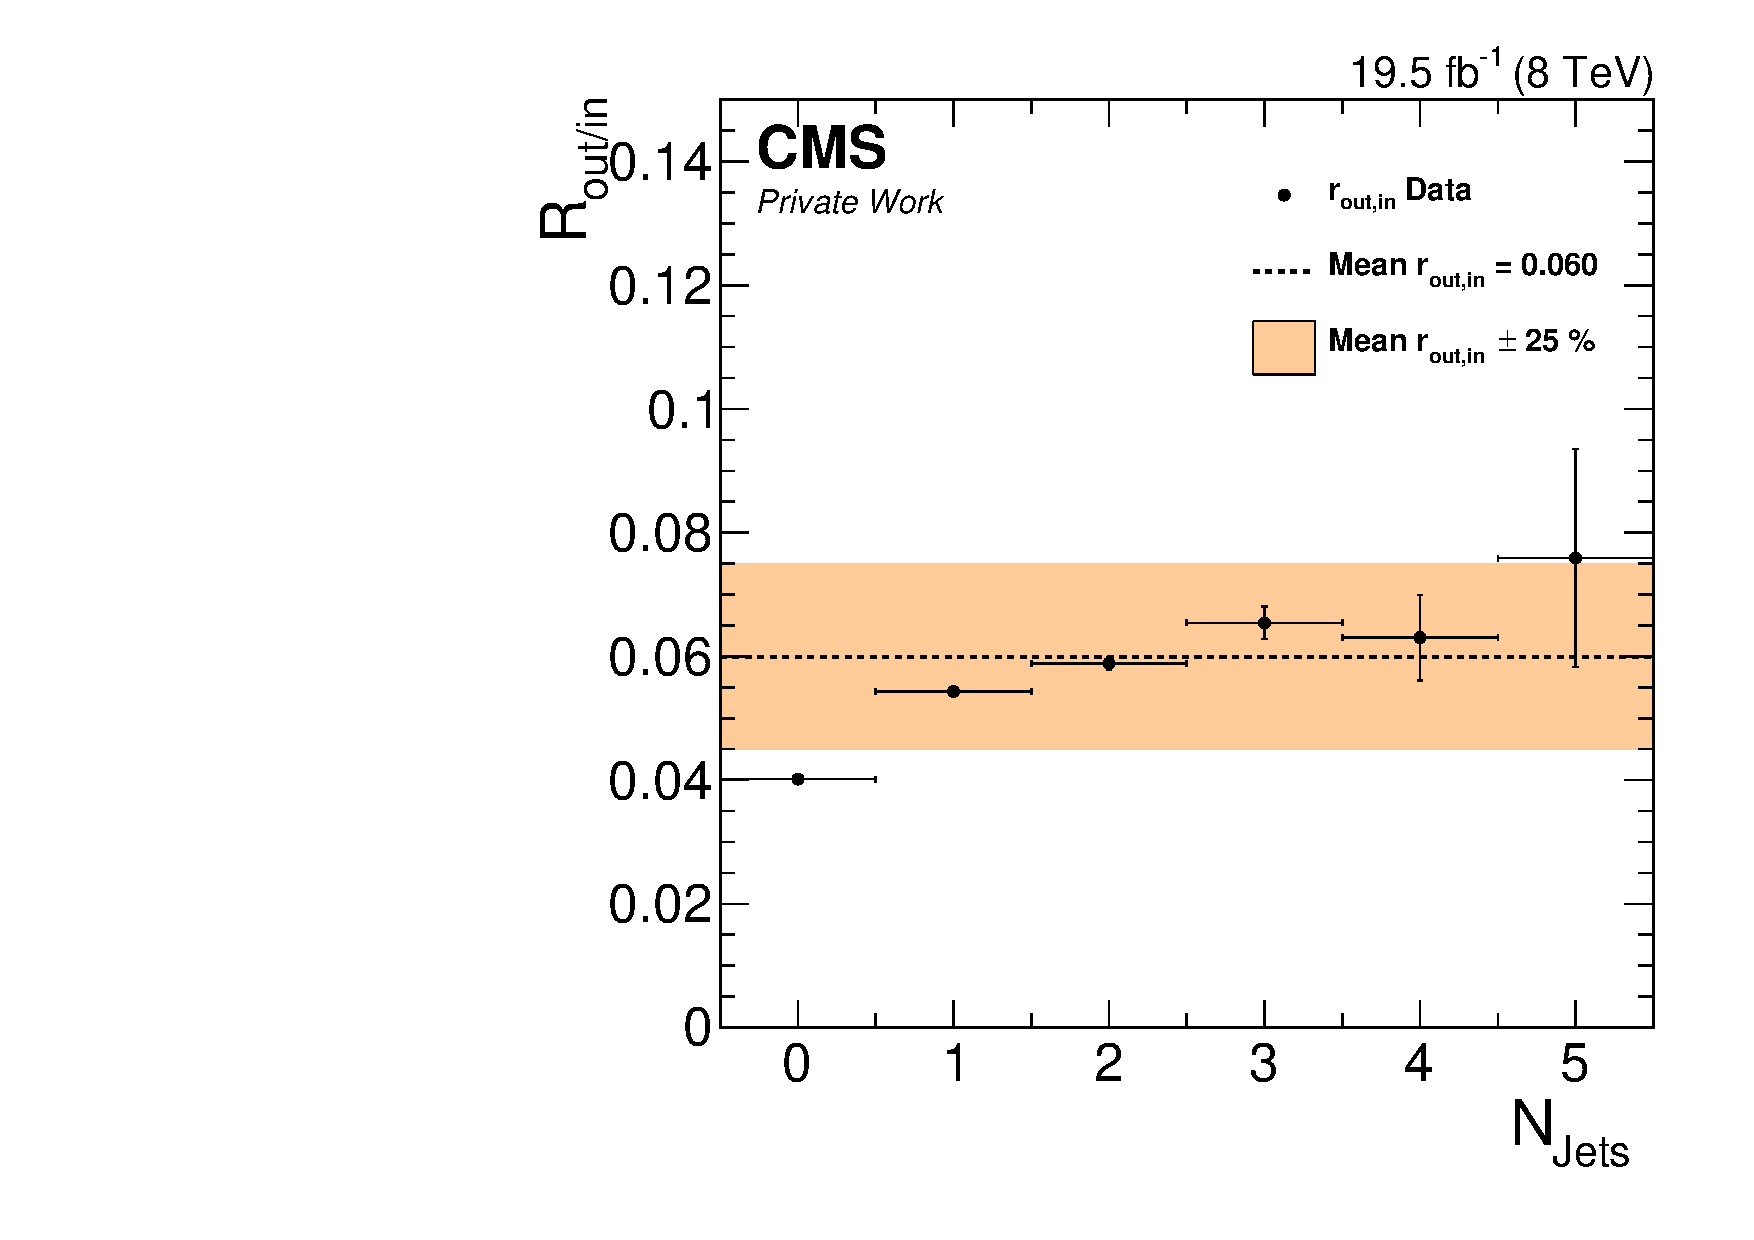
\includegraphics[width=\textwidth]{plots/BG/rOutIn/rOutInSyst_DrellYanControlForward_Full2012_NJets_LowMass_SF_None.pdf}
\end{minipage}
\caption{Dependencies of \Routin on \MET (left) and $N_{jets}$ (right) for the central (top) and forward (bottom) lepton selection. The results on data are shown in black. The central value is shown as a black dashed line while the systematic uncertainty is shown as an orange band.}
\label{fig:ROutInDependencies}
\end{figure} 


\subsection{Resulting background prediction}
The predictions for the on-\Z region from the \JZB and \MET templates methods agree within their uncertainties. As for the \Rsfof factor, a weighted average is used to combine the two estimates. The results of both methods as well as the combination are shown in Table~\ref{tab:dyResults}. Shown there are also the \Routin values and the resulting estimates for the low- and high-Mass regions. For this, the on-Z predictions, which are derived on the PromptReco, are scaled by 1.03$\pm$0.03 to take into account the slight increase in jet multiplicity in the ReReco dataset. 

\begin{table}[!htbp]
 \renewcommand{\arraystretch}{1.2}
 \begin{center}
  \caption{Estimate of the \Z background yields in the \Z peak region and extrapolation to the signal mass region for the full dataset.}
  \begin{tabular}{l|cc|c|}
   \hline
   \hline
                                    & \multicolumn{3}{c|}{\central}            \\
                                    & \EE                   & \MM                   & SF          \\
   \hline
   \Z bkgd estimate (\JZB)                  & $57.9\pm13.8\pm10.1$   & $46.1\pm13.8\pm8.0$          &    $104\pm21\pm18$  \\
   
   \Z bkgd estimate (\MET templates) & $63.2\pm 4.3\pm 15.3$    & $69.5\pm 4.0\pm 16.9$       &    $133\pm7\pm32$  \\
   \Z bkgd estimate (Combined)         & $60.7\pm 11.6$                & $56.8\pm 11.7$                   &    $116\pm21$  \\
   \hline
       \Routin low-Mass       &  0.069$\pm$0.001$\pm$0.017                   & 0.075$\pm$0.001$\pm$0.019            &  0.072$\pm$0.001$\pm$0.018    \\
 
   \hline
     low-Mass estimate    & 4.3$\pm$1.3        & 4.4$\pm$1.4  &  8.6$\pm$2.7 \\

   \hline
       \Routin high-Mass       &  0.025$\pm$0.001$\pm$0.006                   & 0.020$\pm$0.001$\pm$0.005            &  0.022$\pm$0.001$\pm$0.006    \\
 
   \hline
     high-Mass estimate    & 1.5$\pm$0.5        & 1.2$\pm$0.4  &  2.7$\pm$0.8 \\
  
   \hline
                                    & \multicolumn{3}{c|}{\forward} \\
                                    & \EE                  & \MM                        & SF \\
   \hline
   \Z bkgd estimate (\JZB)                   & $15.6\pm 8.3\pm 2.9$ & $13.8 \pm 8.3\pm 2.8$       & $29\pm11\pm6$ \\
   \Z bkgd estimate (MET templates)          & $24.4\pm 1.8\pm 6.0$ & $32.3\pm 2.2\pm 7.9$       & $56.9\pm3.6\pm14.0$ \\
   \Z bkgd estimate (Combined)          & $21\pm 5$        & $25\pm 6$             & $42\pm 9$  \\

   \hline
       \Routin low-Mass       &  0.055$\pm$0.001$\pm$0.014                   & 0.064$\pm$0.001$\pm$0.016            &  0.060$\pm$0.001$\pm$0.015    \\

   \hline
     low-Mass estimate    & 1.2$\pm$0.4        & 1.6$\pm$0.6  &  2.6$\pm$0.8 \\


   \hline
       \Routin high-Mass       &  0.031$\pm$0.001$\pm$0.008                   & 0.026$\pm$0.001$\pm$0.007            &  0.028$\pm$0.001$\pm$0.007    \\

   \hline
     high-Mass estimate    & 0.7$\pm$0.2        & 0.7$\pm$0.2  &  1.2$\pm$0.4 \\

   \hline
   \hline
 \end{tabular}
 \label{tab:dyResults}
 \end{center}
\end{table}






\section{Search for a kinematic edge with a fit}
